\documentclass[11pt]{article}
\usepackage[utf8]{inputenc}
\usepackage[spanish]{babel}
\decimalpoint
\usepackage{amsmath}
\usepackage{amsthm}
\usepackage{amssymb}
\usepackage{graphicx}
\usepackage[margin=0.8in]{geometry}
\usepackage{fancyhdr}
\usepackage[inline]{enumitem}
\usepackage{float}
\usepackage{cancel}
\usepackage{bigints}
\usepackage{listings}
\usepackage{xcolor}
\usepackage{listingsutf8}
\usepackage{algpseudocode}
\usepackage{algorithm}
\usepackage{apacite}
\usepackage{tcolorbox}
\usepackage{multicol}
\usepackage{tipa}
\usepackage{caption} 
\pagestyle{fancy}
\usepackage{hyperref}
\usepackage{mathtools}% http://ctan.org/pkg/mathtools
\renewcommand{\labelenumii}{\theenumii}
\renewcommand{\theenumii}{\theenumi.\arabic{enumii}.}
\hypersetup{
    colorlinks,
    citecolor=black,
    filecolor=black,
    linkcolor=black,
    urlcolor=black
}
\newcommand{\xvdash}[1]{%
	\vdash^{\mkern-10mu\scriptscriptstyle\rule[-.9ex]{0pt}{0pt}#1}%
}
\setlength{\headheight}{15pt} 
\lhead{Tarea 10. Replicación de un sistema completo en la nube}
\rhead{\thepage}
\lfoot{ESCOM-IPN}
\renewcommand{\footrulewidth}{0.5pt}
\setlength{\parskip}{0.5em}
\newcommand{\ve}[1]{\overrightarrow{#1}}
\newcommand{\abs}[1]{\left\lvert #1 \right\lvert}
\newcommand{\blank}{\text{\textcrb}}
\date{\today}
\title{Tarea 10. Replicación de un sistema completo en la nube}
\author{Sanchez Mendez Edmundo Josue}

\lstset{
tabsize = 4, %% set tab space width
showstringspaces = false, %% prevent space marking in strings, string is defined as the text that is generally printed directly to the console
numbers = left, %% display line numbers on the left
commentstyle = \color{green}, %% set comment color
keywordstyle = \color{blue}, %% set keyword color
stringstyle = \color{red}, %% set string color
rulecolor = \color{black}, %% set frame color to avoid being affected by text color
basicstyle = \small \ttfamily , %% set listing font and size
breaklines = true, %% enable line breaking
numberstyle = \tiny,
}

\bibliographystyle{apacite}
\begin{document}
		\begin{titlepage}
			\begin{center}
				
				% Upper part of the page. The '~' is needed because \\
				% only works if a paragraph has started.
				
				\noindent
				\begin{minipage}{0.5\textwidth}
					\begin{flushleft} \large
						
\includegraphics[width=0.5\textwidth]{resources/ipn.png}
					\end{flushleft}
				\end{minipage}%
				\begin{minipage}{0.55\textwidth}
					\begin{flushright} \large
						
\includegraphics[width=0.5\textwidth]{resources/escom.png}
					\end{flushright}
				\end{minipage}
				
				\textsc{\LARGE Instituto Politécnico Nacional}\\[0.5cm]
				
				\textsc{\Large Escuela Superior de Cómputo}\\[1cm]
				
				% Title
				
				{ \huge Tarea 10. Replicación de un sistema completo en la nube \\[1cm] }
				
				{ \Large Unidad de aprendizaje: Desarrollo de Sistemas Distribuidos} \\[1cm]
				
				{ \Large Grupo: 4CV11 } \\[1cm]
				
				\noindent
				\begin{minipage}{0.5\textwidth}
					\begin{flushleft} \large
						\emph{Alumno:} \\
						Sanchez Mendez Edmundo Josue
					\end{flushleft}
				\end{minipage}%
				\begin{minipage}{0.5\textwidth}
					\begin{flushright} \large
						\emph{Profesor:} \\
						Pineda Guerrero Carlos 
					\end{flushright}
				\end{minipage}
				
				\vfill
				% Bottom of the page
				{\large {\today}}
			\end{center}
		\end{titlepage}
	
	\titlepage
	\tableofcontents
	\newpage
	
	\section{Introducción}
	La tarea consiste en replicar una plataforma de servicios web basada en Tomcat y MySQL, utilizando el programa SimpleProxyServer.java como administrador de tráfico.

	Se deberá crear dos máquina virtuales en la nube de Azure con Ubuntu 18 a partir de la imagen creada en la tarea 6.

	El cliente se conectará al programa SimpleProxyServer.java el cual a su vez se conectará al servidor Tomcat en la máquina virtual 1 (sistema principal).

	El proxy también se conectará al servidor Tomcat que ejecuta en la máquina virtual 2 (réplica).

	El servidor Tomcat que ejecuta en la máquina virtual 1 enviará una respuesta al programa SimpleProxyServer.java y este a su vez enviará la respuesta al cliente. 

	El proxy ignorará la respuesta del servidor Tomcat que ejecuta en la maquina virtual 2.
	
	Los pasos a seguir son los siguientes:
		\begin{enumerate}
			\item Crear dos máquinas virtuales en la nube de Azure con Ubuntu 18, 1 GB de RAM y disco HDD estándar a partir de la imagen creada en la tarea 6.
			\item Abrir el puerto 80 protocolo TCP en la máquina virtual 1.
			\item Abrir el puerto 8080 protocolo TCP en la máquina virtual 2, ingresar en el campo ``Origen'' (``Source'' si la pantalla está en inglés) la IP de la máquina virtual 1 (por seguridad, la máquina virtual 1 es la única computadora que podrá acceder la máquina virtual 2).
			\item Conectar a la máquina virtual 1 (sistema principal) utilizando el programa ssh.
			\item Utilizando el programa sftp enviar a la máquina virtual 1 el archivo: SimpleProxyServer.java
			\item Compilar en la máquina virtual 1 el programa SimpleProxyServer.java
			\item Iniciar Tomcat en las máquinas virtuales 1 y 2.
			\item Ejecutar el máquina virtual 1 el proxy:\par
			sudo java SimpleProxyServer ip-maquina-virtual-2 8080 80 8080 \&\par
			Donde IP-máquina-virtual-2 es la IP de la réplica, 8080 es el puerto abierto en la réplica (servidor Tomcat remoto), 80 es el puerto abierto en el sistema principal (proxy local) y 8080 es el puerto en la máquina virtual 1 dónde Tomcat recibe las peticiones (puerto de Tomcat local). Notar que no es necesario abrir el puerto 8080 en la máquina virtual 1, ya que el proxy y Tomcat se comunican localmente mediante loopback.\par
En este caso ejecutamos el proxy con ``sudo'' para que este pueda abrir el puerto 80 en la maquina virtual 1.\par
			\textbf{Probar el servicio web utilizando HTML-Javascript}
			\item En la computadora local (Windows, Linux o MacOS):
				\begin{enumerate}
				    \item Ingresar la siguiente URL en un navegador, notar que no es necesario ingresar el nombre del puerto, ya que se utiliza el puerto default 80:\par http://ip-máquina-virtual-1/prueba.html
 					\item Dar clic en el botón ``Alta usuario'' para dar de alta un nuevo usuario. Capturar los campos y dar clic en el botón ``Alta''.
					\item Mostrar los registros insertados en la base de datos en la maquina virtual principal y la réplica (no desplegar el contenido del campo foto).
					\item Dar clic en el botón ``Consulta usuario'' para consultar el usuario dado de alta en el paso 5.  Capturar el email y dar clic en el botón ``Consulta'',
					\item Modificar algún dato del usuario y dar clic en el botón ``Modifica''.
					\item Mostrar los registros modificados en la base de datos en la maquina virtual principal y la réplica.
					\item Consultar el usuario modificado, para verificar que la modificación se realizó.
					\item Dar clic en el botón ``Borra usuario'' para borrar el usuario.
					\item Mostrar los registros insertados en la base de datos en la maquina virtual principal y la réplica.
					\item Capturar el email del usuario borrado y dar clic en el botón ``Consulta''.
				\end{enumerate}			
		\end{enumerate}
		
	\section{Desarrollo}
		\subsection{Creación de la maquina virtual 0 (Sistema principal)}
En esta parte veremos la creación de la maquina virtual la cual funcionara como nuestro sistema principal para el desarrollo de esta practica.
		\begin{figure}[H]
			\centering
			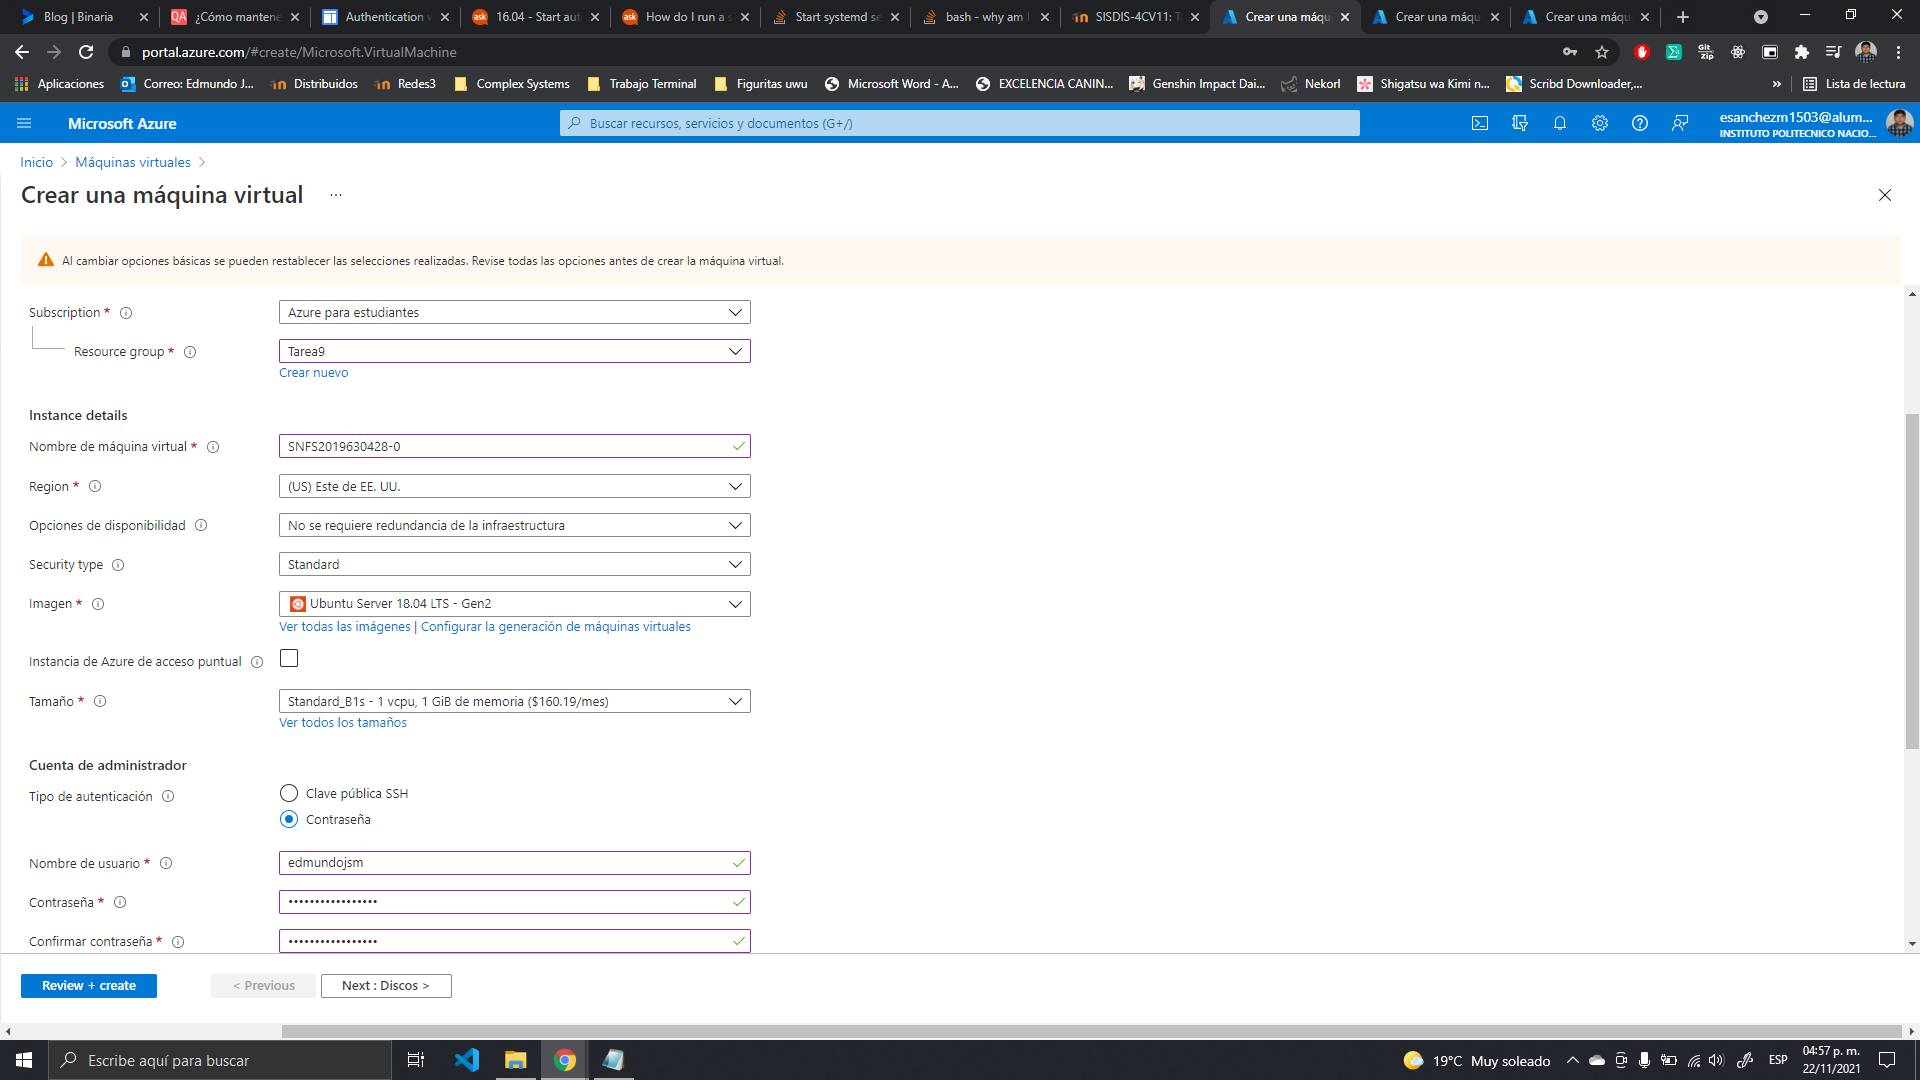
\includegraphics[scale=0.34]{resources/Infobasica0.png}
			\caption{Datos básicos de la maquina virtual.}\label{fig:picture}
		\end{figure}
		\begin{figure}[H]
			\centering
			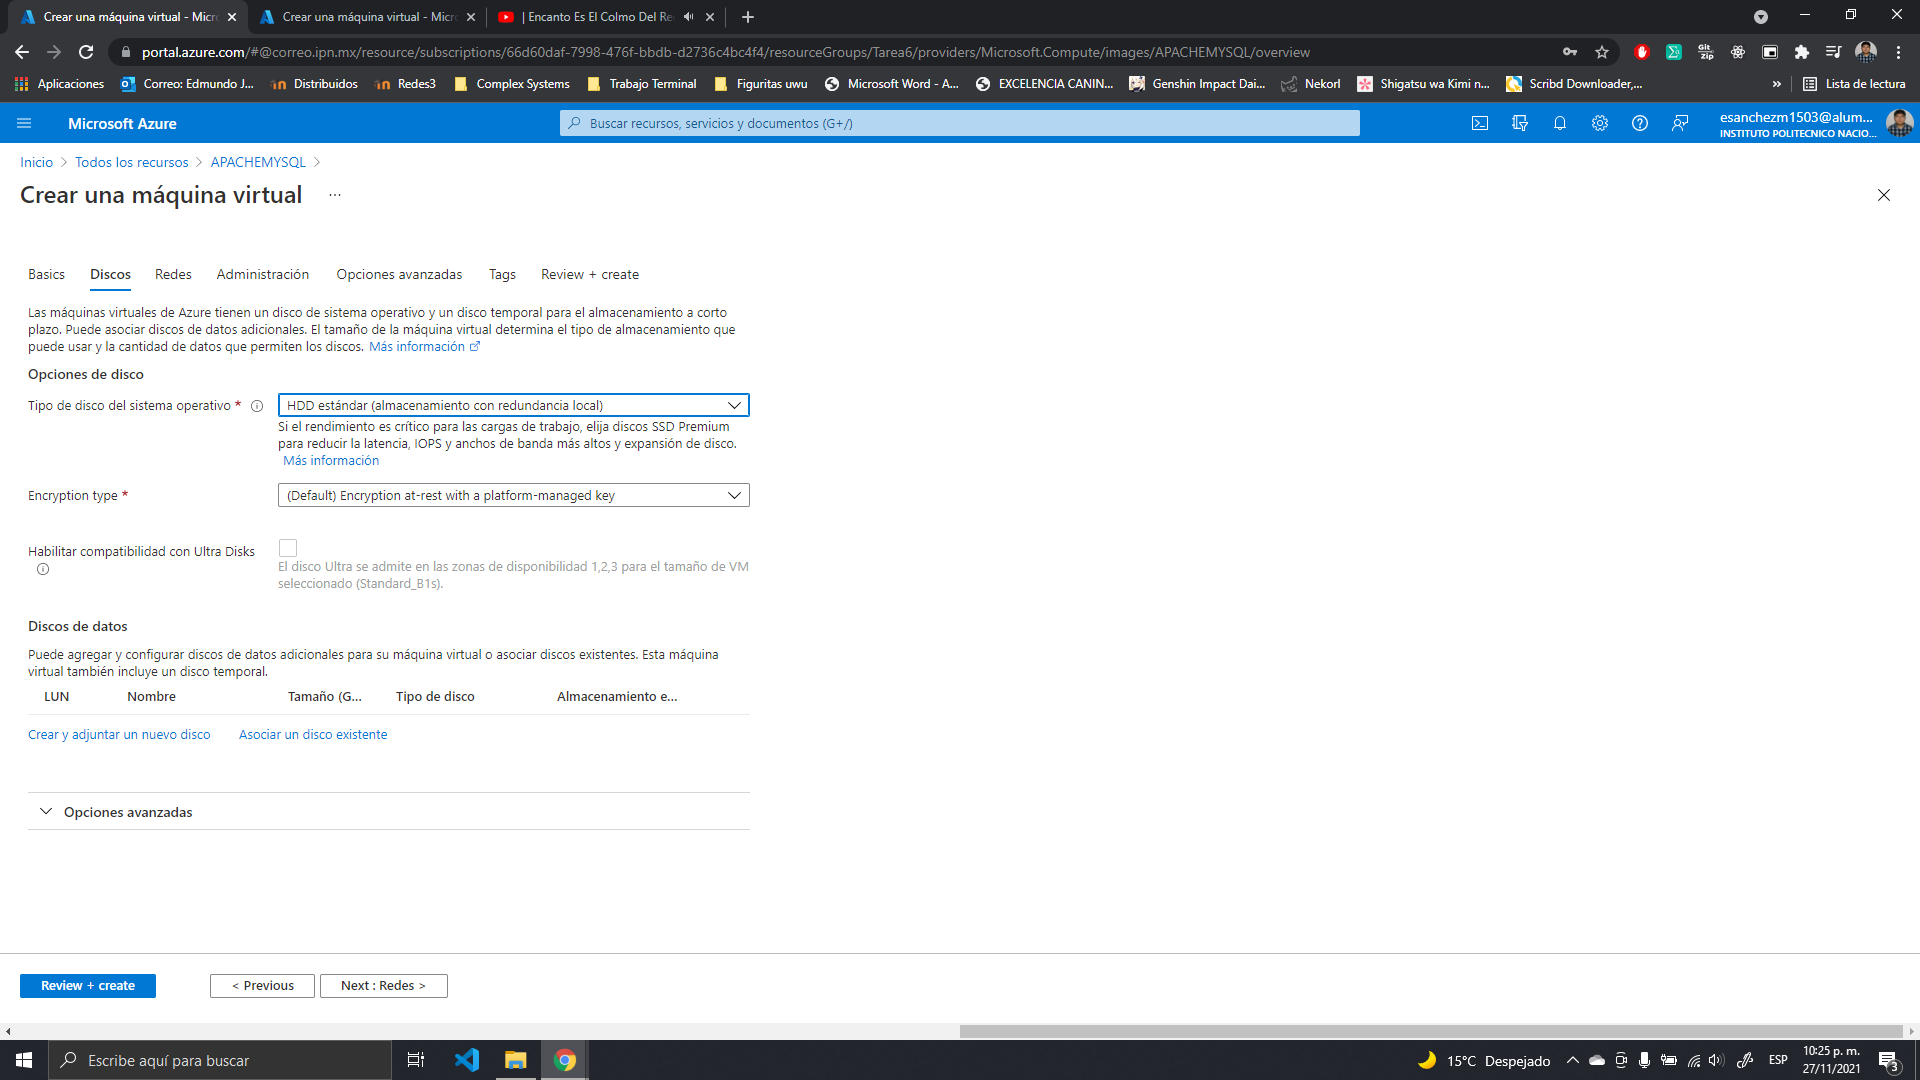
\includegraphics[scale=0.34]{resources/disco0.png}
			\caption{Configuración del tipo de disco de la maquina virtual.}\label{fig:picture}
		\end{figure}
		\begin{figure}[H]
			\centering
			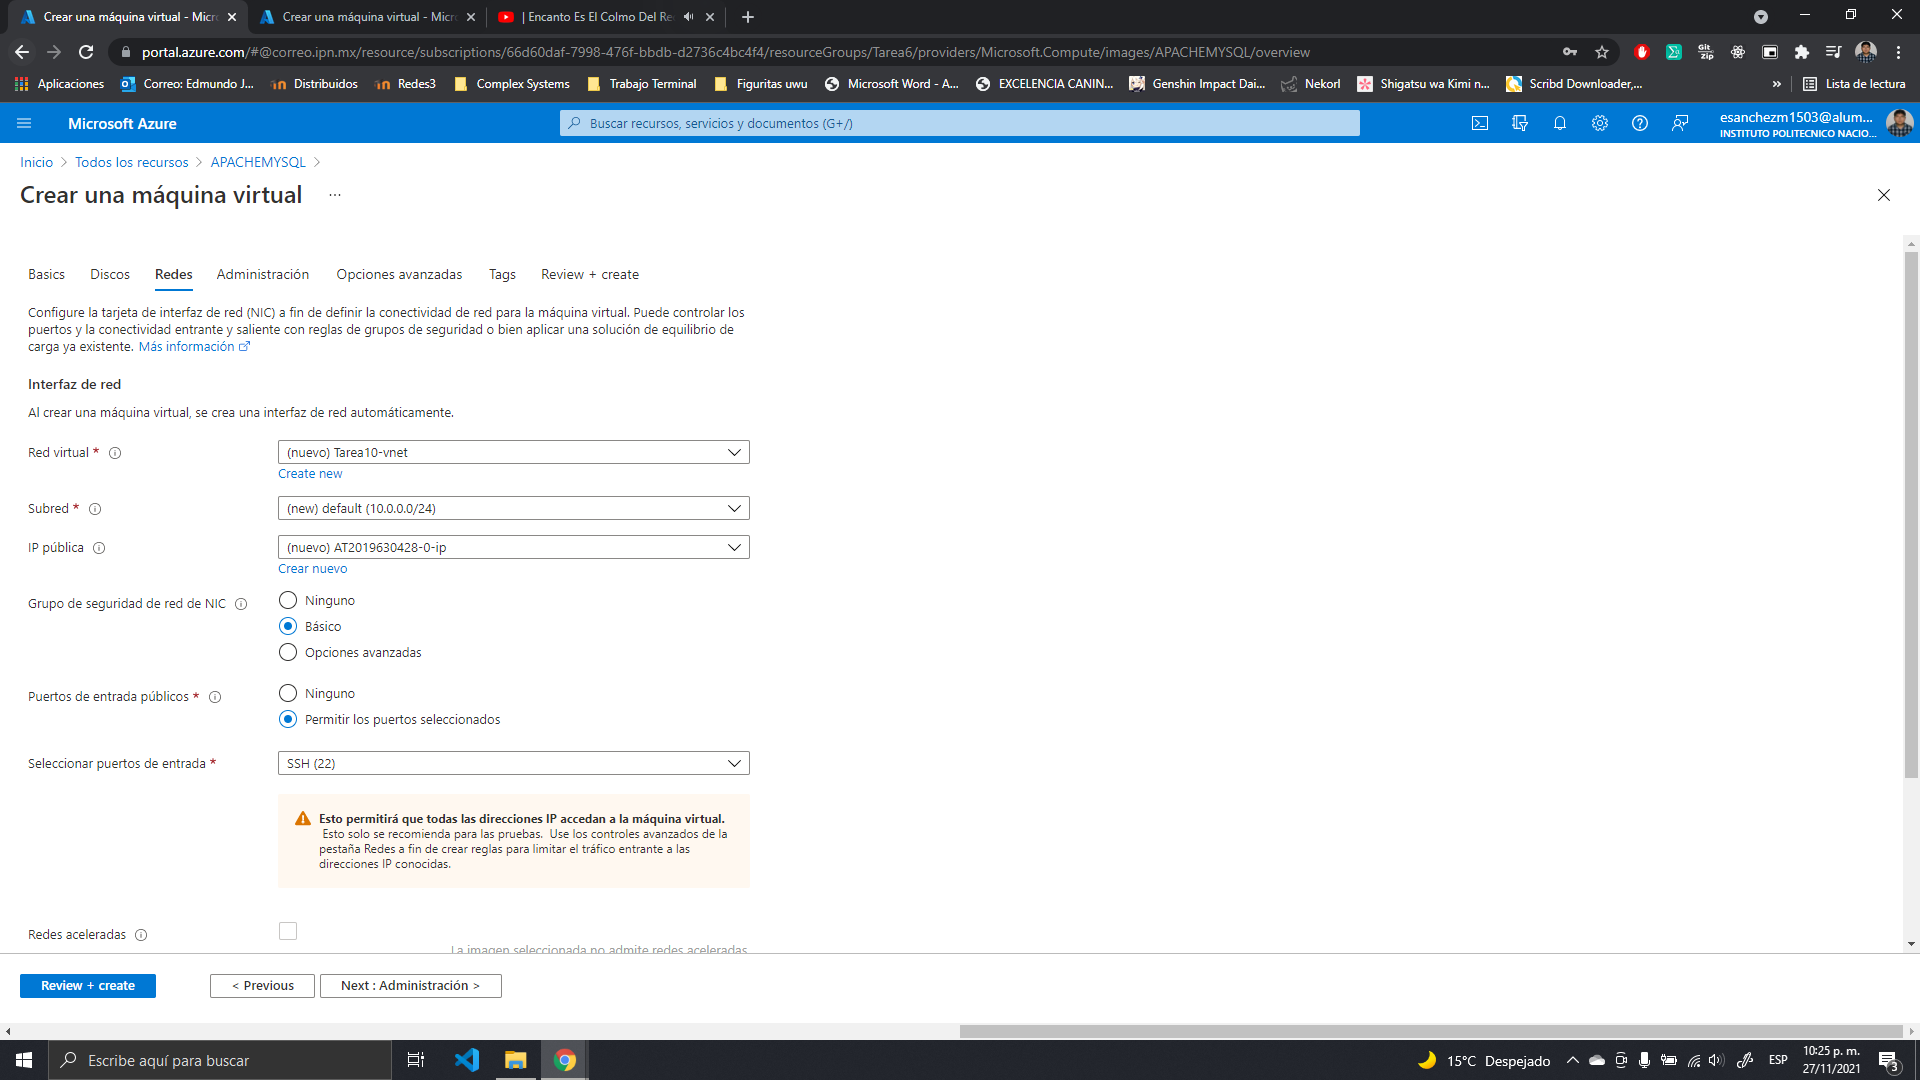
\includegraphics[scale=0.34]{resources/redes0.png}
			\caption{Información sobre la redes de la maquina virtual.}\label{fig:picture}
		\end{figure}
		\begin{figure}[H]
			\centering
			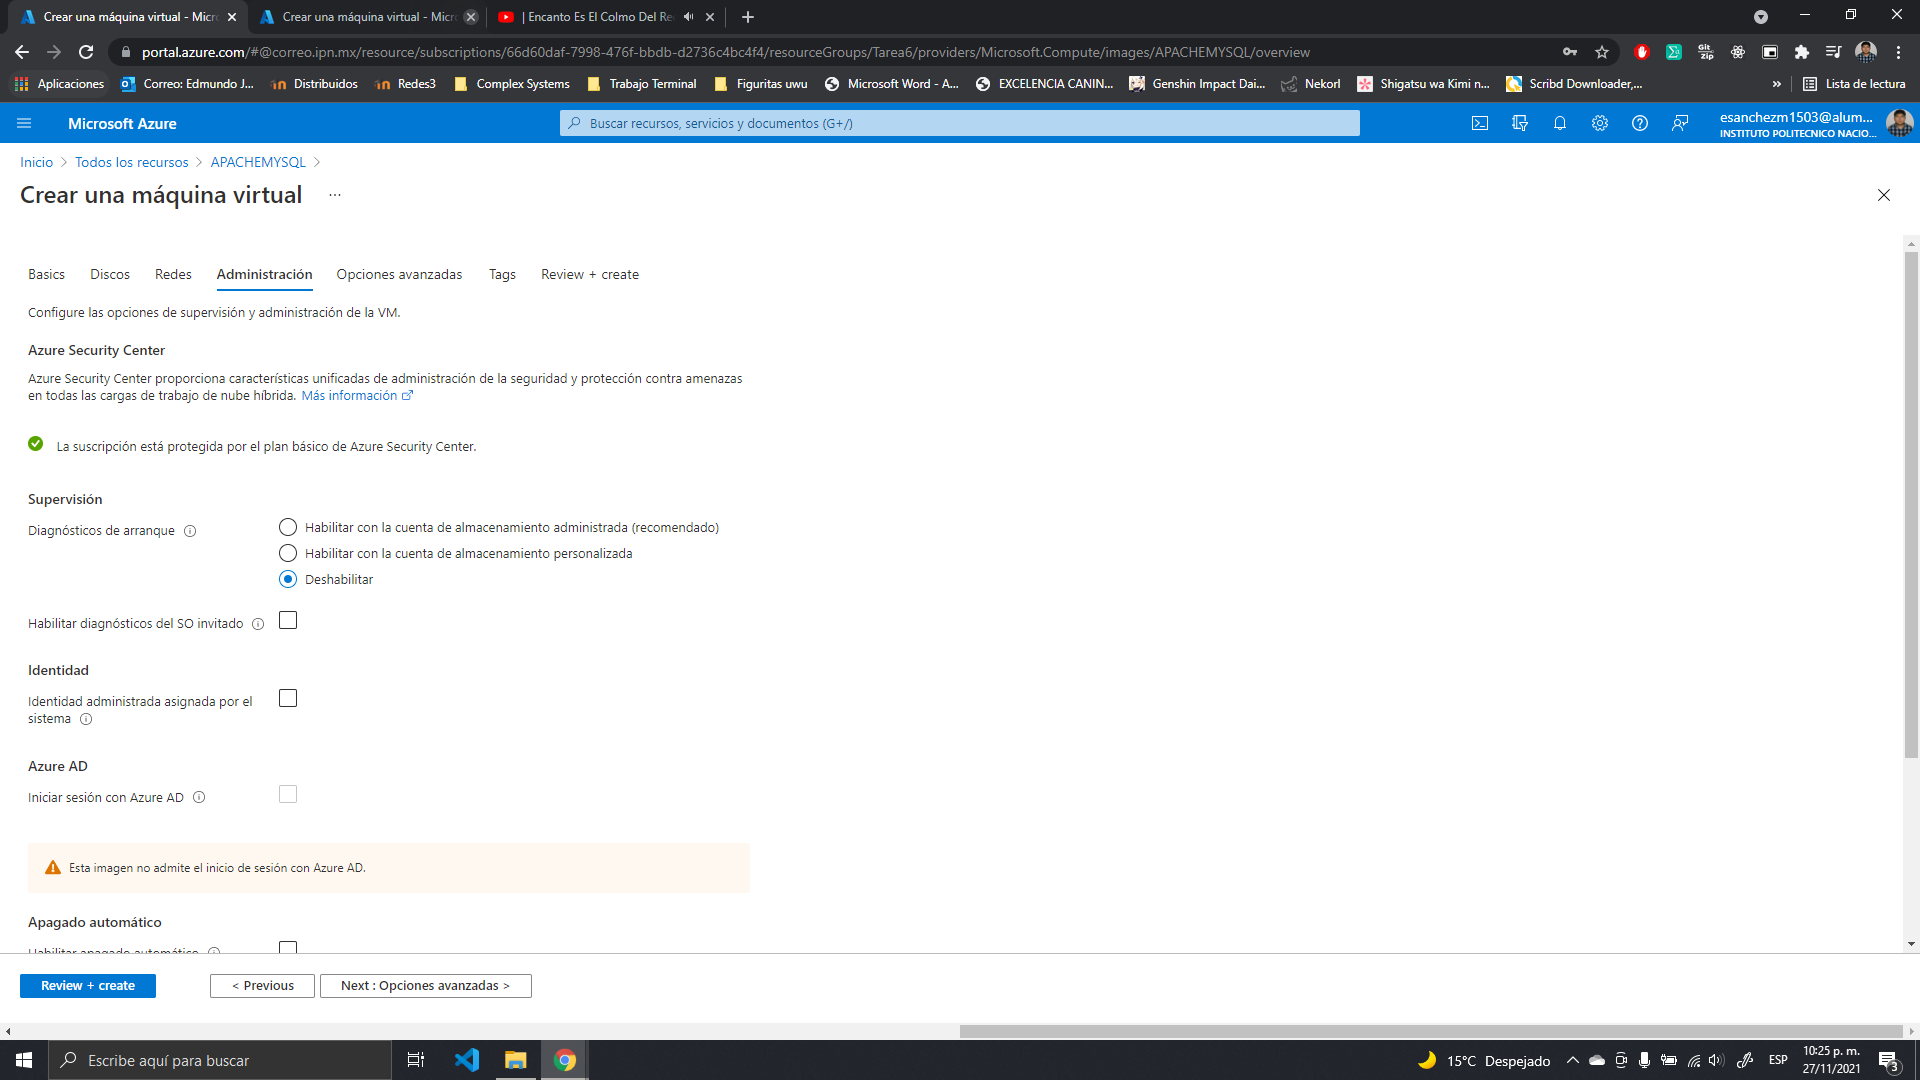
\includegraphics[scale=0.34]{resources/admin0.png}
			\caption{Configuración de la administración de la maquina virtual.}\label{fig:picture}
		\end{figure}
		\begin{figure}[H]
			\centering
			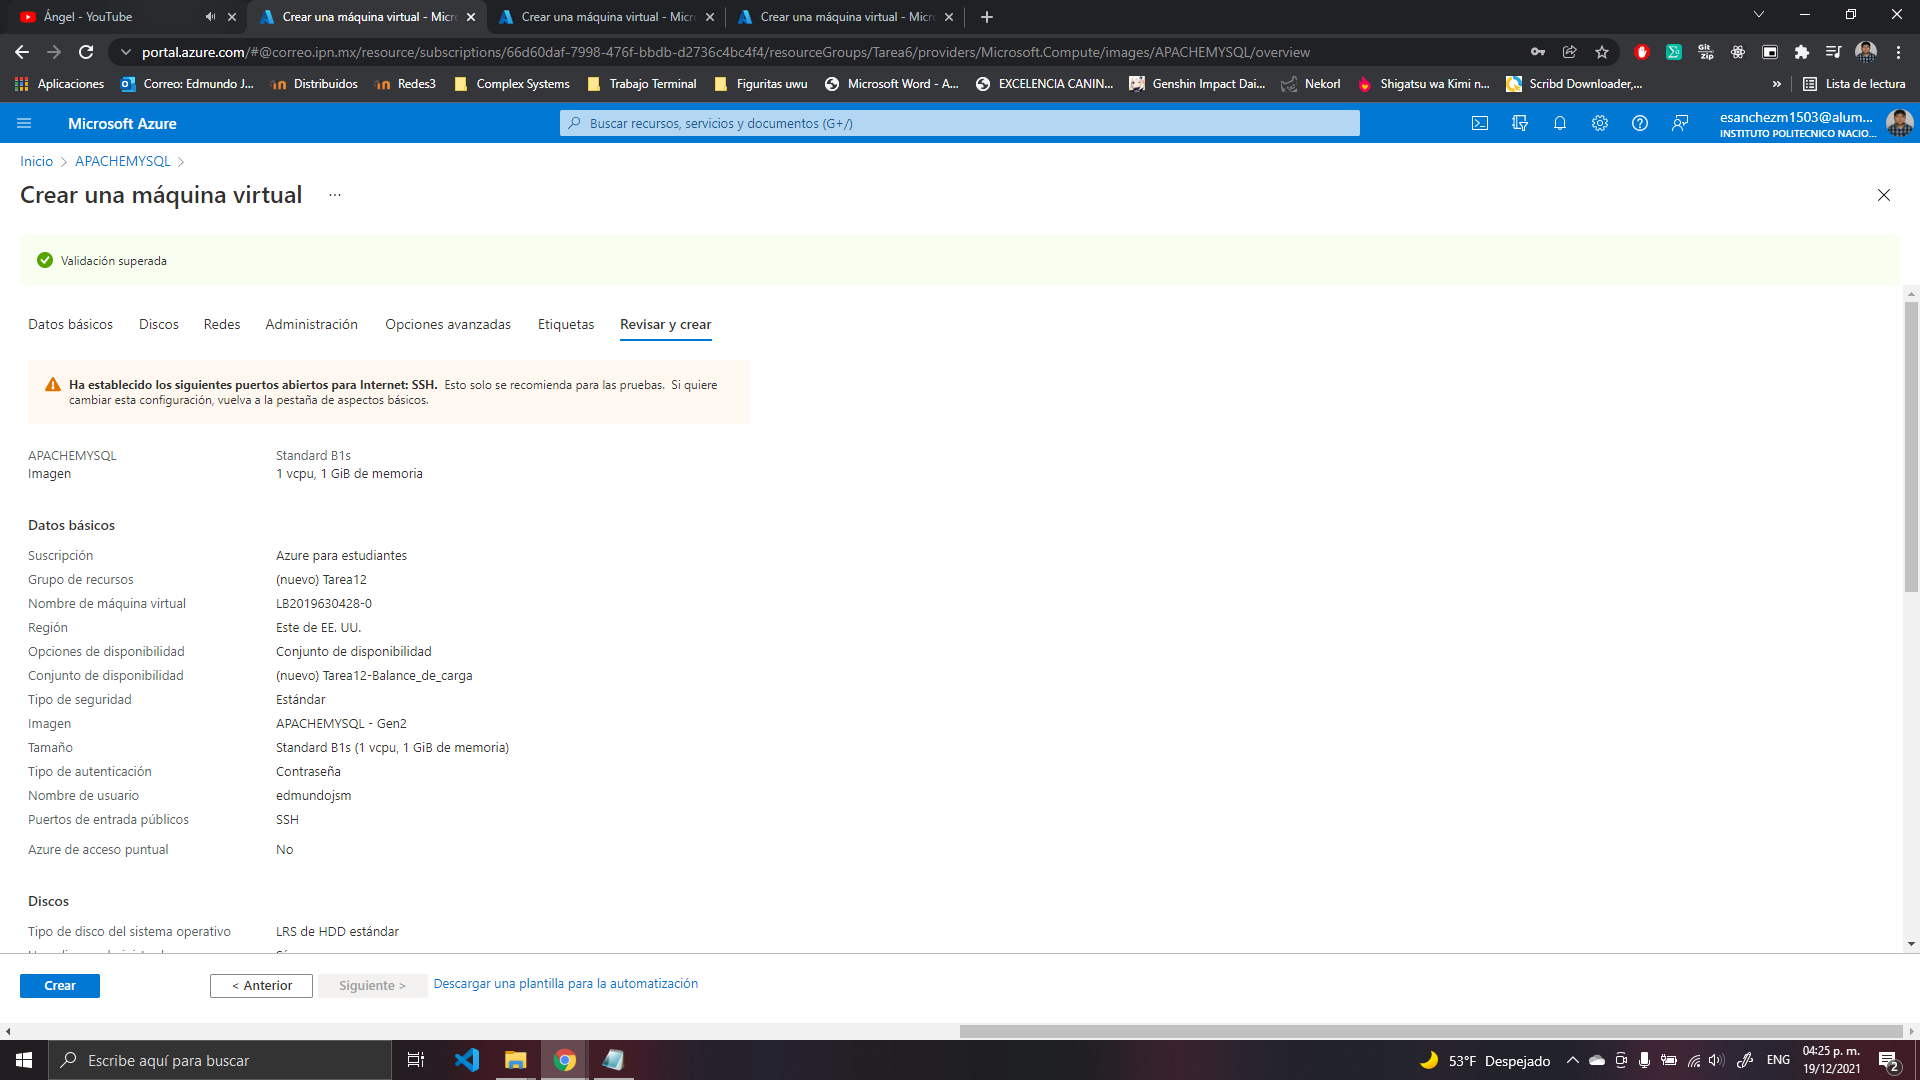
\includegraphics[scale=0.34]{resources/revisarycrear0.png}
			\caption{Creación de la maquina virtual.}\label{fig:picture}
		\end{figure}
		\begin{figure}[H]
			\centering
			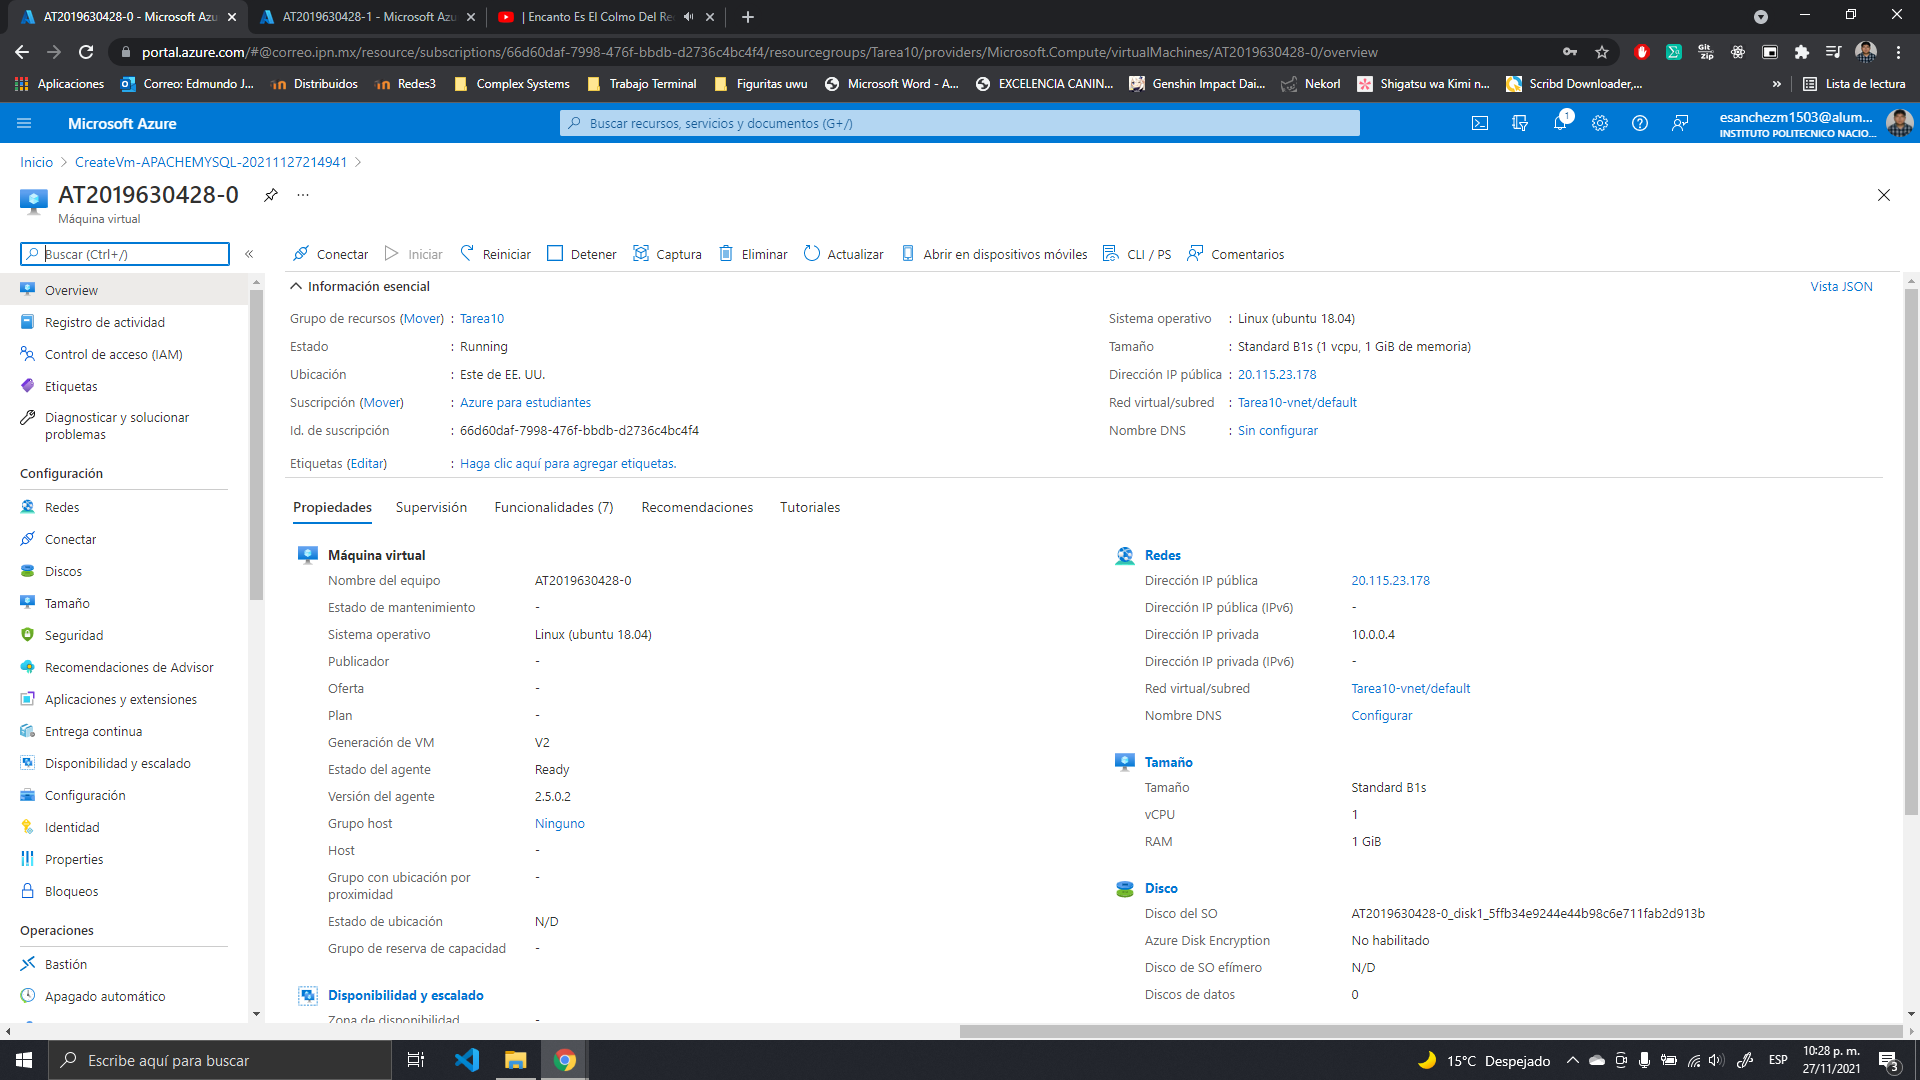
\includegraphics[scale=0.34]{resources/paneldecontrol0.png}
			\caption{Panel de control de la maquina virtual.}\label{fig:picture}
		\end{figure}
		Una vez creada la maquina virtual tenemos que abrir el puerto 80, ya que este puerto es el que ocuparemos como proxy local. En las figuras 7 y 8 podemos ver la configuración del puerto.
		\begin{figure}[H]
			\centering
			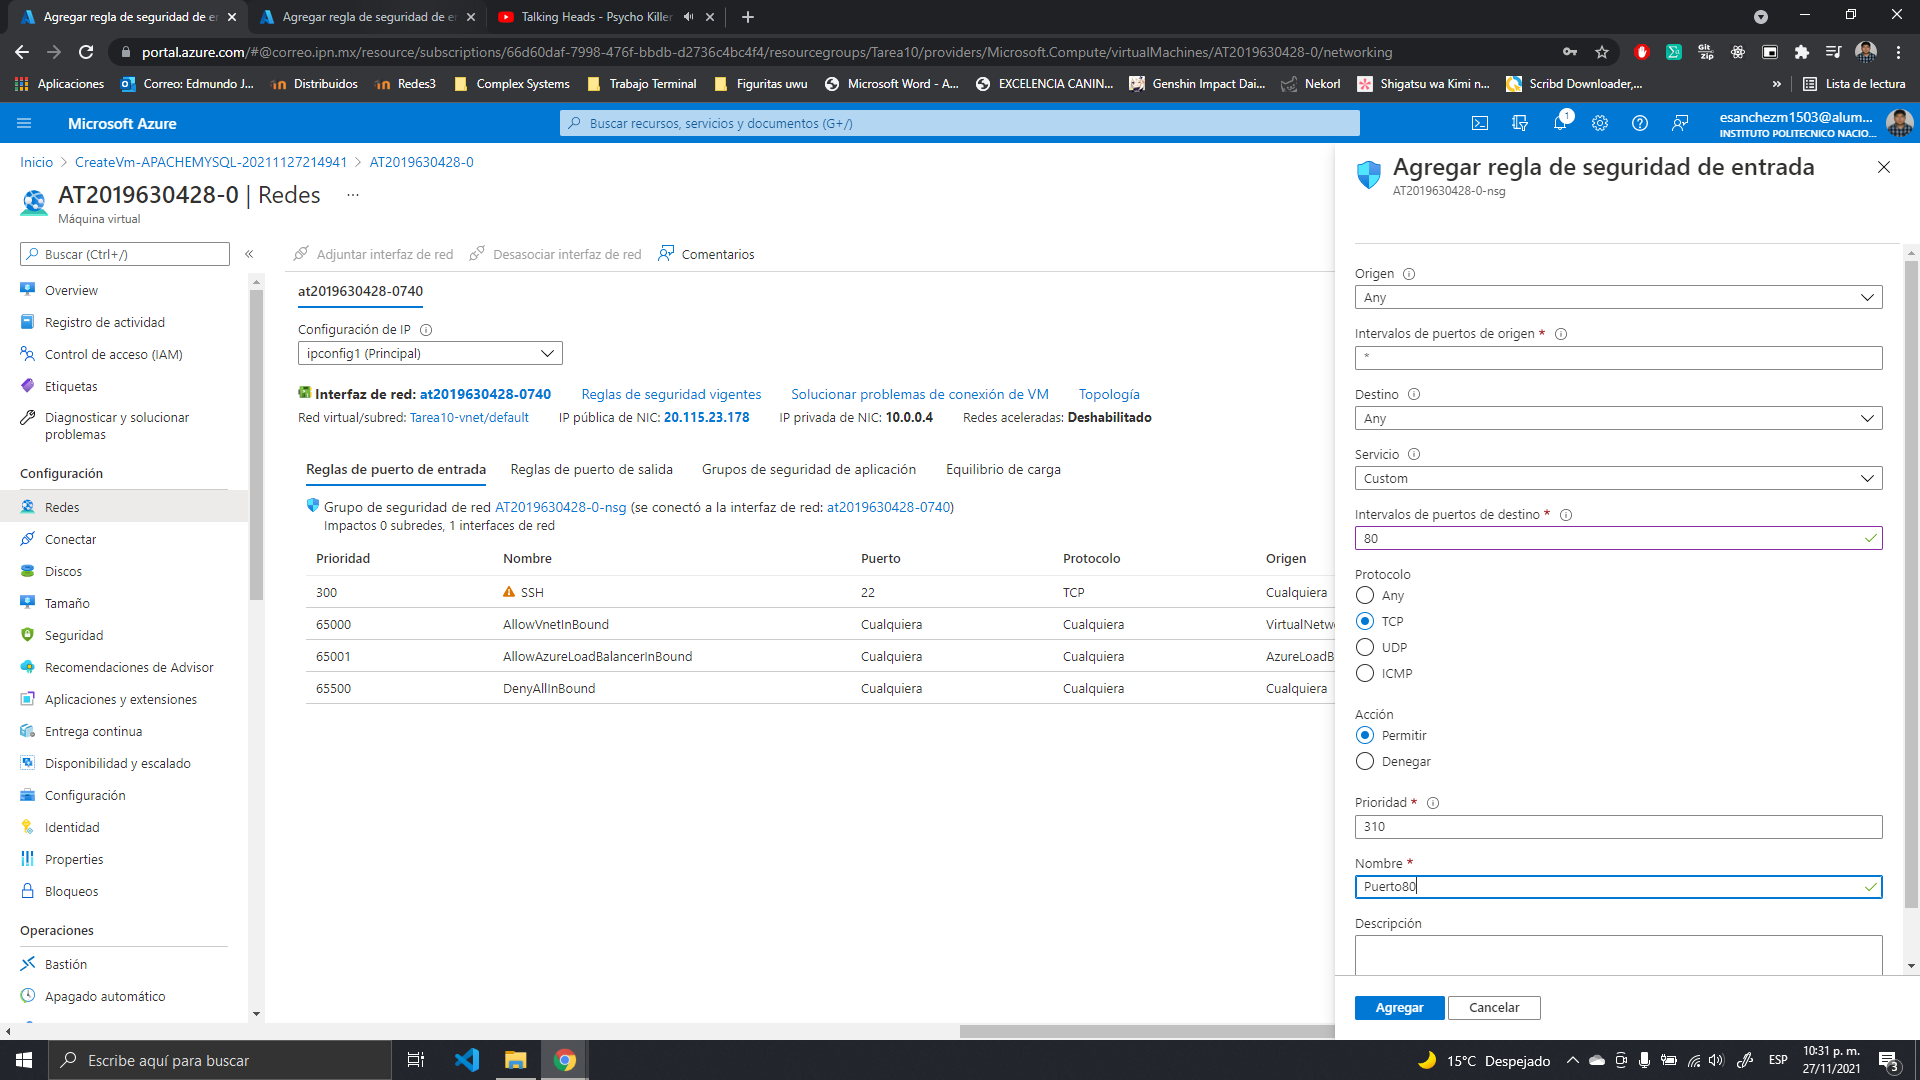
\includegraphics[scale=0.34]{resources/puerto800.png}
			\caption{Configuración del puerto 80.}\label{fig:picture}
		\end{figure}
		\begin{figure}[H]
			\centering
			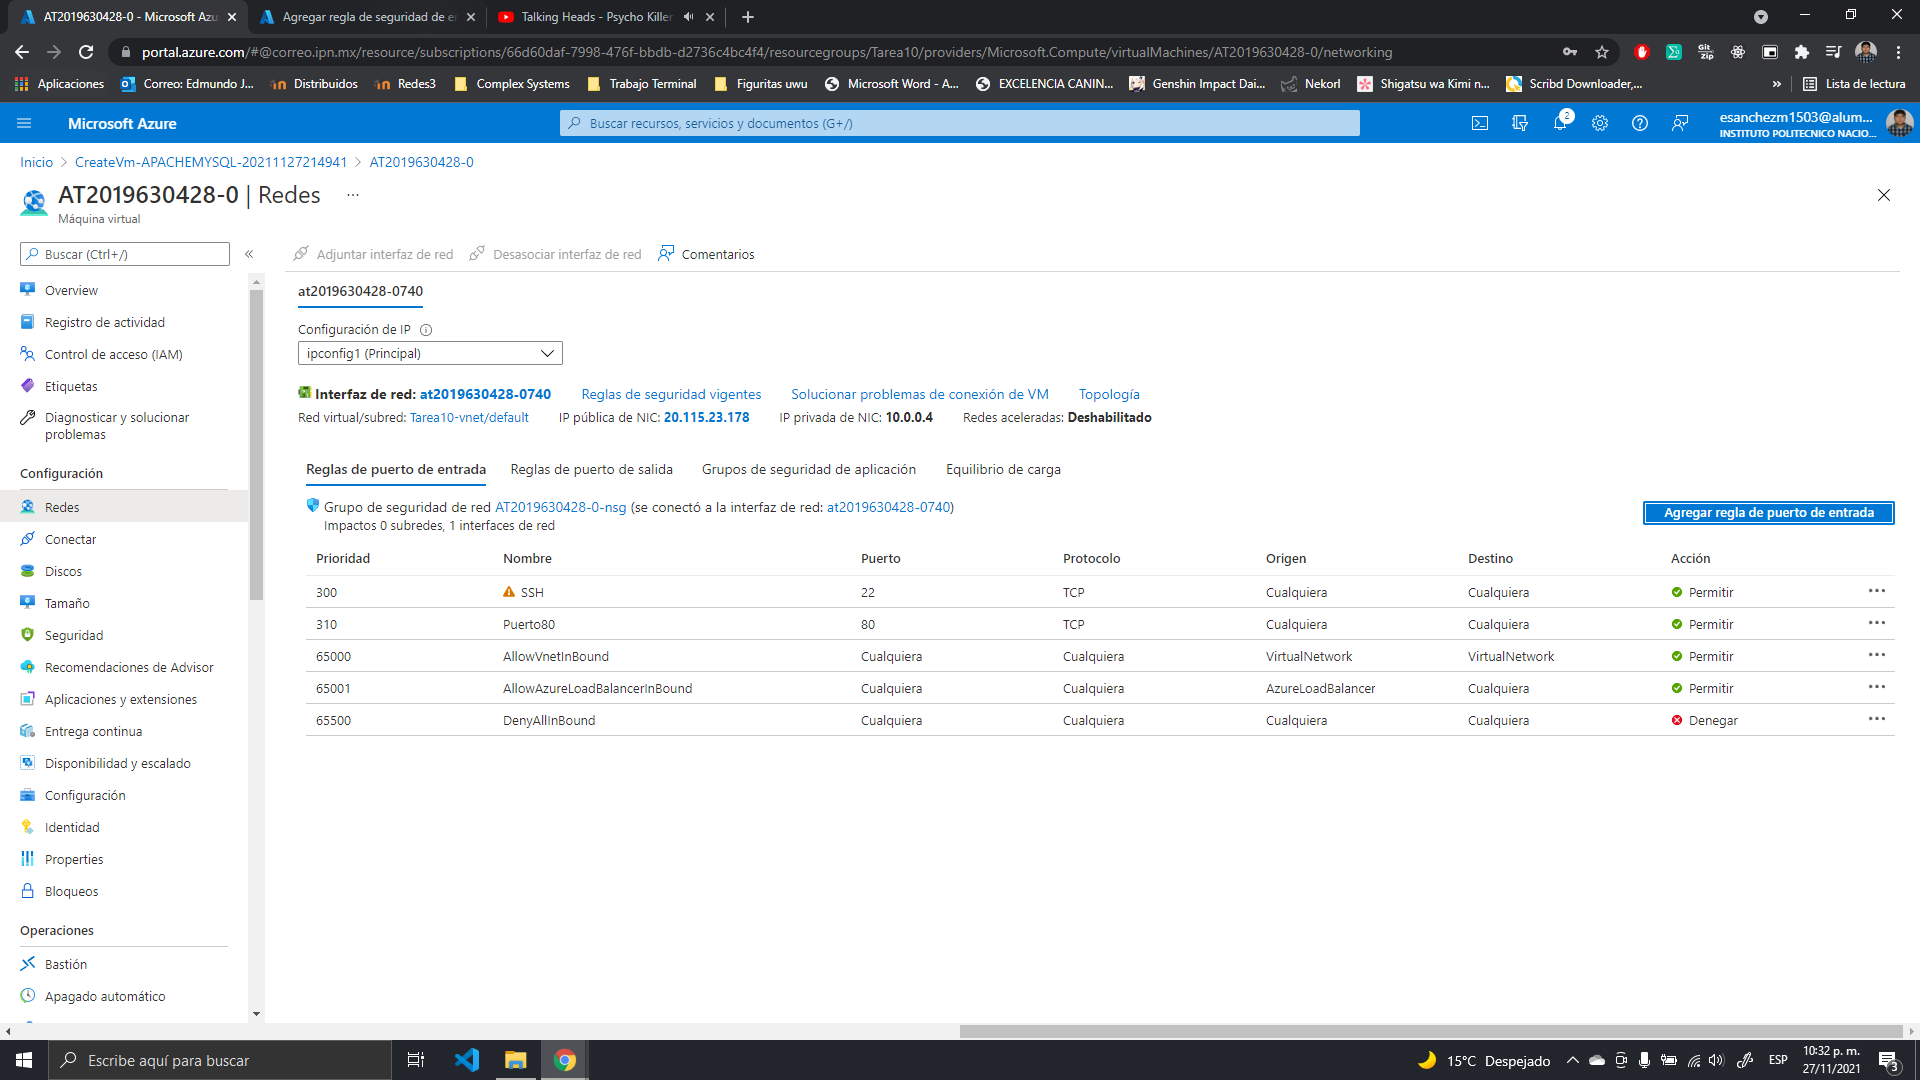
\includegraphics[scale=0.34]{resources/puertook0.png}
			\caption{Puerto 80 abierto correctamente.}\label{fig:picture}
		\end{figure}
		\subsection{Creación de la maquina virtual 1 (Sistema replica)}
En esta parte veremos la creación de la maquina virtual la cual funcionara como nuestro de replica para el desarrollo de esta practica.
		\begin{figure}[H]
			\centering
			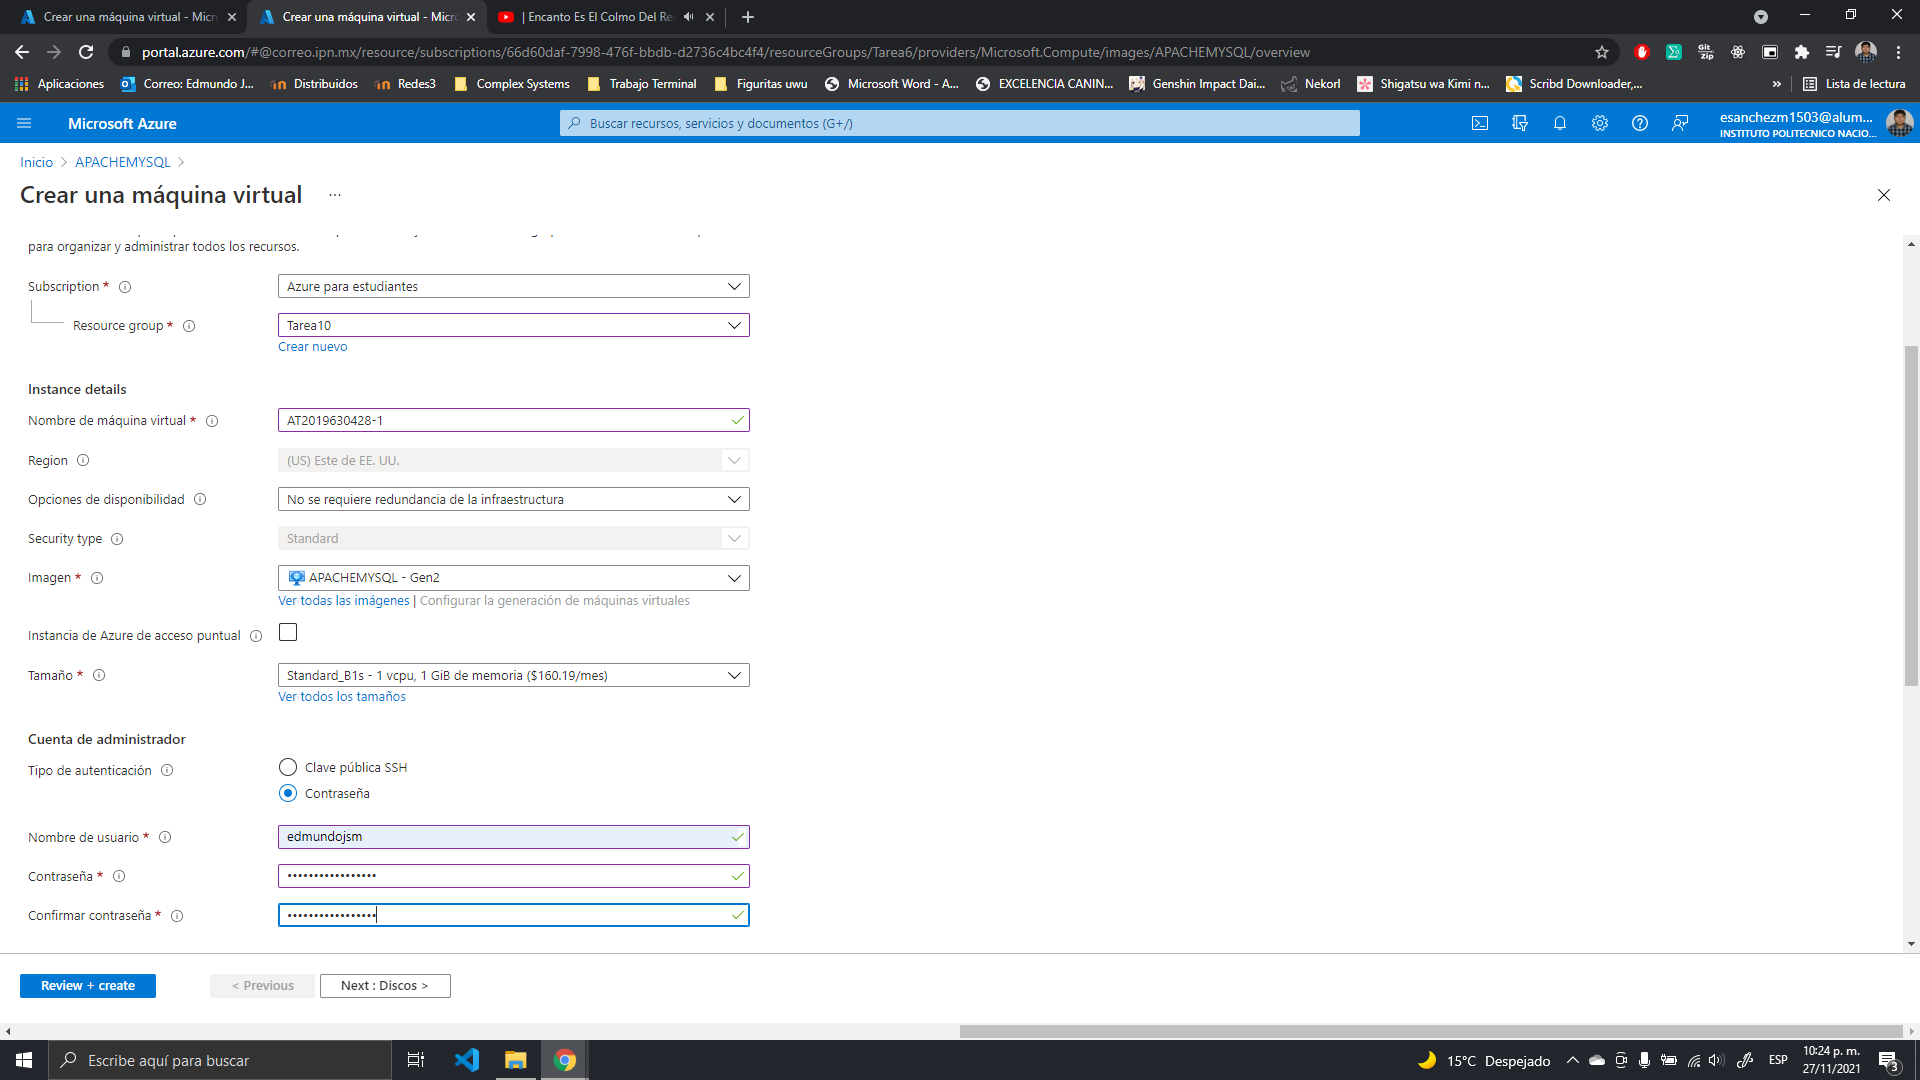
\includegraphics[scale=0.34]{resources/Infobasica1.png}
			\caption{Datos básicos de la maquina virtual.}\label{fig:picture}
		\end{figure}
		\begin{figure}[H]
			\centering
			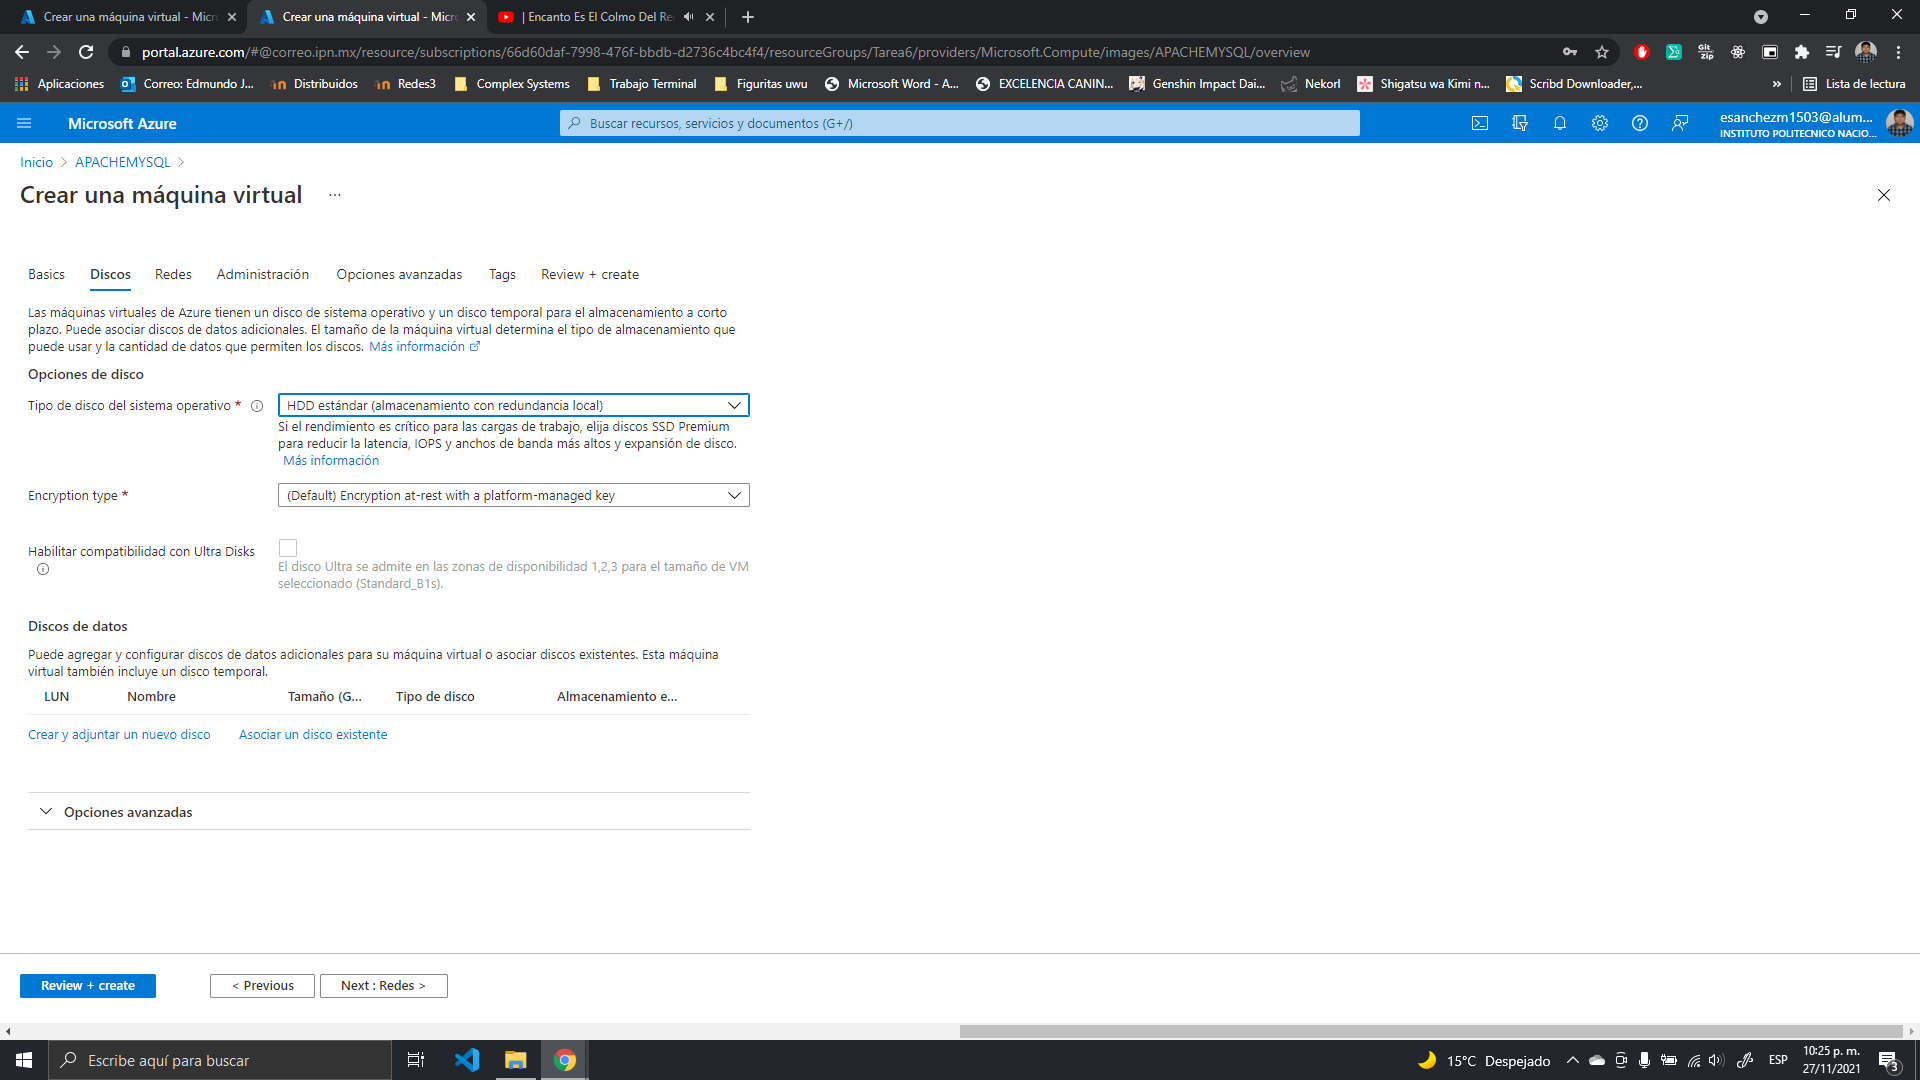
\includegraphics[scale=0.34]{resources/disco1.png}
			\caption{Configuración del tipo de disco de la maquina virtual.}\label{fig:picture}
		\end{figure}
		\begin{figure}[H]
			\centering
			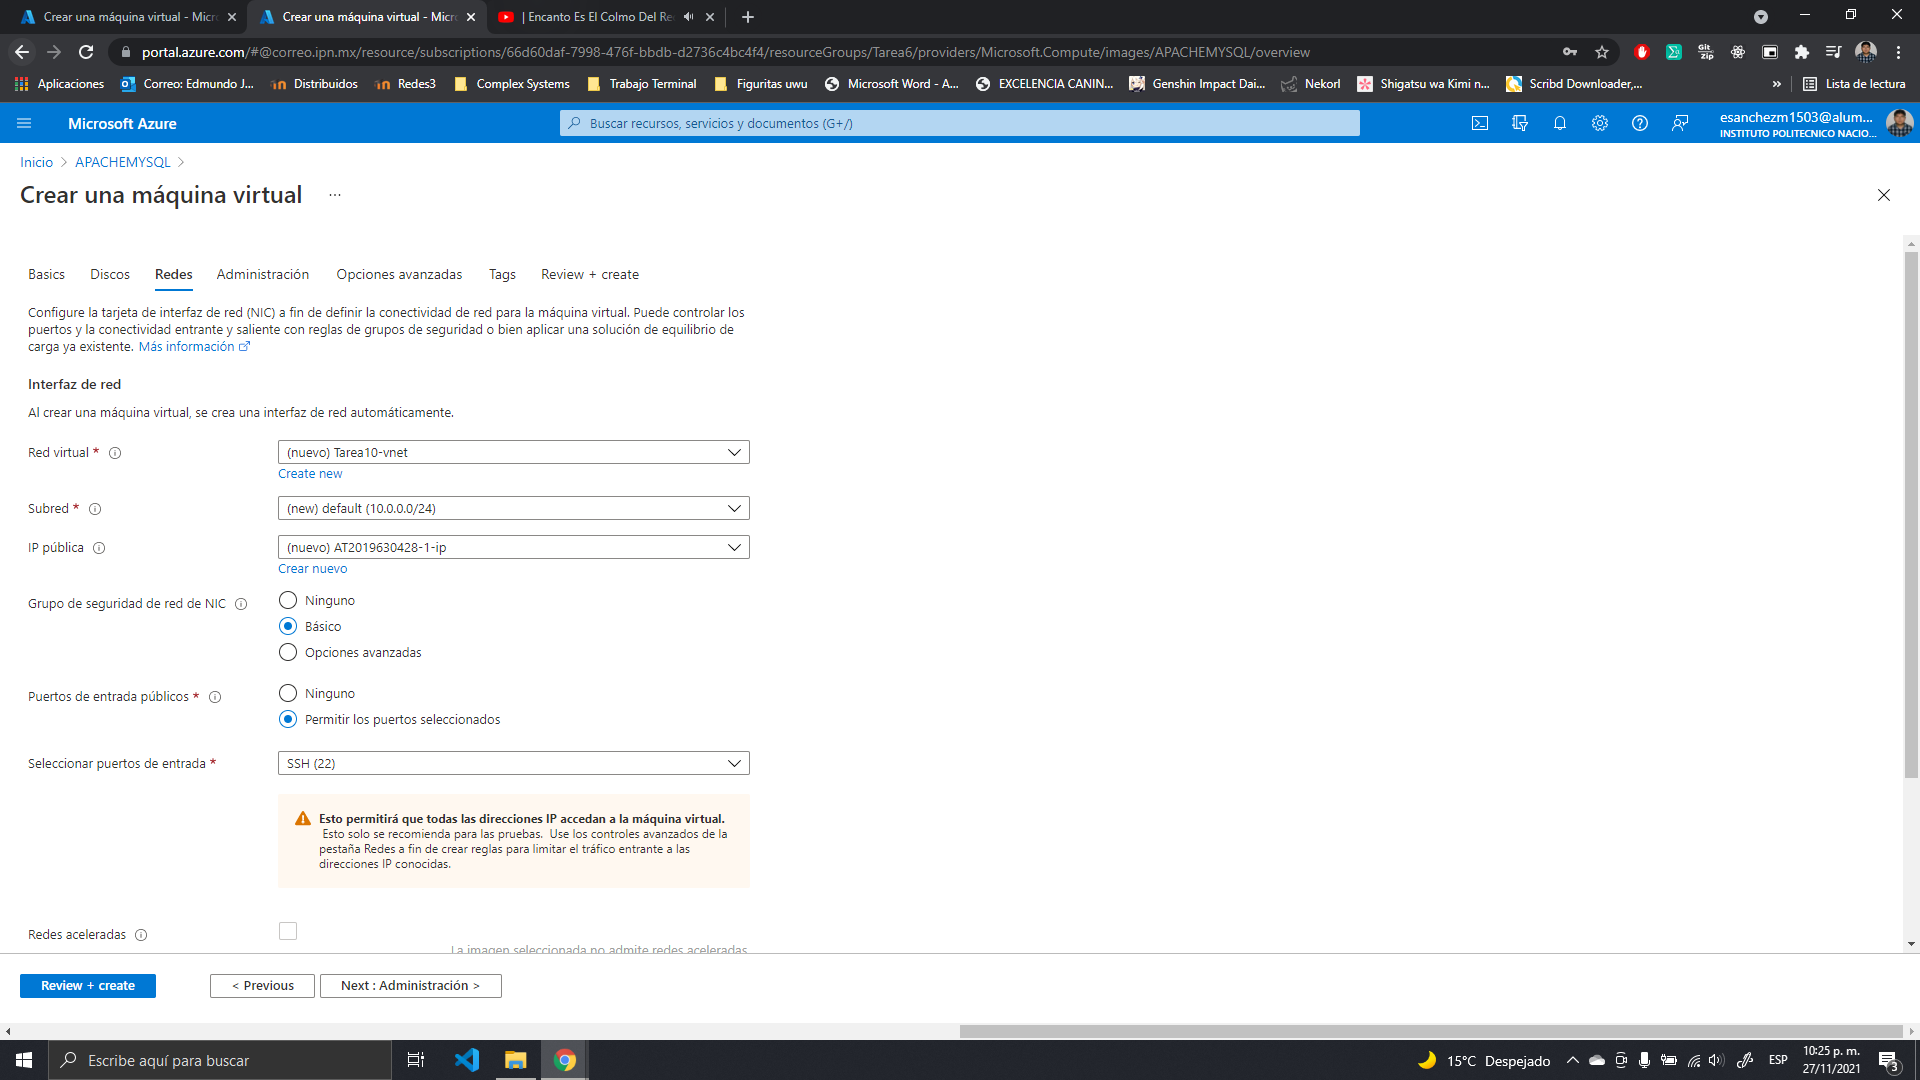
\includegraphics[scale=0.34]{resources/redes1.png}
			\caption{Información sobre la redes de la maquina virtual.}\label{fig:picture}
		\end{figure}
		\begin{figure}[H]
			\centering
			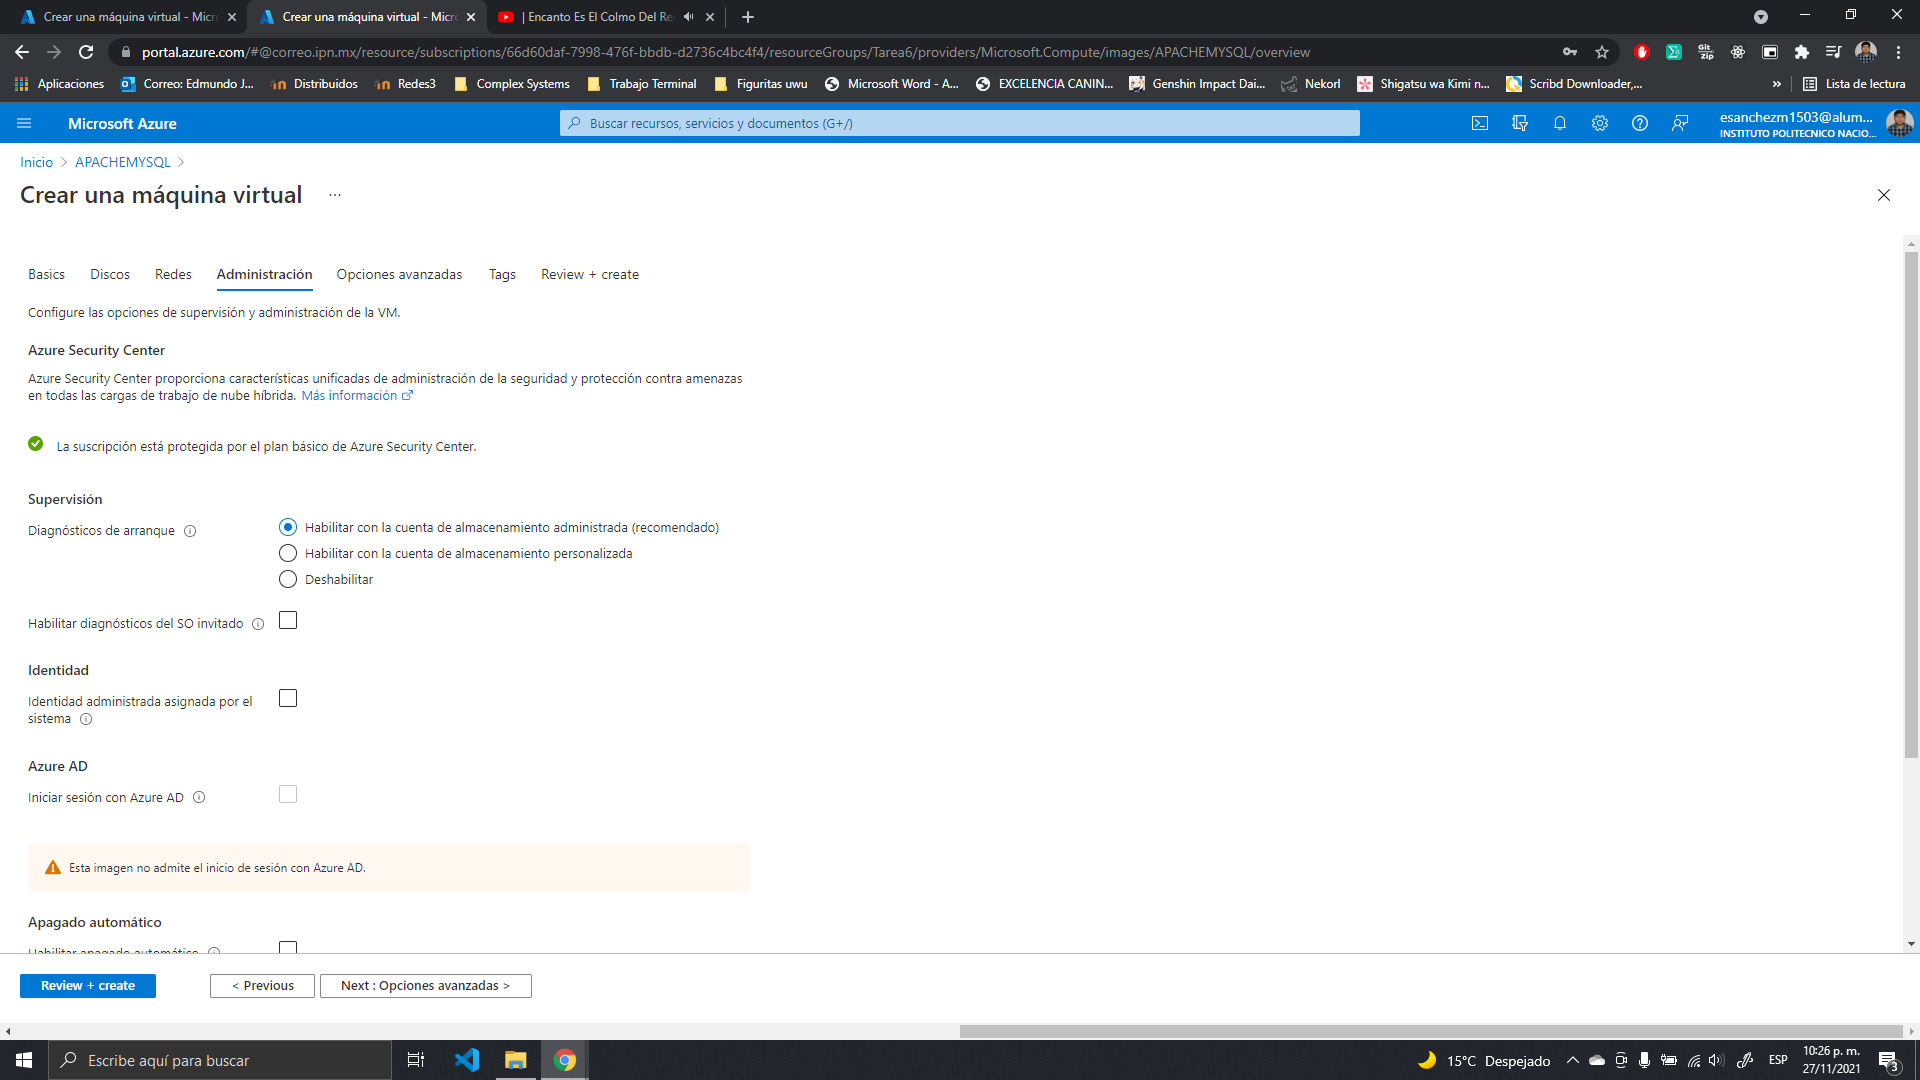
\includegraphics[scale=0.34]{resources/admin1.png}
			\caption{Configuración de la administración de la maquina virtual.}\label{fig:picture}
		\end{figure}
		\begin{figure}[H]
			\centering
			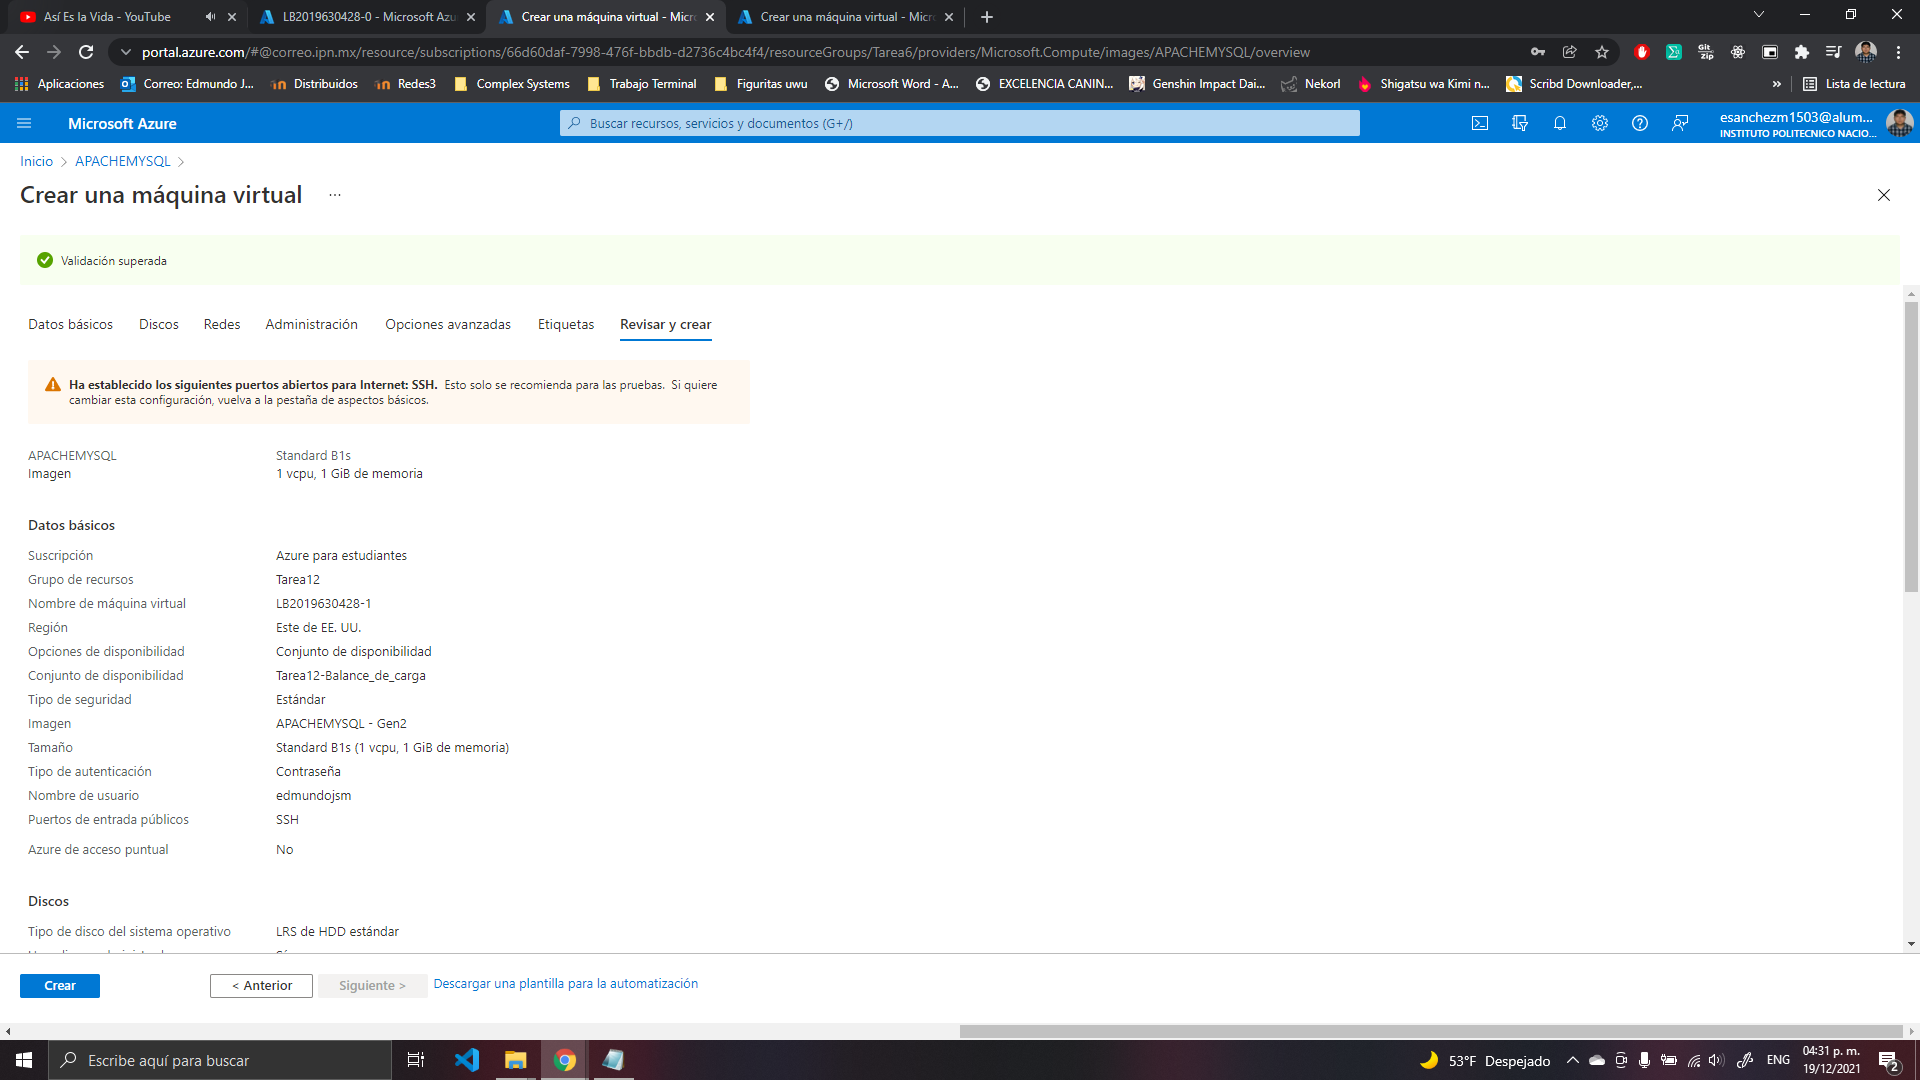
\includegraphics[scale=0.34]{resources/revisarycrear1.png}
			\caption{Creación de la maquina virtual.}\label{fig:picture}
		\end{figure}
		\begin{figure}[H]
			\centering
			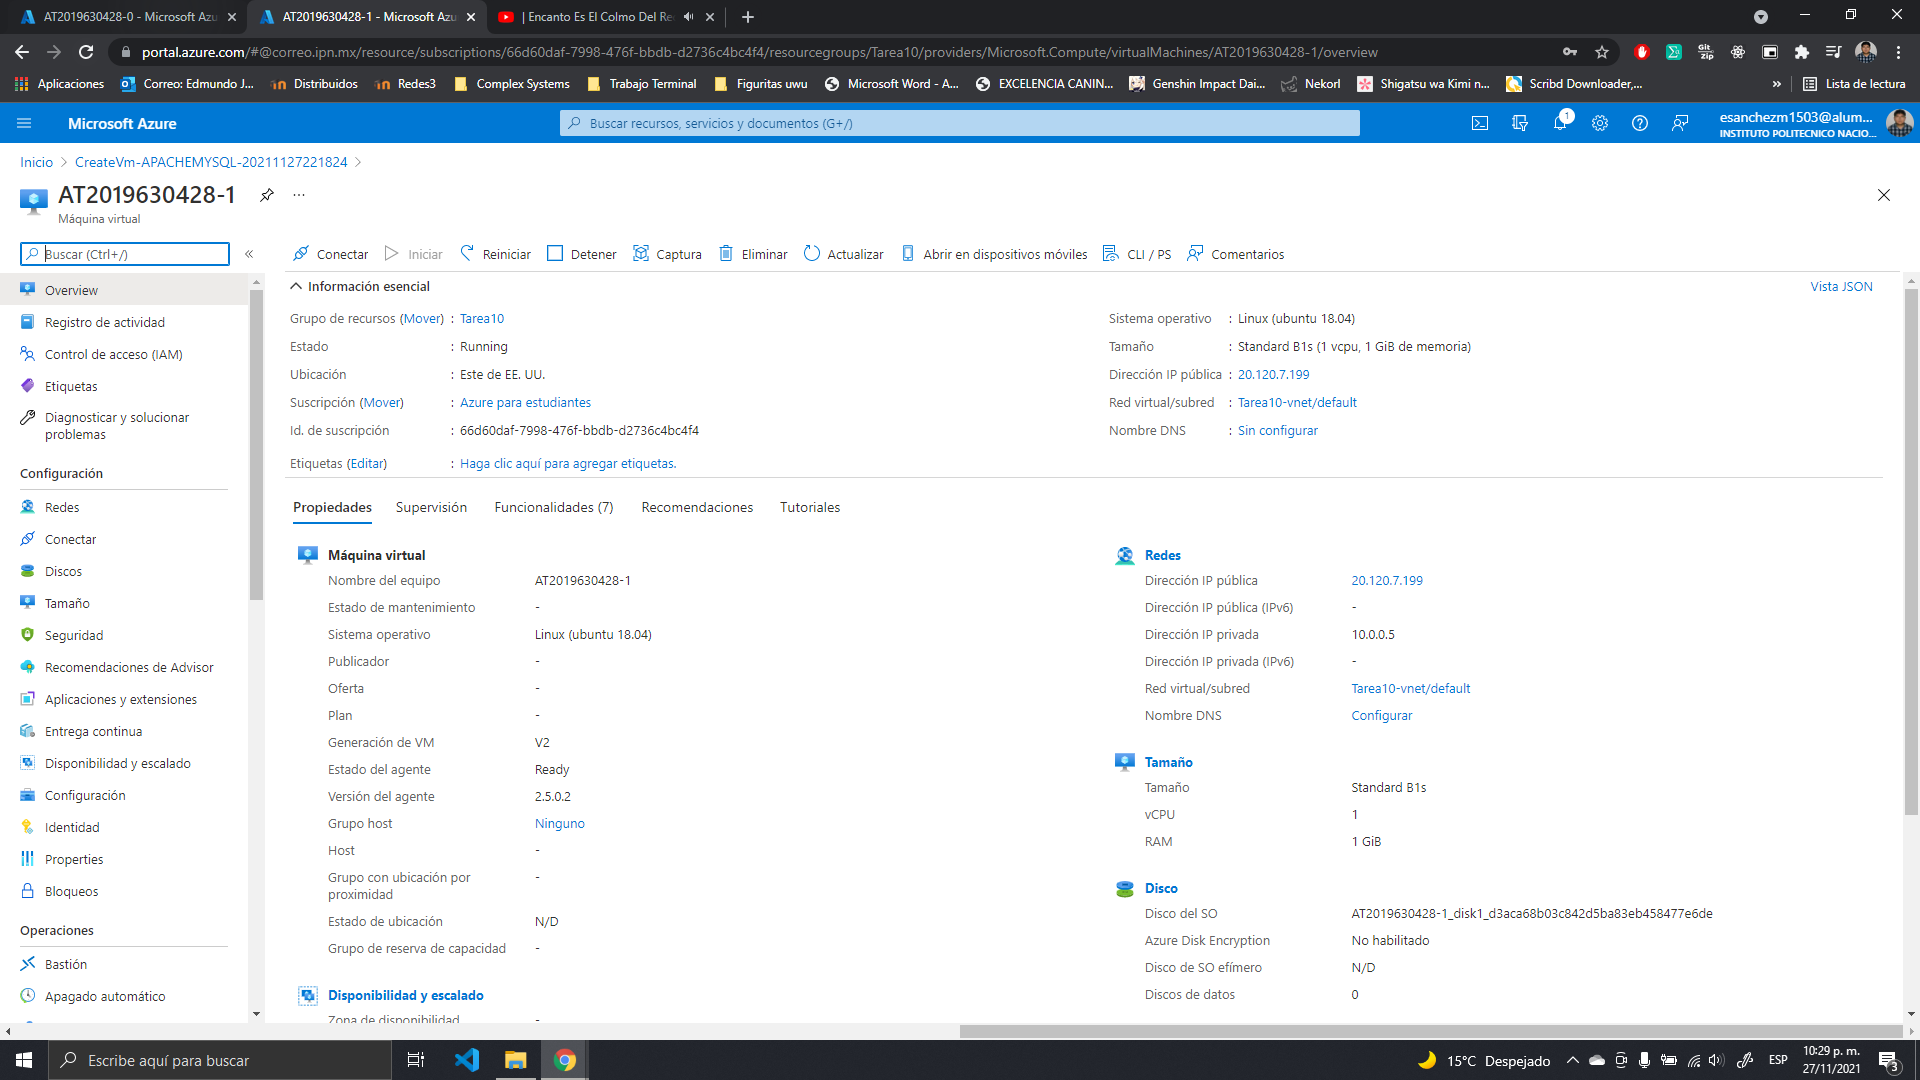
\includegraphics[scale=0.34]{resources/paneldecontrol1.png}
			\caption{Panel de control de la maquina virtual.}\label{fig:picture}
		\end{figure}
		Una vez creada la maquina virtual tenemos que abrir el puerto 8080, poniendo la IP de la maquina virtual 0 ya que sera la única computadora que va a poder acceder a esta maquina virtual.
		\begin{figure}[H]
			\centering
			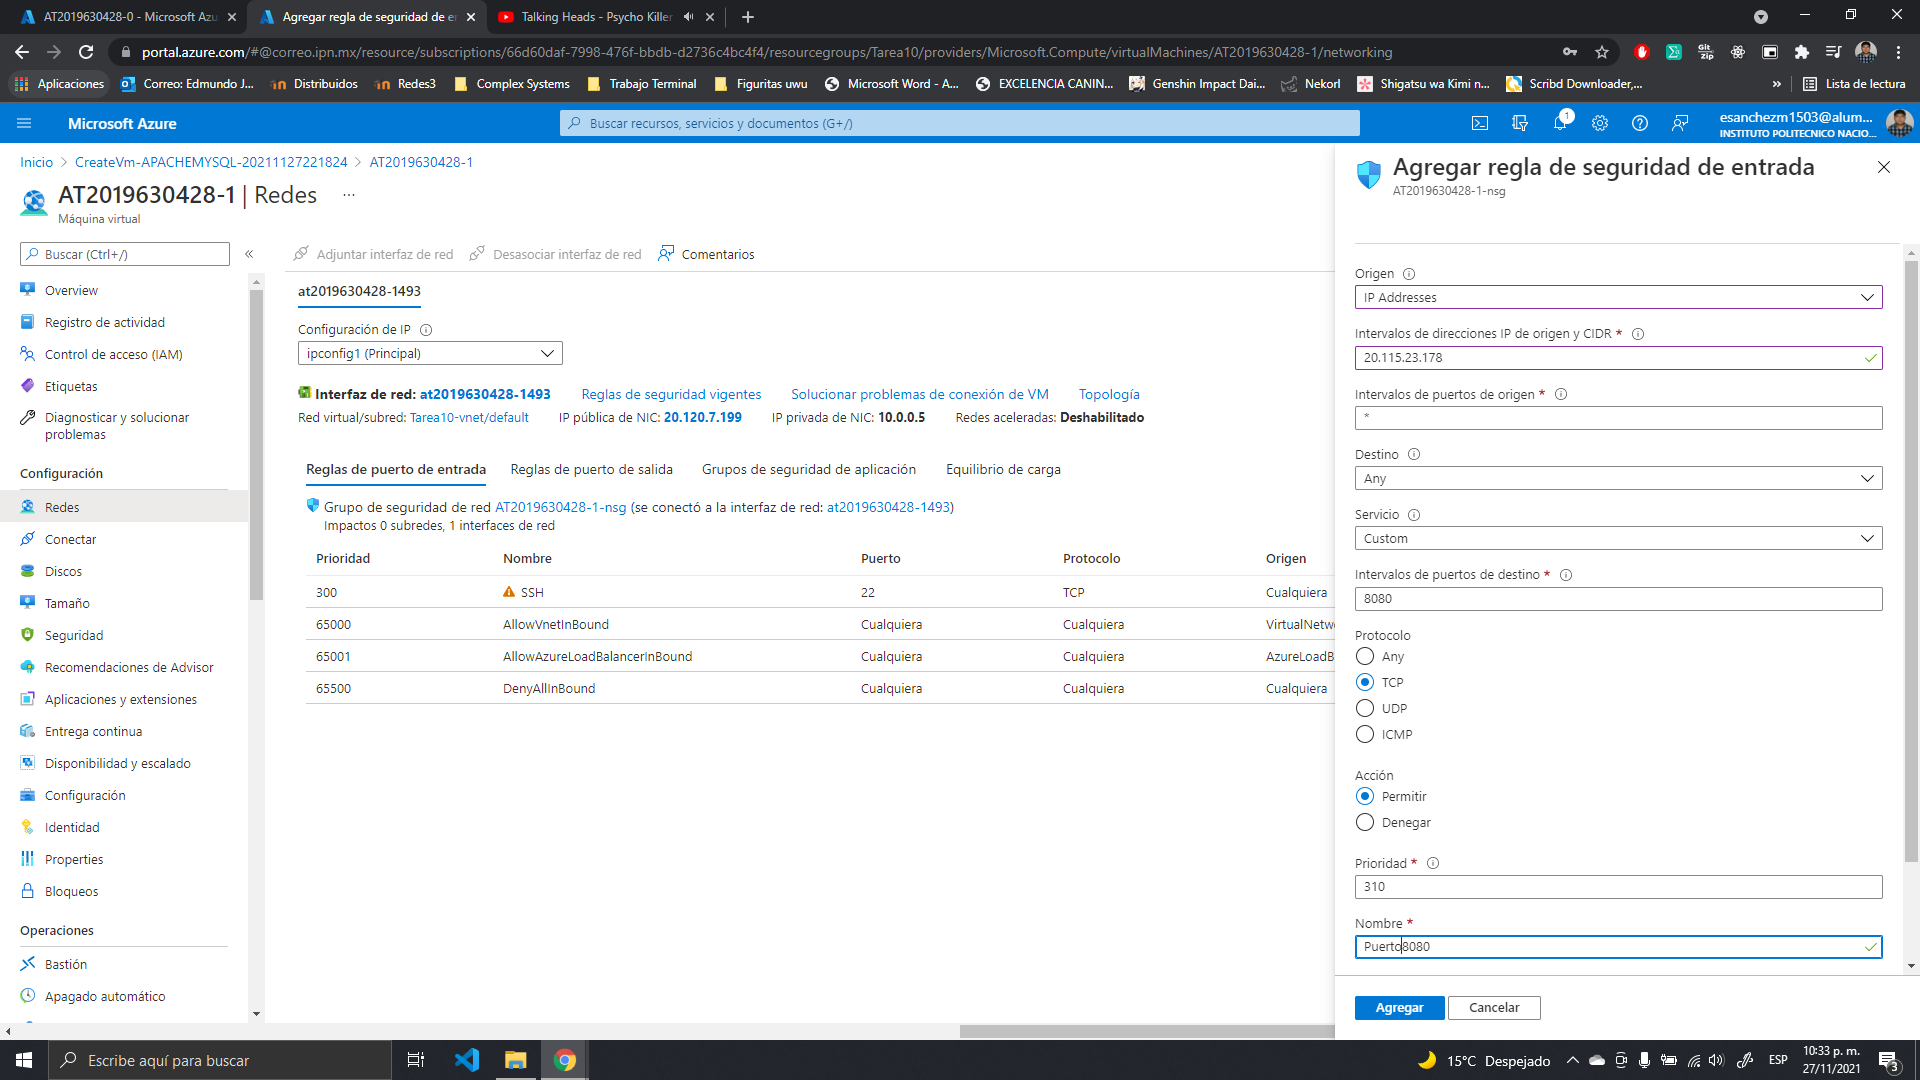
\includegraphics[scale=0.34]{resources/puerto80801.png}
			\caption{Configuración del puerto 8080.}\label{fig:picture}
		\end{figure}
		\begin{figure}[H]
			\centering
			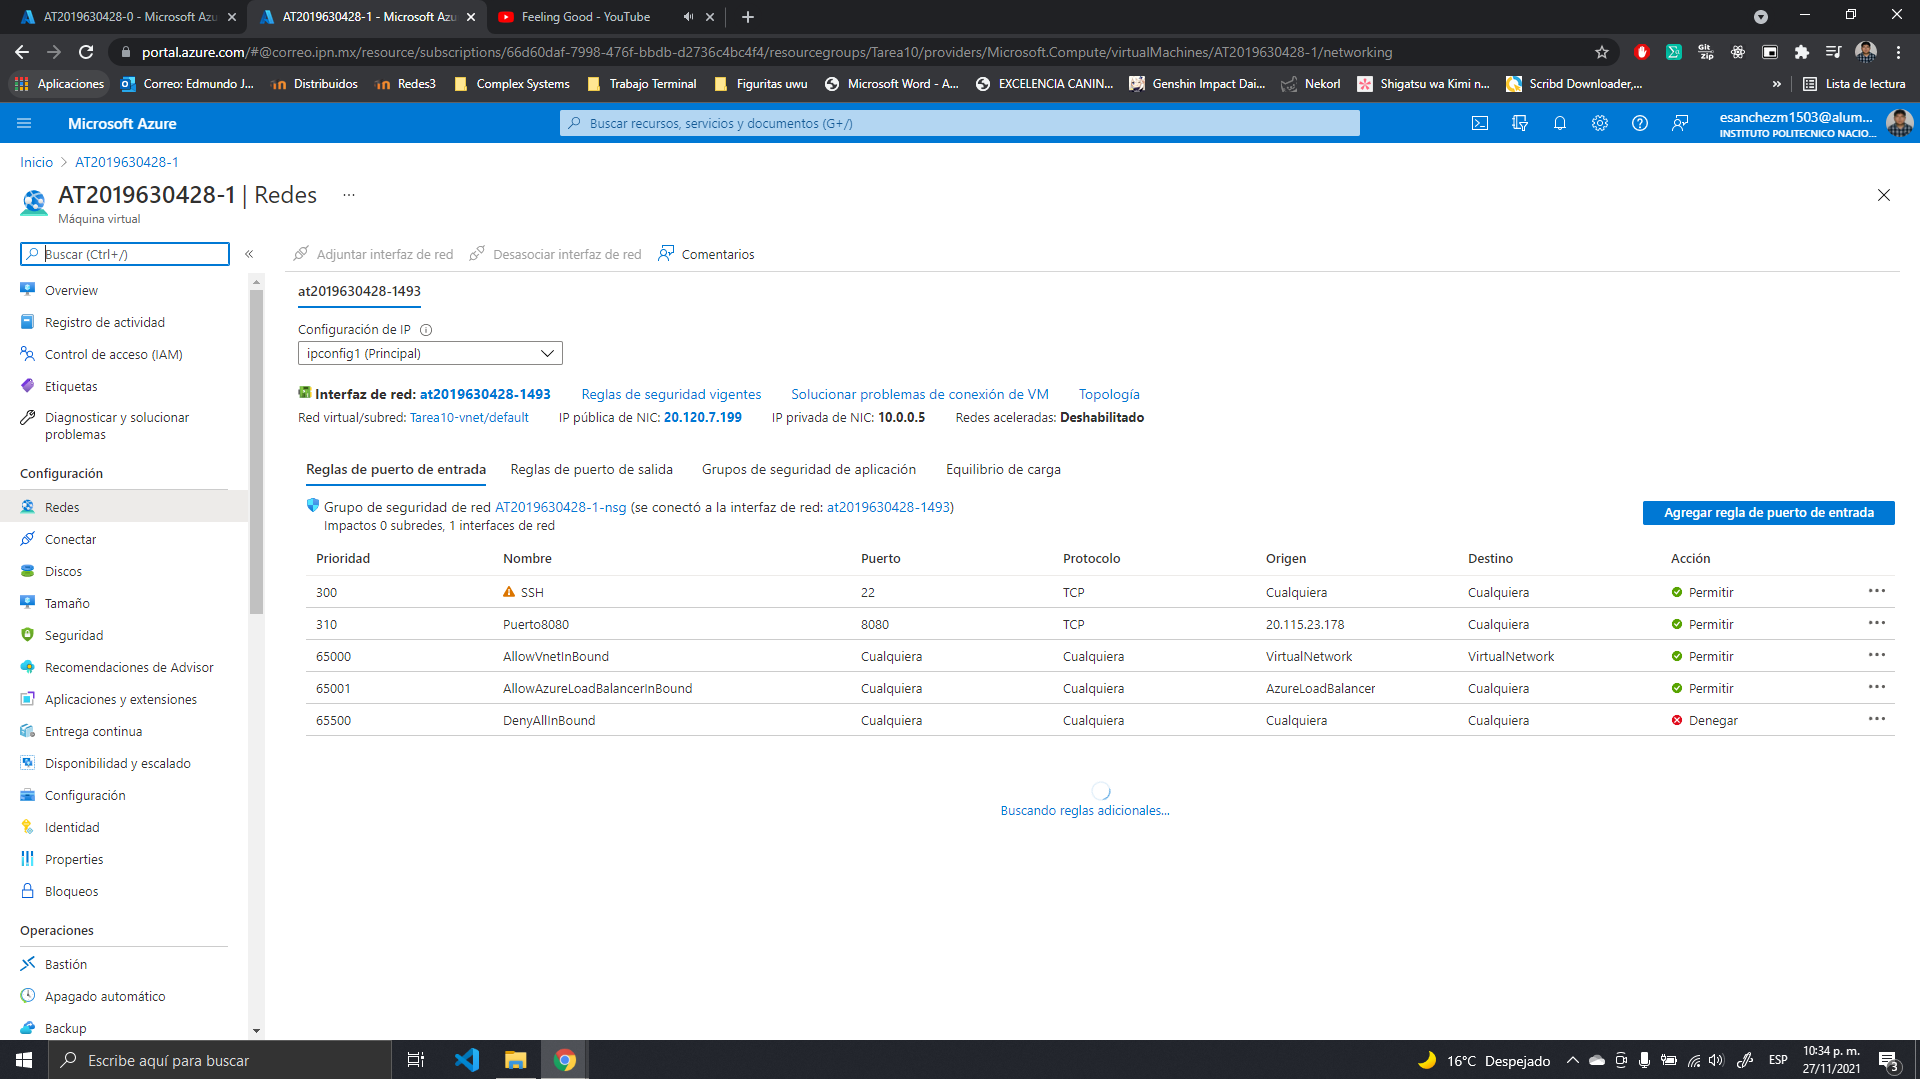
\includegraphics[scale=0.34]{resources/puertook1.png}
			\caption{Puerto 8080 abierto correctamente.}\label{fig:picture}
		\end{figure}
		\subsection{Conexión SSH con el sistema principal de manera exitosa}
		En esta parte veremos la conexión del equipo de computo utilizado con la maquina virtual que sera nuestro sistema principal	.
		\begin{figure}[H]
			\centering
			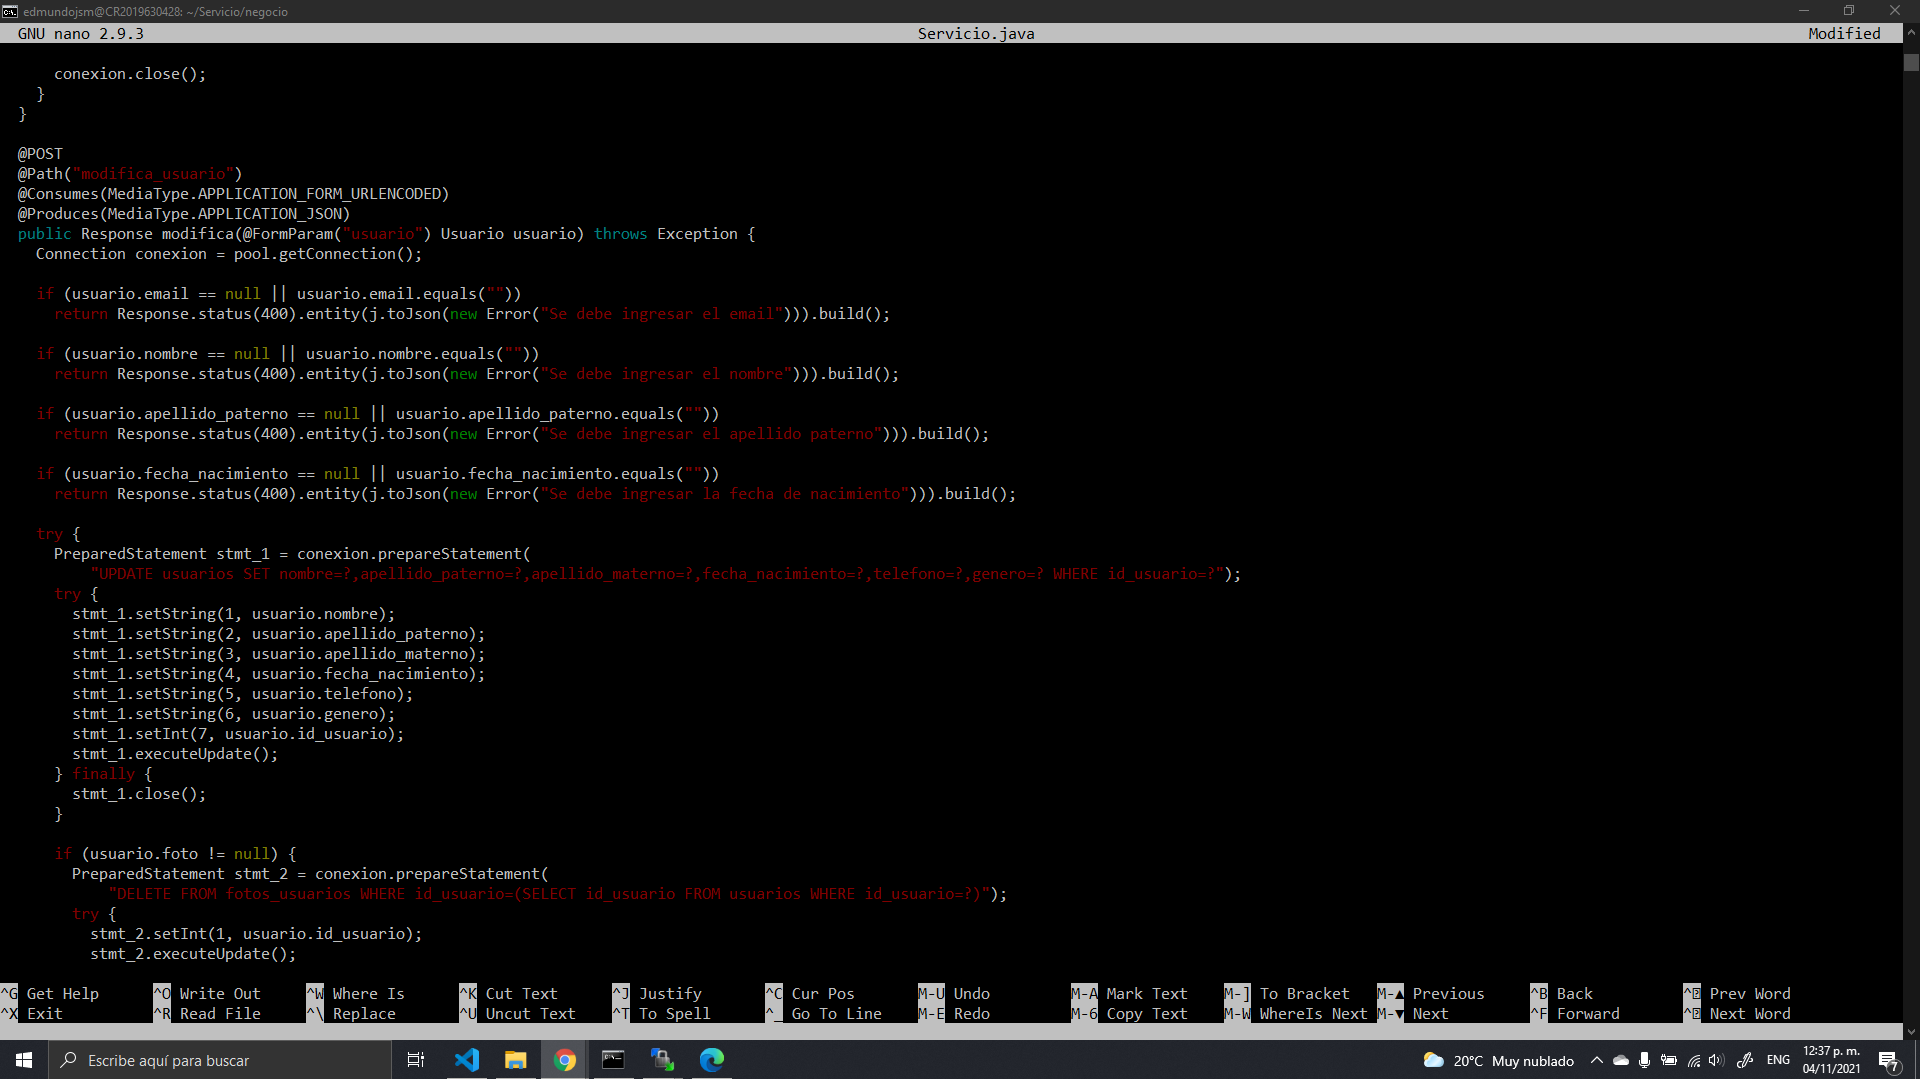
\includegraphics[scale=0.34]{resources/p4.png}
			\caption{Conexión con la maquina virtual que sera nuestro sistema principal.}\label{fig:picture}
		\end{figure}
		\subsection{Utilizando el programa sftp enviar a la máquina virtual 0 (sistema principal) el archivo: SimpleProxyServer.java}
		En esta parte veremos el uso de sftp para el envió de archivos entre maquina local con la maquina virtual del Sistema principal.\par
		La forma de usar sftp es muy simple, sin embargo, nunca había hecho uso de este protocolo, por eso como vemos en la figura 18 vemos que en la primera linea no funciono, pero investigando un poco mas lo mas fácil era hacer conexión primero con sftp que es como hacer conexión usando ssh, una vez conectado hacemos uso de put para enviar el archivo y mandamos la ruta absoluta del archivo y con el comando ls en la conexión sftp y vemos como el archivo ya esta en la maquina virtual.
		\begin{figure}[H]
			\centering
			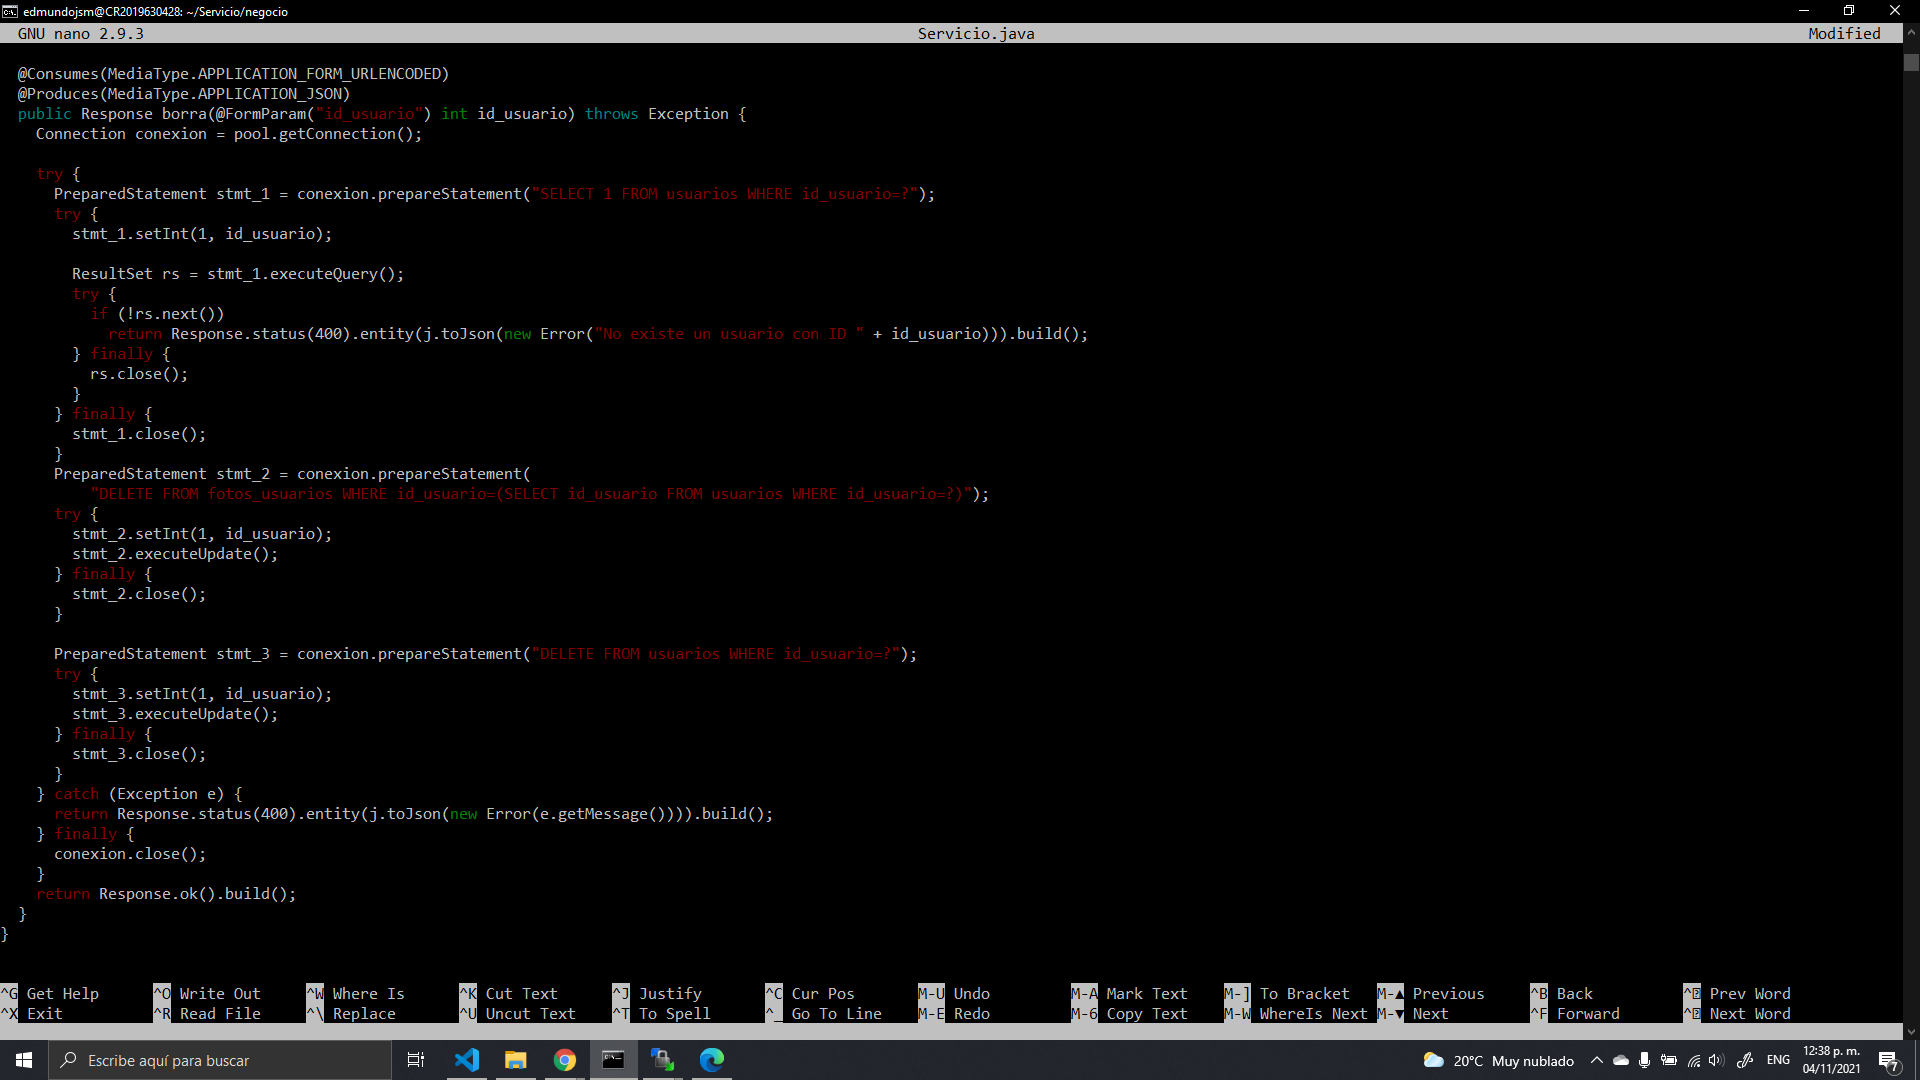
\includegraphics[scale=0.34]{resources/p5.png}
			\caption{Copia del archivo SimpleProxyServer.java al sistema principal.}\label{fig:picture}
		\end{figure}
		\subsection{Compilar en la máquina virtual 0 (sistema principal) el programa SimpleProxyServer.java}
		En esta parte veremos la compilación del archivo que pasamos en el paso anterior, ademas de verificar de que el archivo si se copio y que ademas la compilación se desarrollo de manera exitosa.
		\begin{figure}[H]
			\centering
			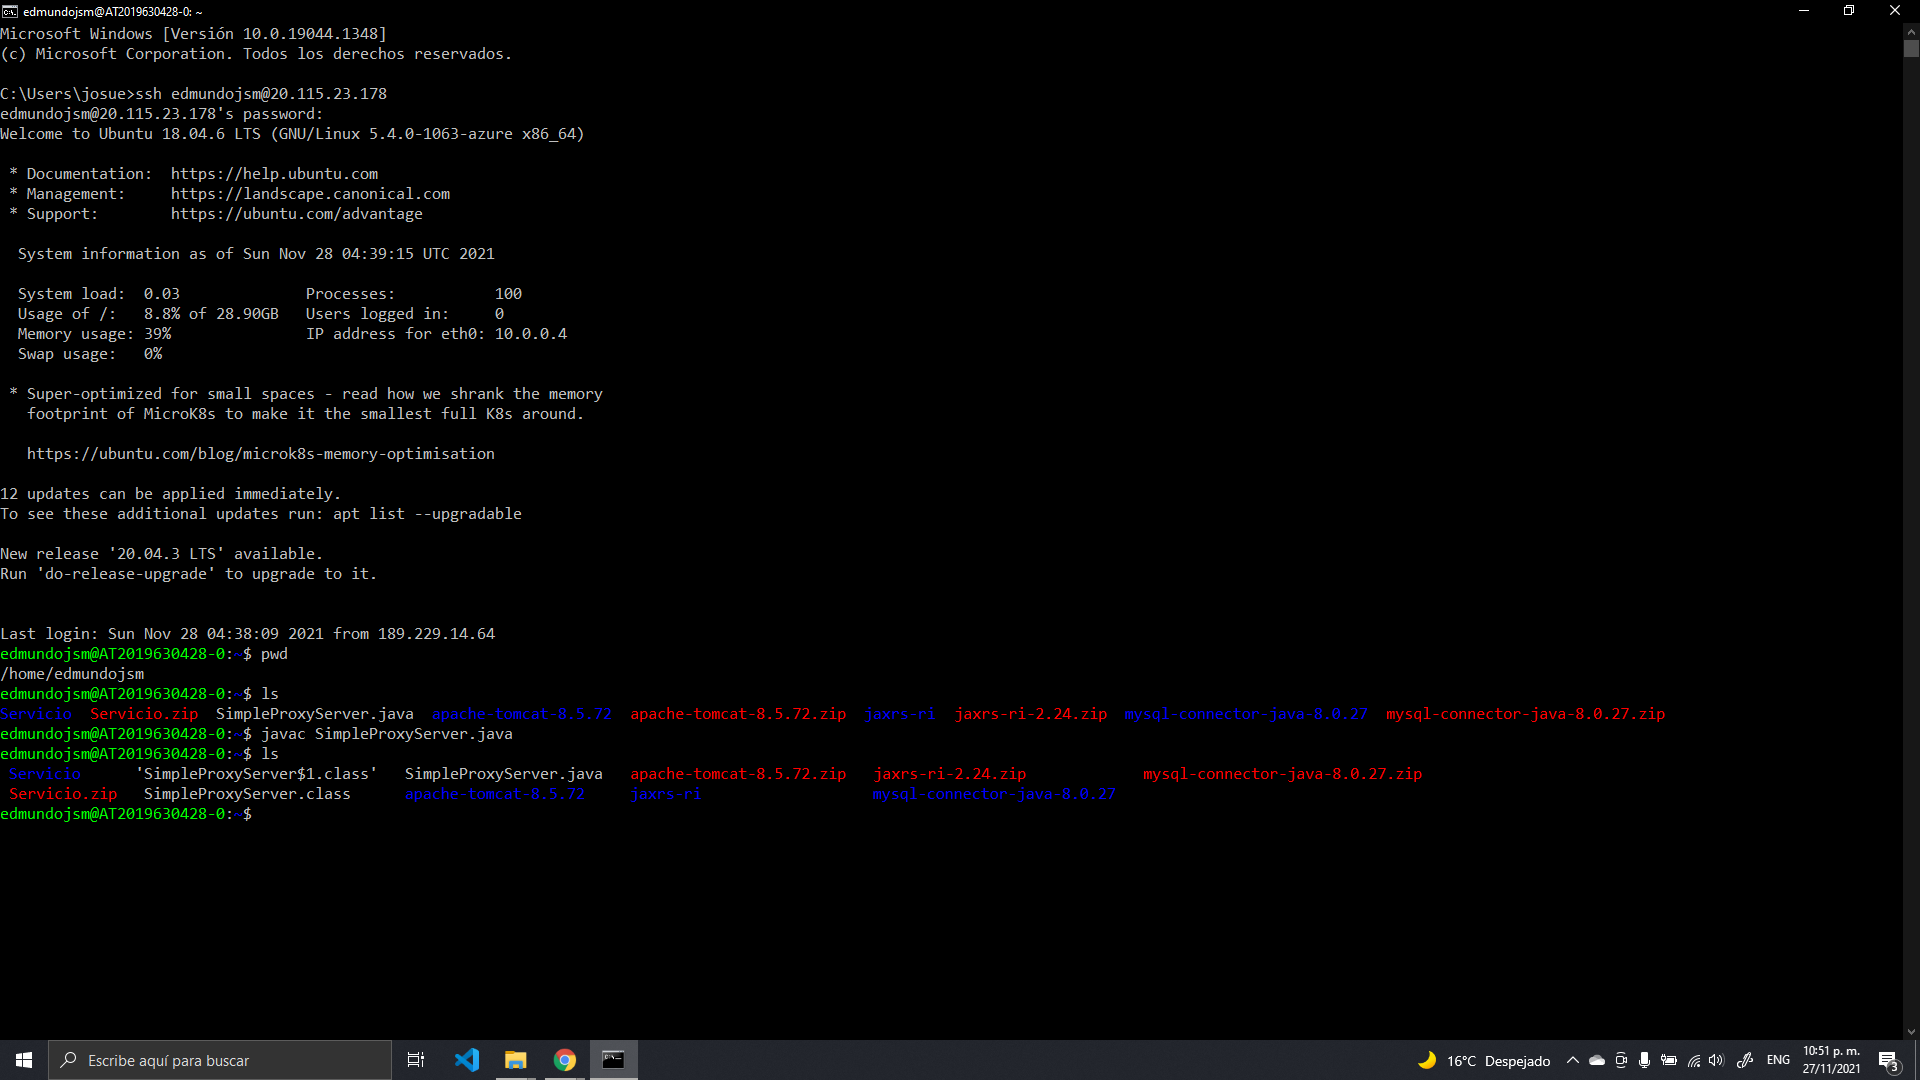
\includegraphics[scale=0.34]{resources/p6.png}
			\caption{Compilación del archivo SimpleProxyServer.java.}\label{fig:picture}
		\end{figure}
		\subsection{Iniciar Tomcat en las máquinas virtuales 0 y 1 (sistema principal y sistema replica).}
		En esta parte veremos el inicio de Tomcat en ambas maquinas virtuales, en la figura 20 están la ambas conexiones, del lado derecho esta el sistema principal y del lado izquierdo esta el sistema replica y vemos como el inicio de Tomcat se realizo correctamente.
		\begin{figure}[H]
			\centering
			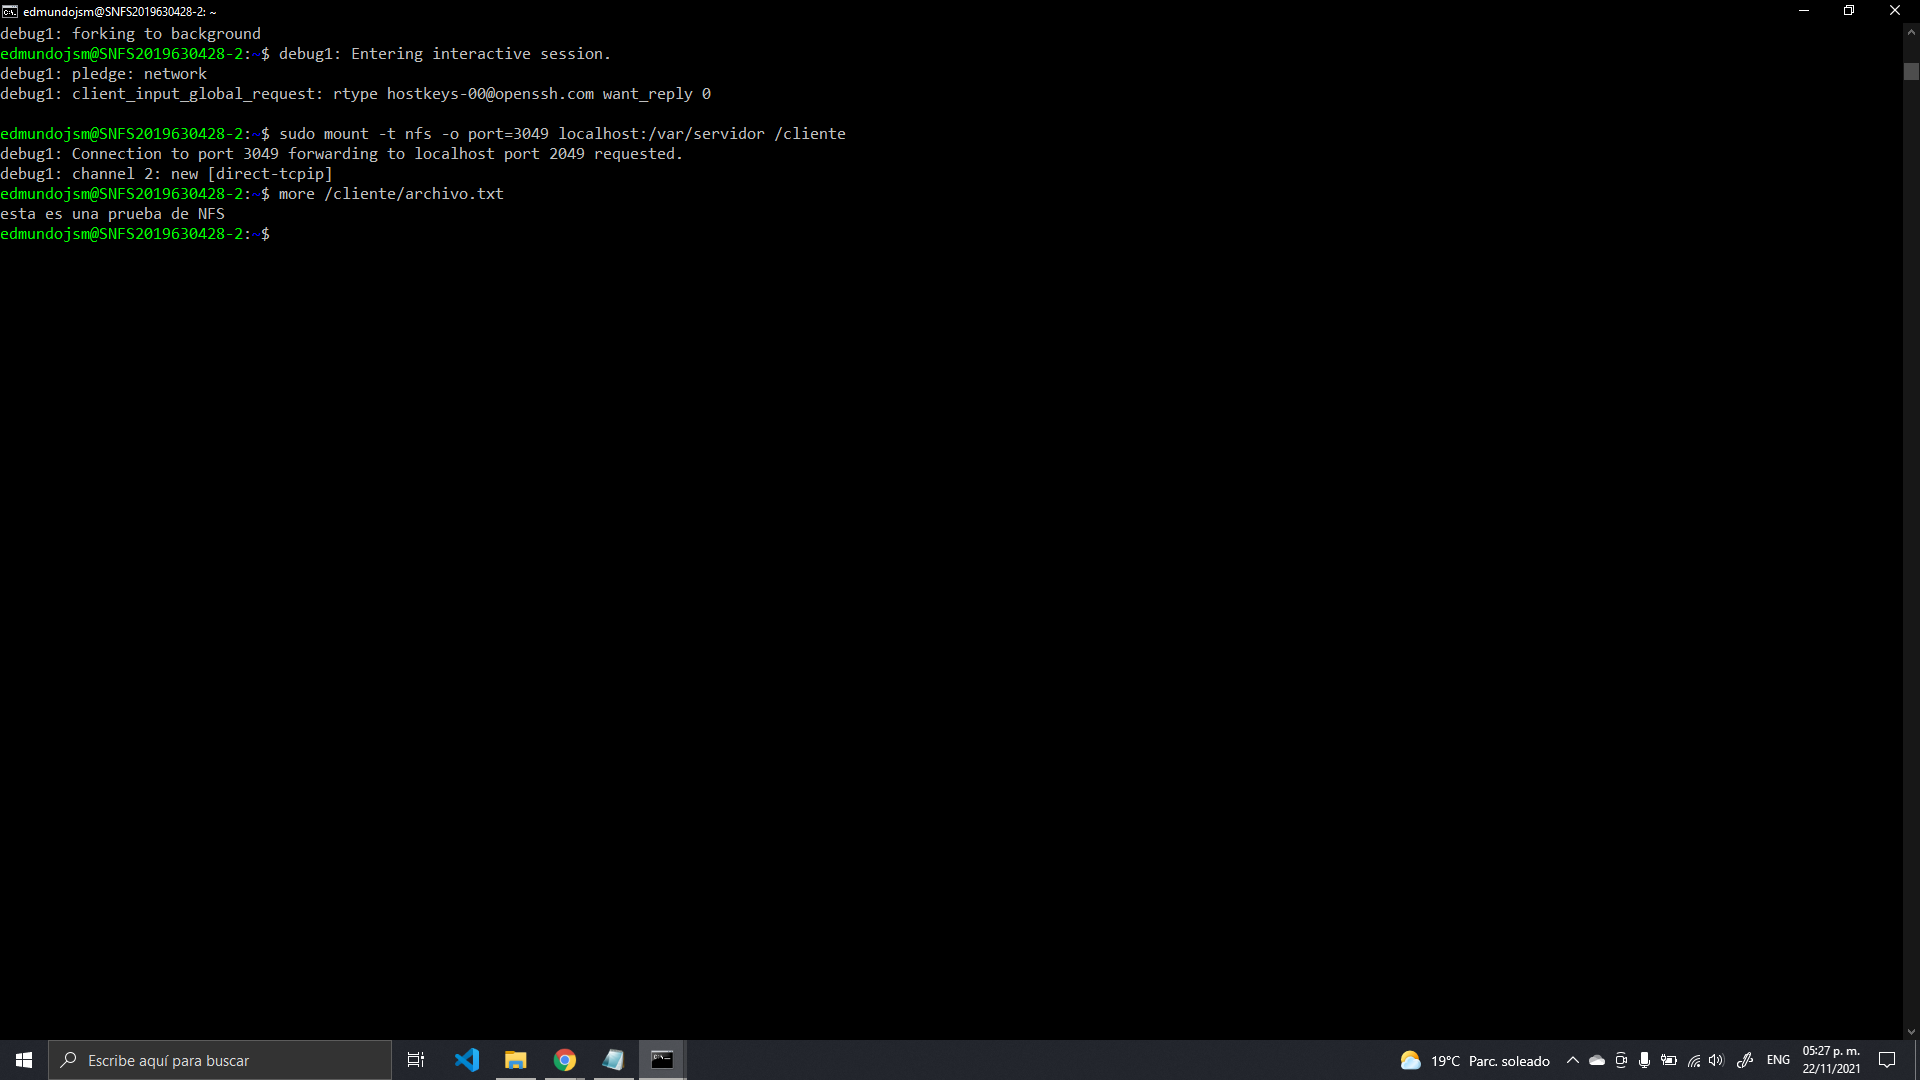
\includegraphics[scale=0.34]{resources/p7.png}
			\caption{Inicio de Tomcat en ambas maquinas virtuales.}\label{fig:picture}
		\end{figure}
		\subsection{Ejecutar el máquina virtual 1 el proxy: sudo java SimpleProxyServer ip-maquina-virtual-2 8080 80 8080 \&}
		En esta parte veremos la ejecución de SimpleProxyServer, el comando que esta disponible en la plataforma es incorrecto ya que tiene un parámetro extra el cual es \&, lo único que tendríamos que modificar seria borrar \& y con eso el programa funciona correctamente, por lo que el comando seria el siguiente.
		\begin{verbatim}
			sudo java SimpleProxyServer ip-maquina-virtual-2 8080 80 8080
		\end{verbatim}
		Finalmente mencionar que como vemos en la figura 21 la primera linea no funciona correctamente el programa y en la segunda nos aparece el mensaje de que se inicio el programa de manera exitosa, mencionar que para las siguientes prueba abrí una nueva venta de linea de comando para poder realizar lo solicitado en la practica ya que este programa queda activo y nos deja utilizar la linea de comando
		\begin{figure}[H]
			\centering
			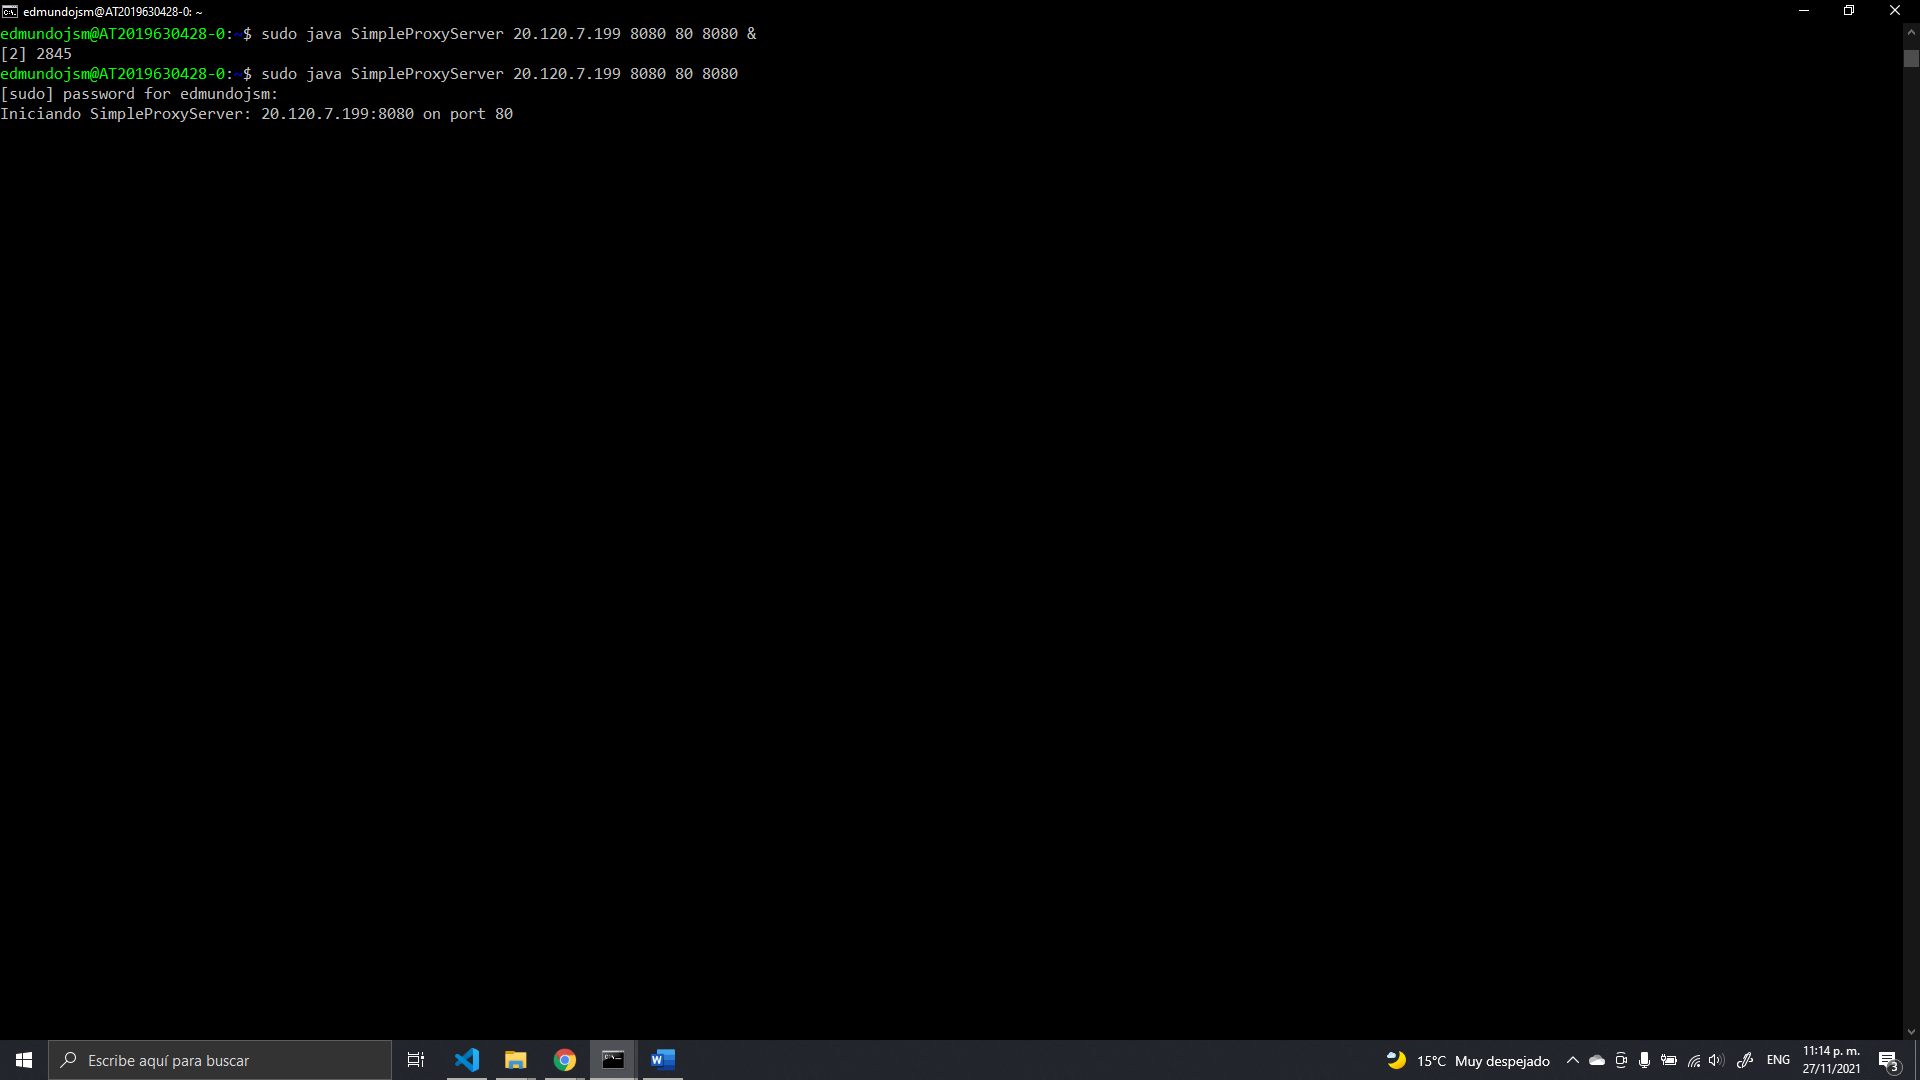
\includegraphics[scale=0.34]{resources/p8.png}
			\caption{Ejecución de programa de manera exitosa.}\label{fig:picture}
		\end{figure}
		\subsection{Ingresar la siguiente URL en un navegador, notar que no es necesario ingresar el nombre del puerto, ya que se utiliza el puerto default 80:}
		En esta parte veremos como el servicio funciona de manera correcta y ahora ya no necesitamos pasar el puerto para la conexión al servidor Tomcat, solo necesitamos hacer uso de la IP del sistema principal con el elemento a buscar en este caso prueba.html.
		\begin{figure}[H]
			\centering
			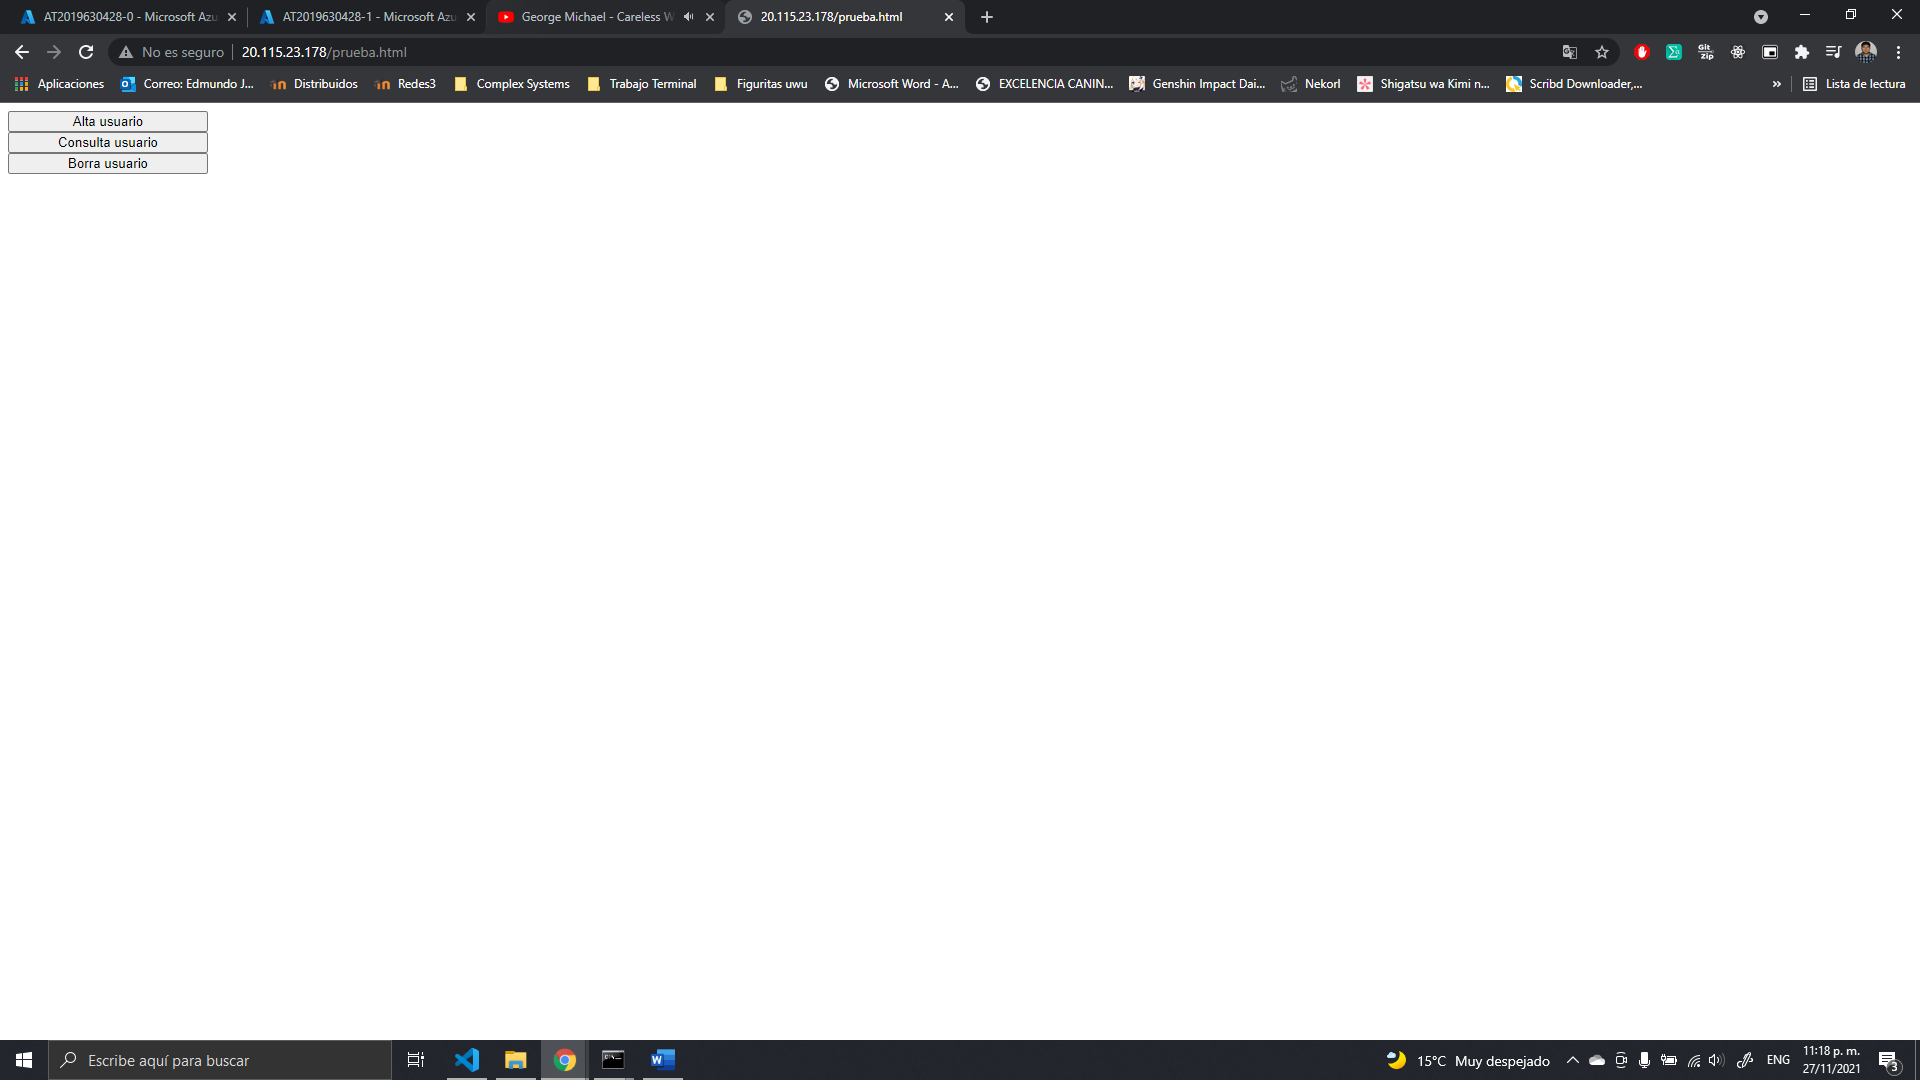
\includegraphics[scale=0.34]{resources/p9.png}
			\caption{Sistema REST funcionando de manera exitosa.}\label{fig:picture}
		\end{figure}
		\subsection{Dar clic en el botón ``Alta usuario'' para dar de alta un nuevo usuario. Capturar los campos y dar clic en el botón ``Alta''.}
		Antes de ir directamente a la prueba veremos algo curioso y es que al crear la imagen su guarda todo lo que teníamos y teníamos almacenado una prueba del sistema y como vemos en la figura 23, sigue guardada la prueba.
		\begin{figure}[H]
			\centering
			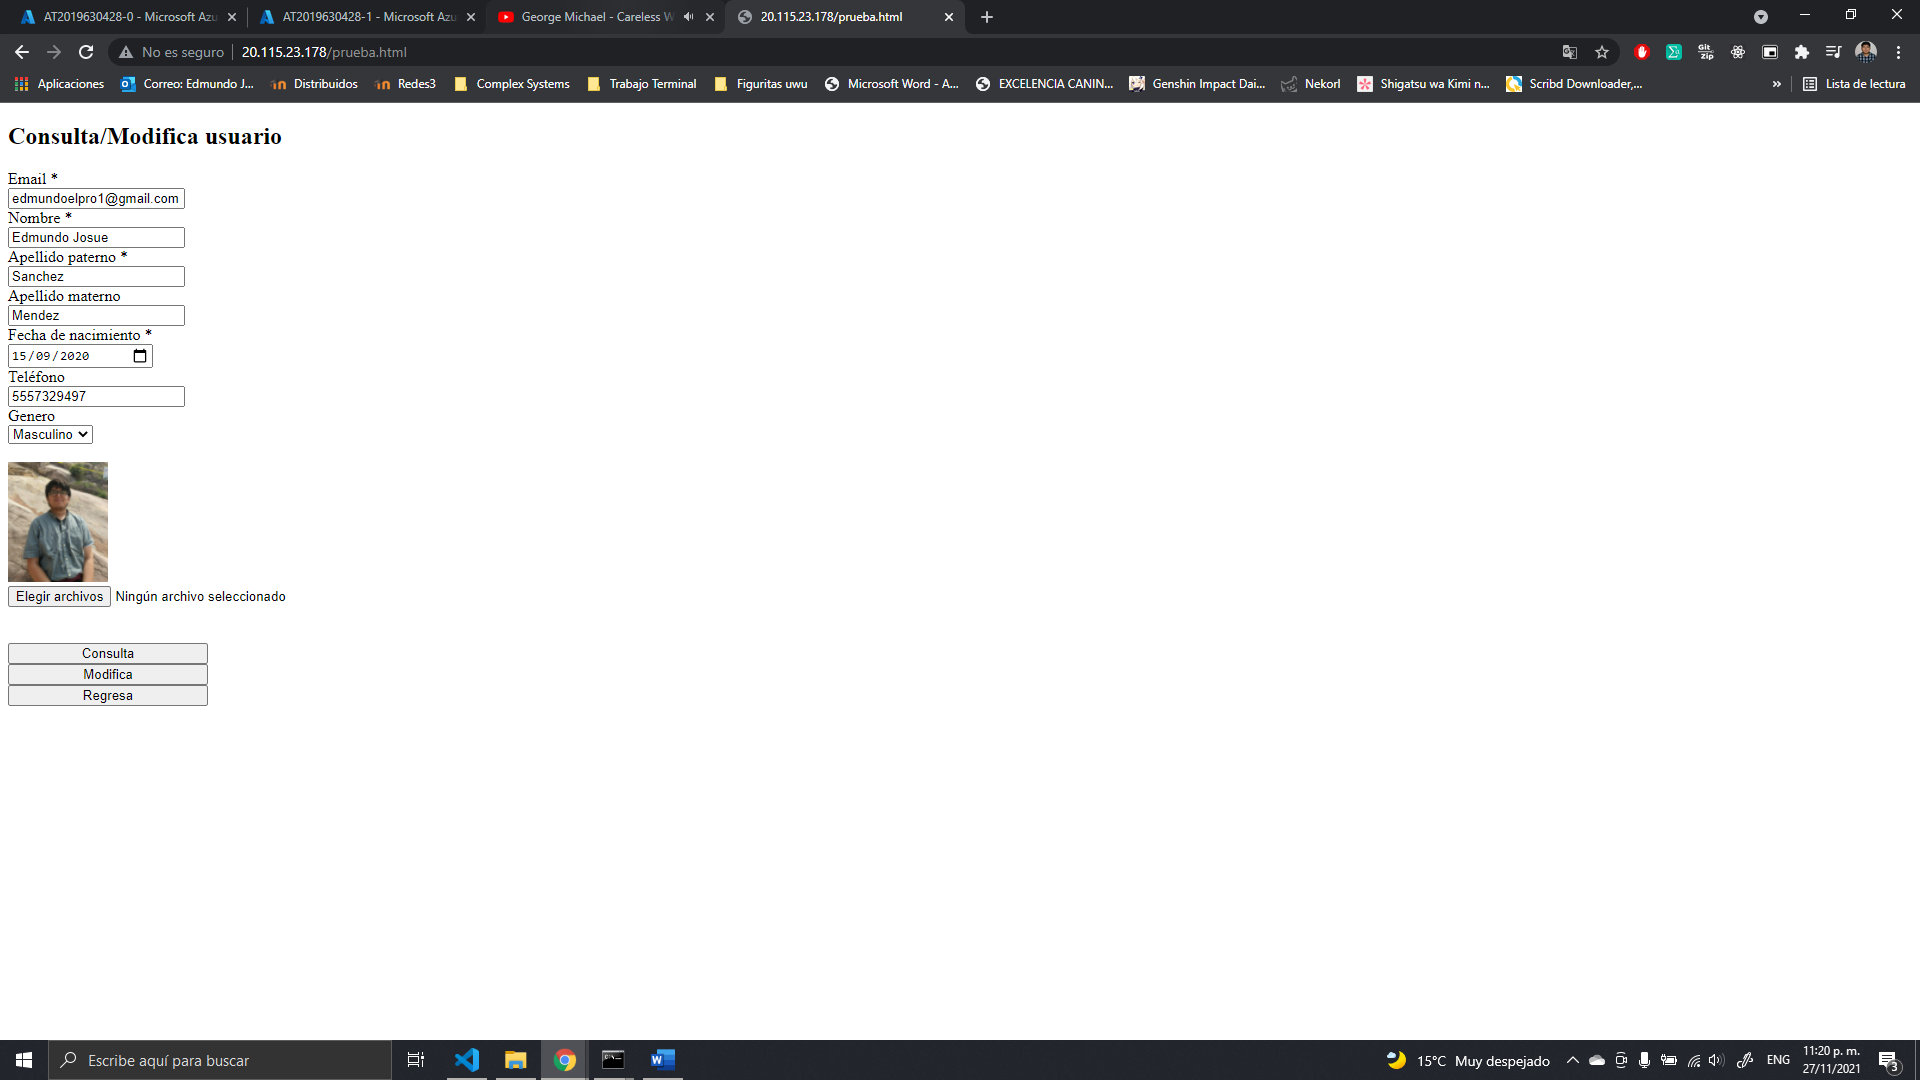
\includegraphics[scale=0.34]{resources/previo.png}
			\caption{Sistema con datos almacenados previamente.}\label{fig:picture}
		\end{figure}
		Ahora en la figura 24 y 25 podemos ver como en la pagina se da alta de usuario de manera correcta
		\begin{figure}[H]
			\centering
			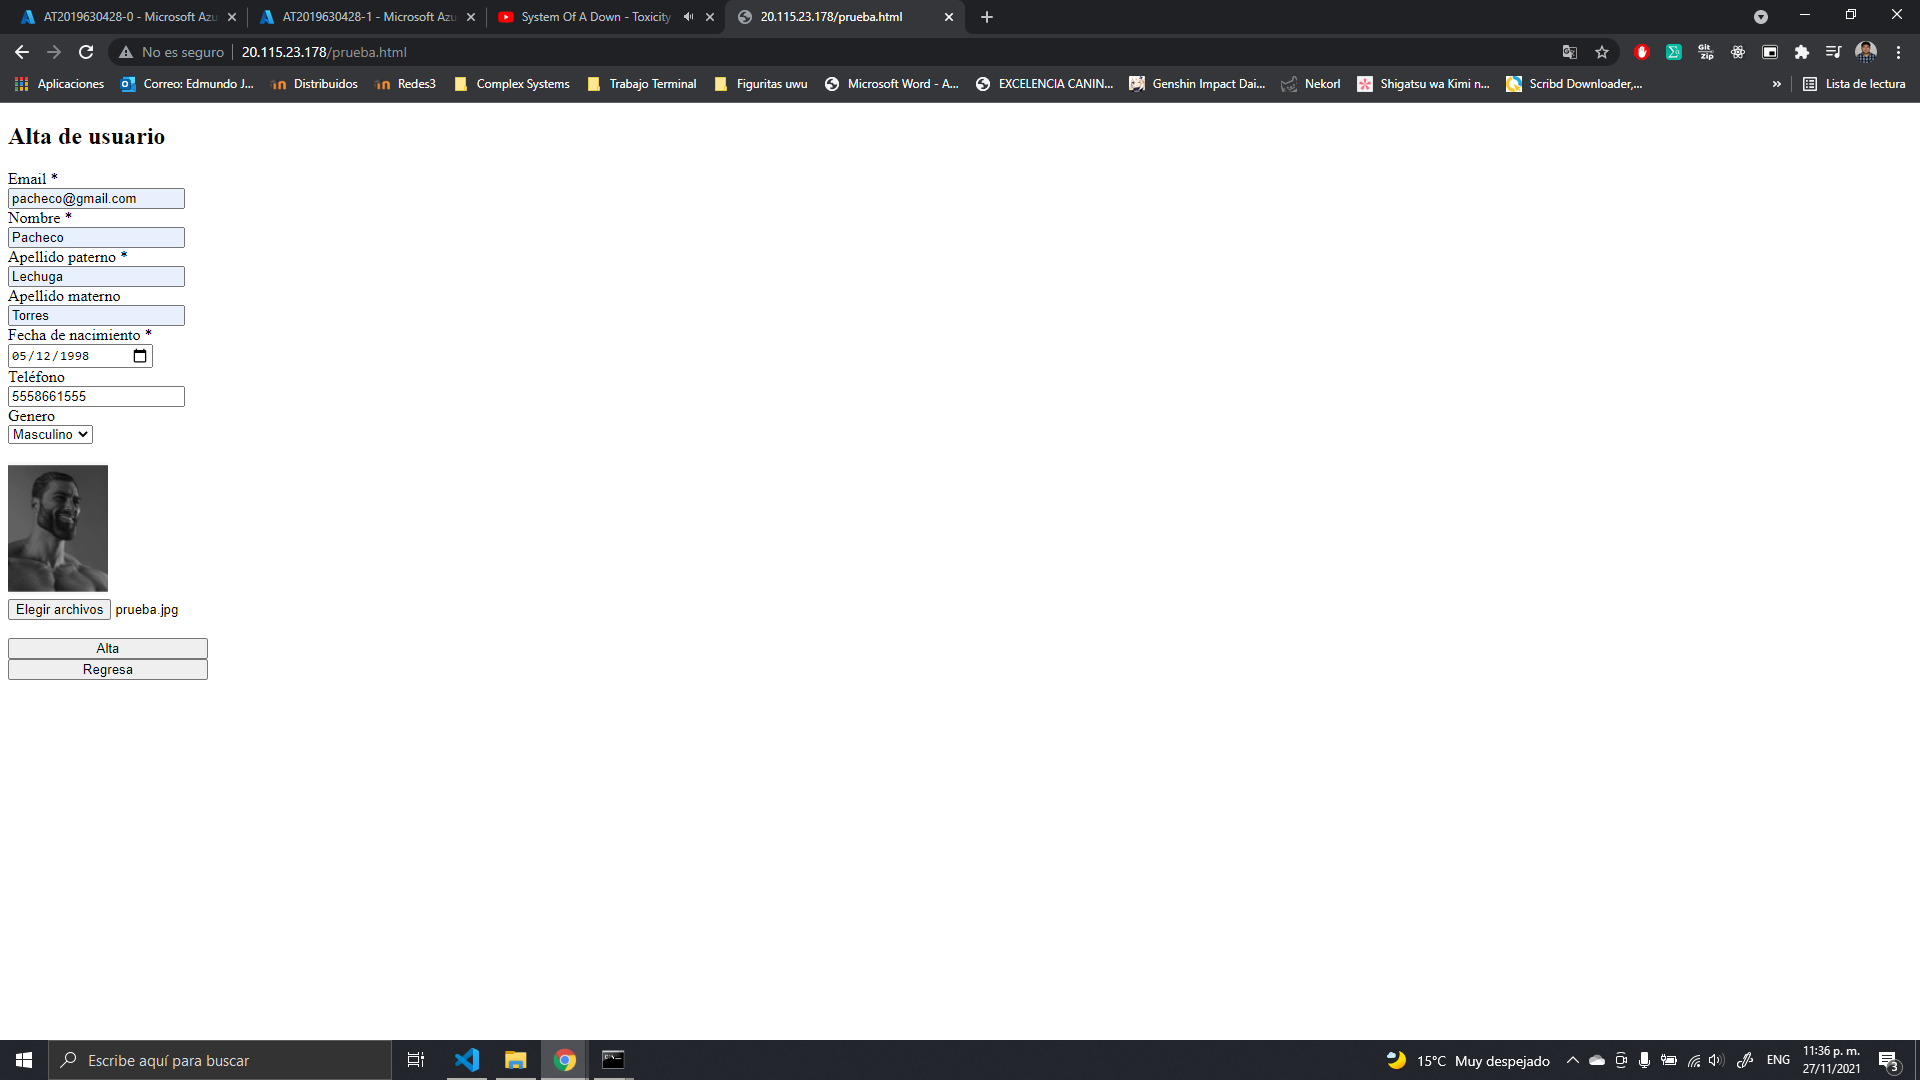
\includegraphics[scale=0.34]{resources/p9.2.png}
			\caption{Alta de usuario.}\label{fig:picture}
		\end{figure}	
		\begin{figure}[H]
			\centering
			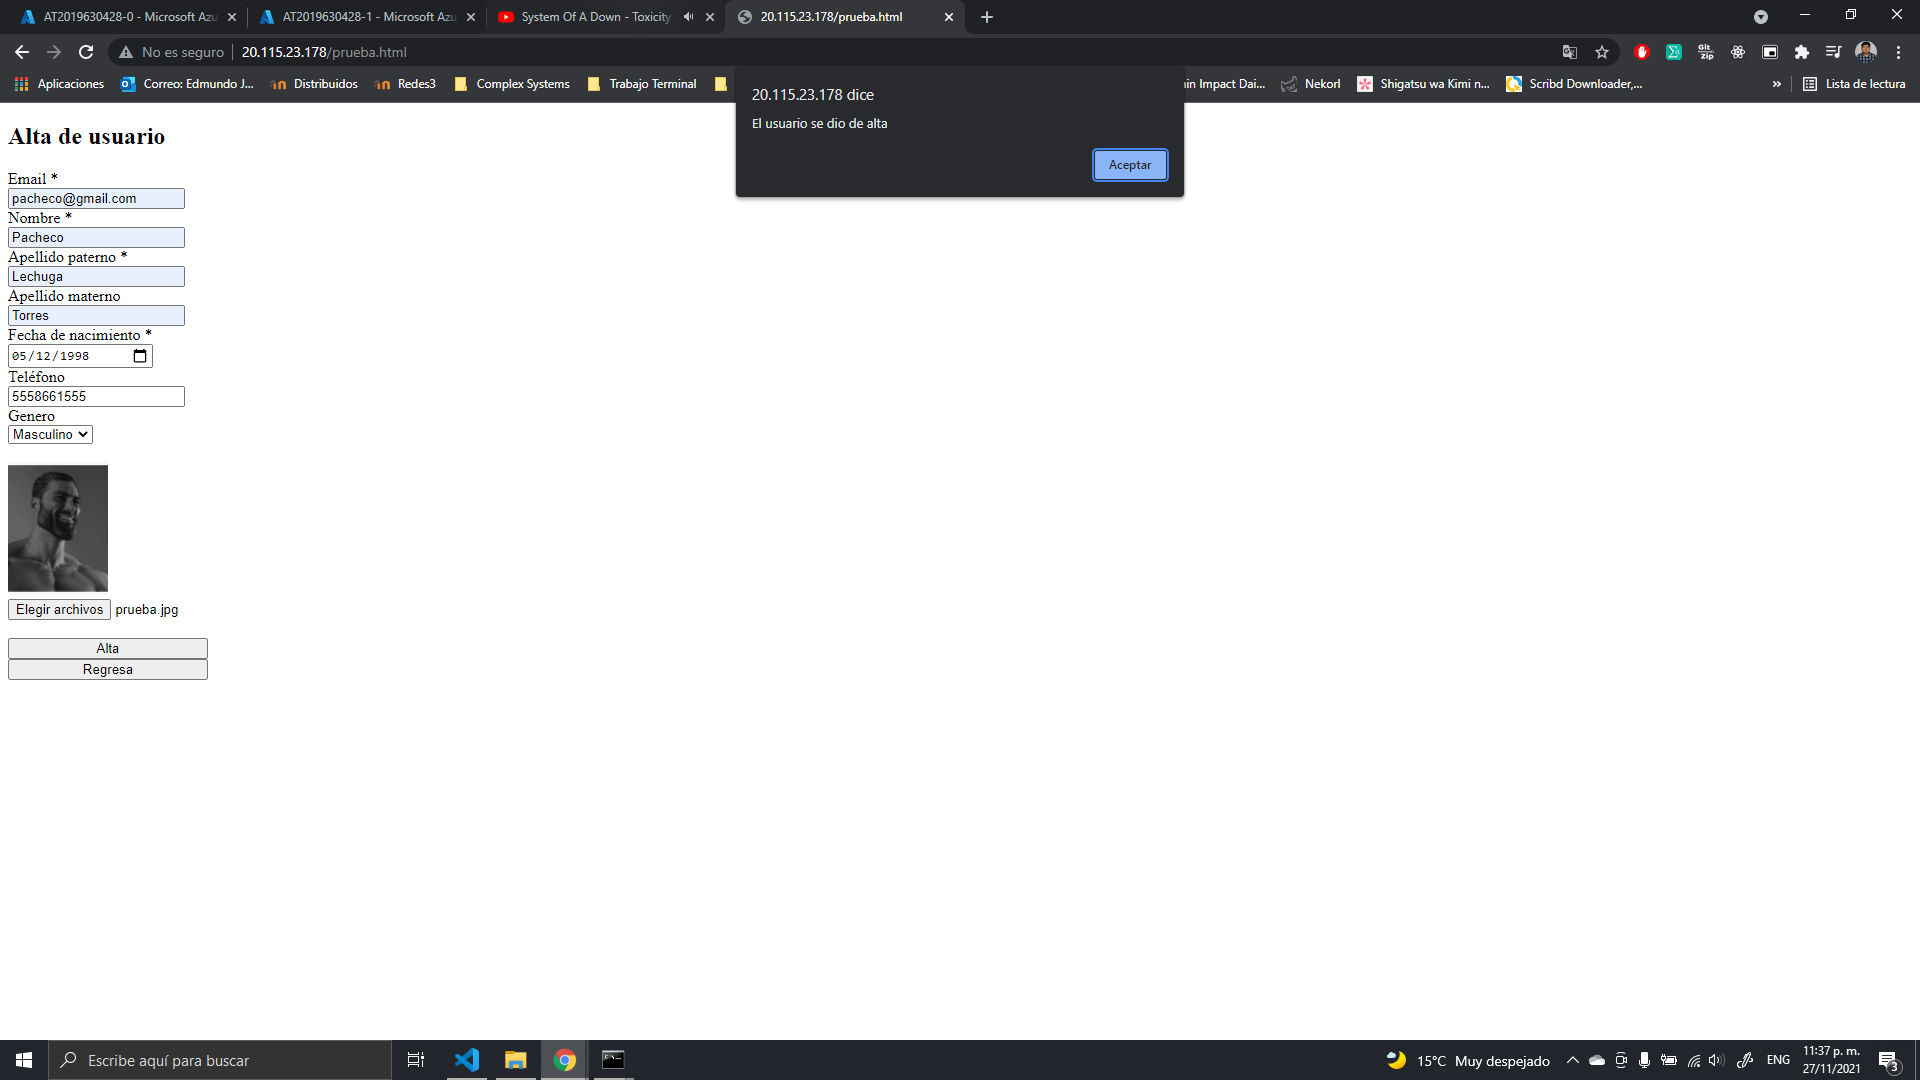
\includegraphics[scale=0.34]{resources/p9.2.1.png}
			\caption{Mensaje de que el alta de usuario fue realizada de manera exitosa.}\label{fig:picture}
		\end{figure}	
		\subsection{Mostrar los registros insertados en la base de datos en la maquina virtual principal y la réplica (no desplegar el contenido del campo foto).}
		En esta parte veremos el contenido de la base de datos con el usuario registrado tanto en el sistema principal como en al replica, en esto en las siguientes dos figuras.
		\begin{figure}[H]
			\centering
			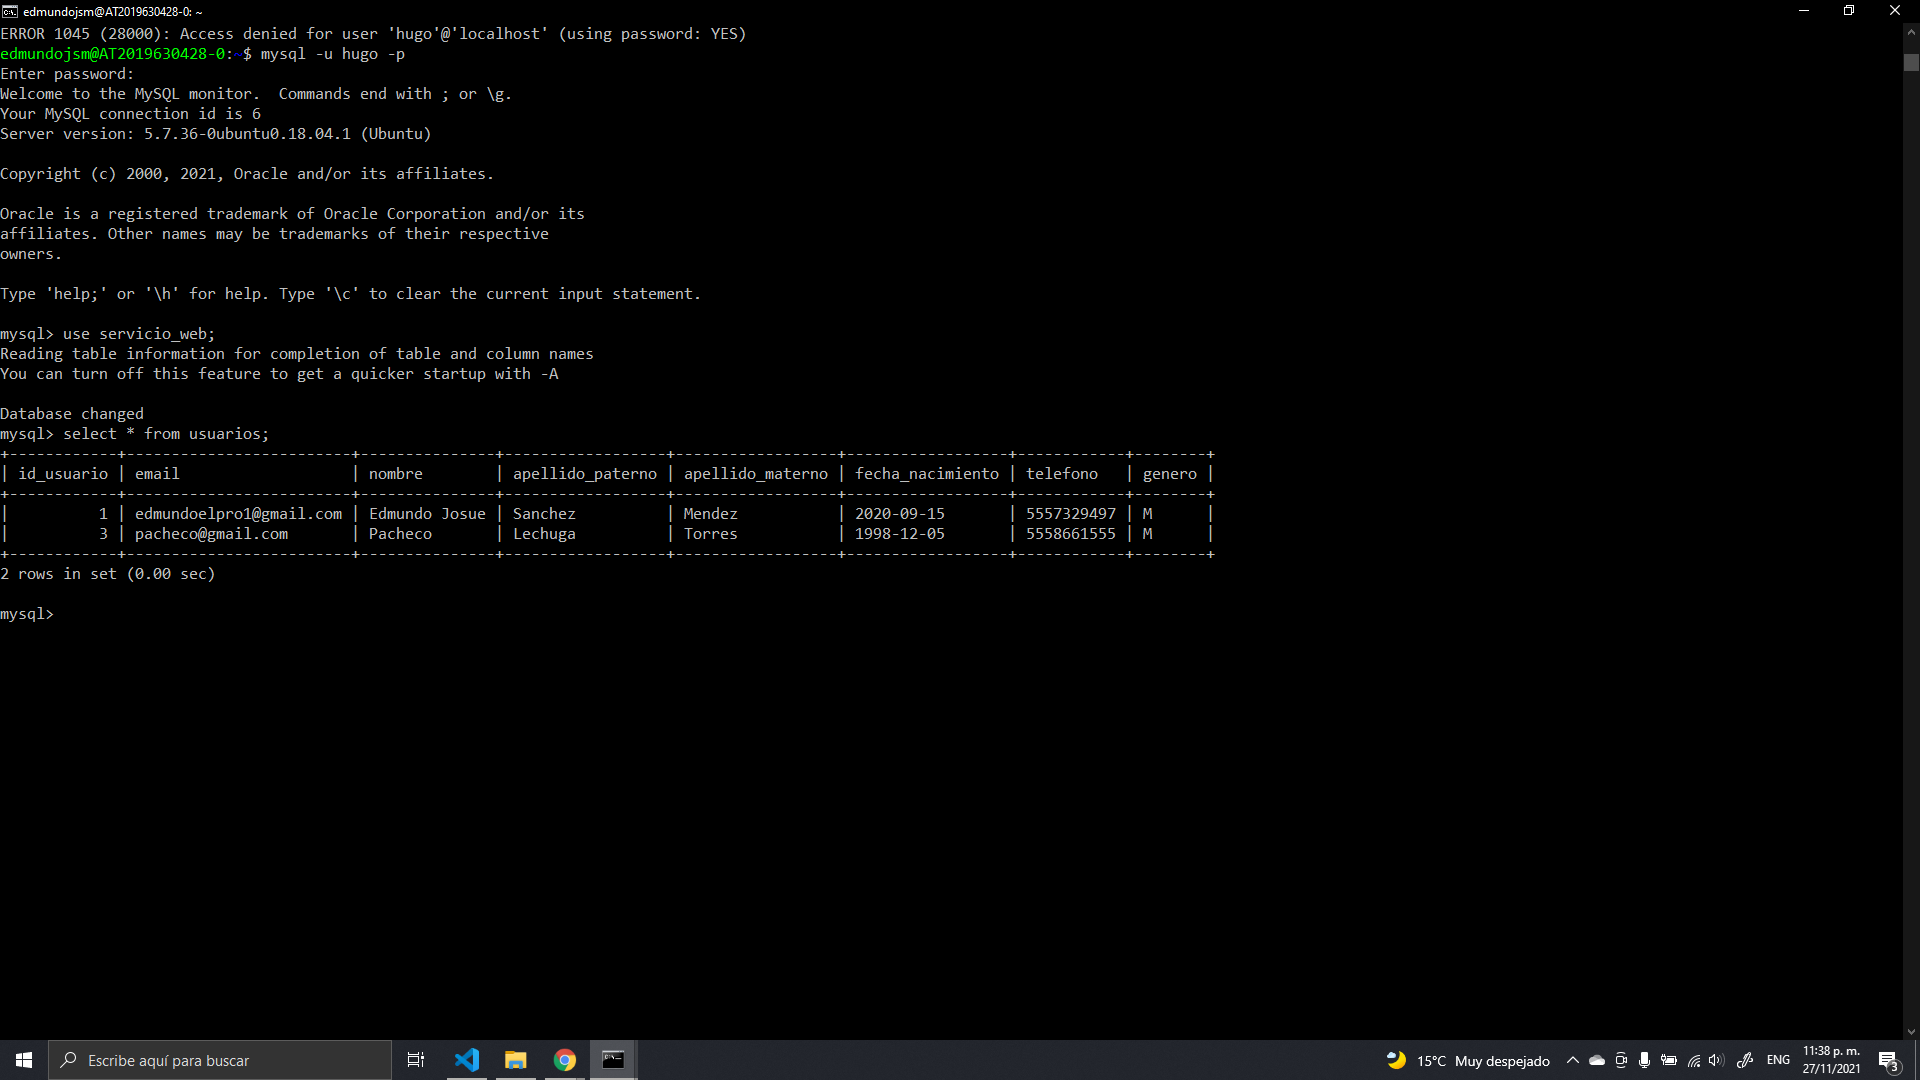
\includegraphics[scale=0.34]{resources/p9.3principal.png}
			\caption{Contenido de la tabla usuario en sistema principal.}\label{fig:picture}
		\end{figure}	
		\begin{figure}[H]
			\centering
			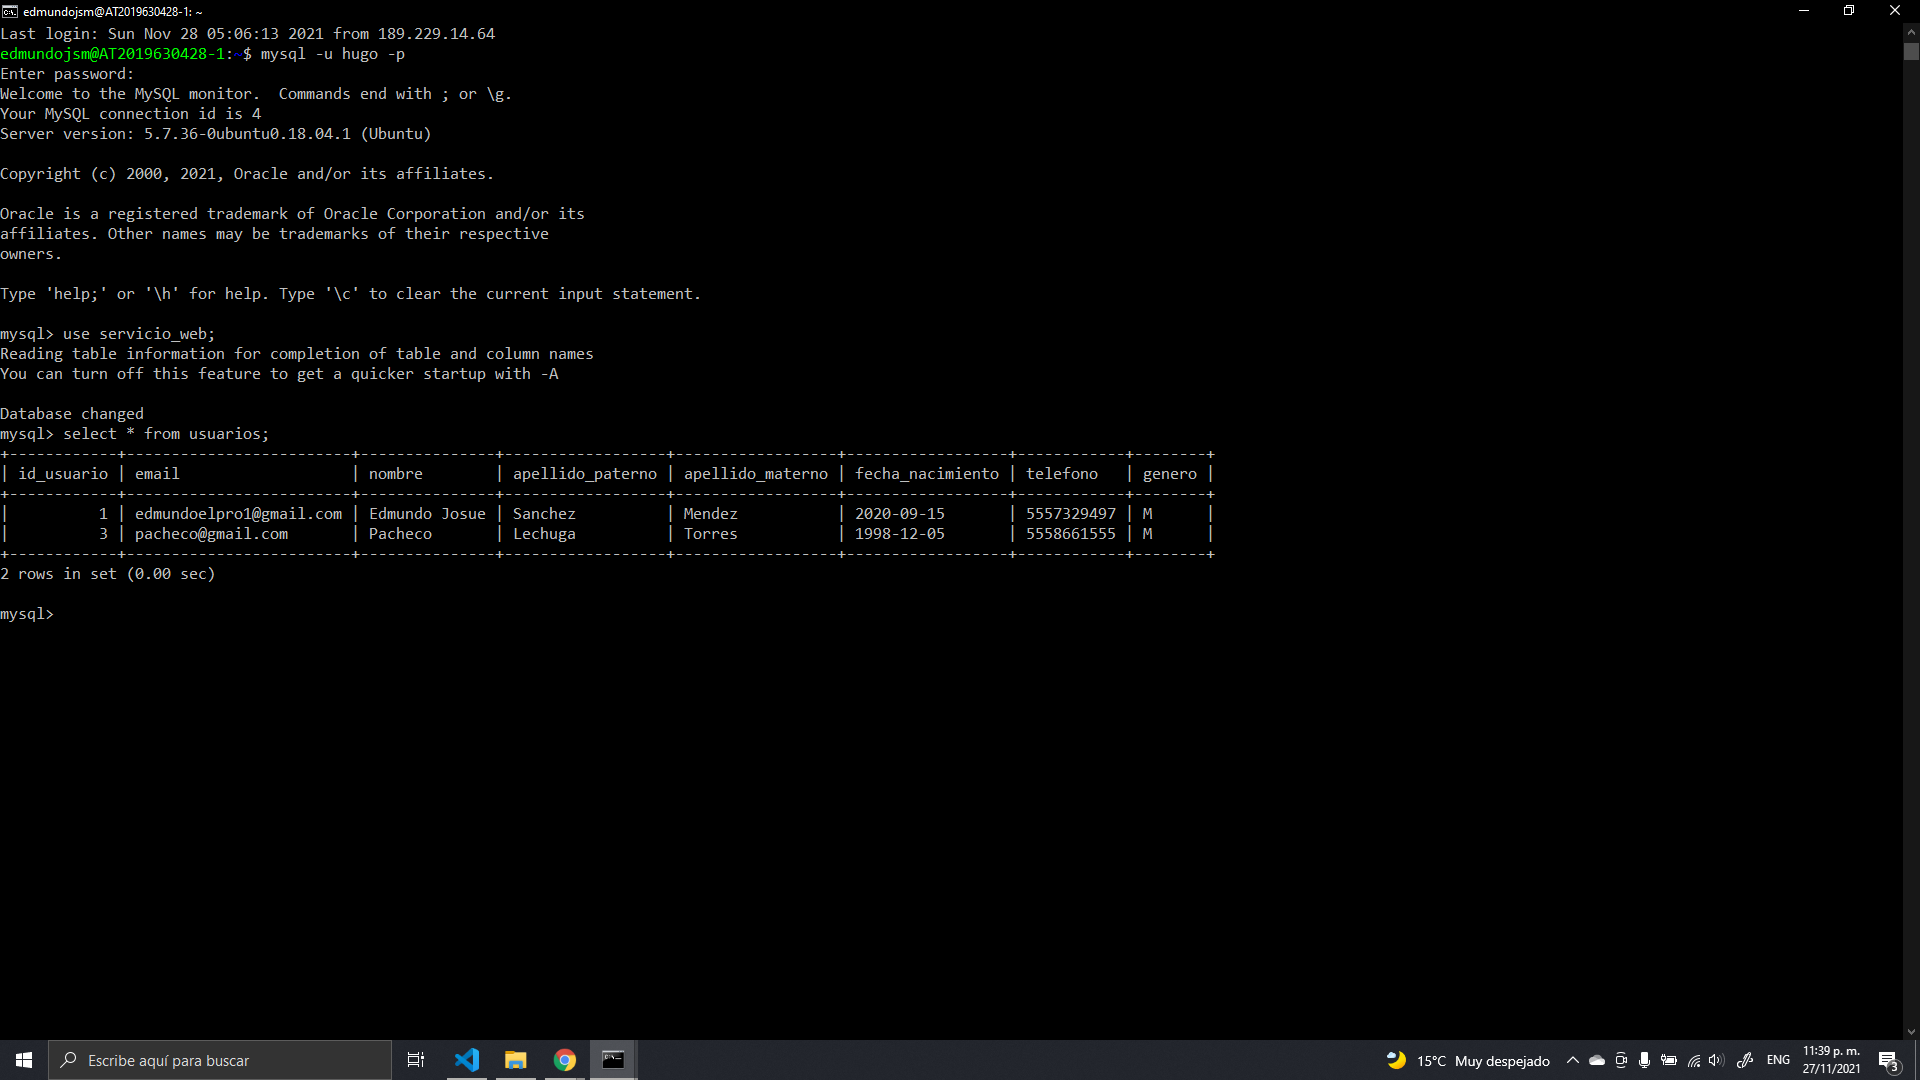
\includegraphics[scale=0.34]{resources/p9.3copia.png}
			\caption{Contenido de la tabla usuario en sistema copia.}\label{fig:picture}
		\end{figure}	
		\subsection{Dar clic en el botón ``Consulta usuario'' para consultar el usuario dado de alta en el paso 5.  Capturar el email y dar clic en el botón ``Consulta''.}
		Consulta de usuario por medio del email al consultar vemos como nos muestra la información que se registro en las pruebas anteriores.
		\begin{figure}[H]
			\centering
			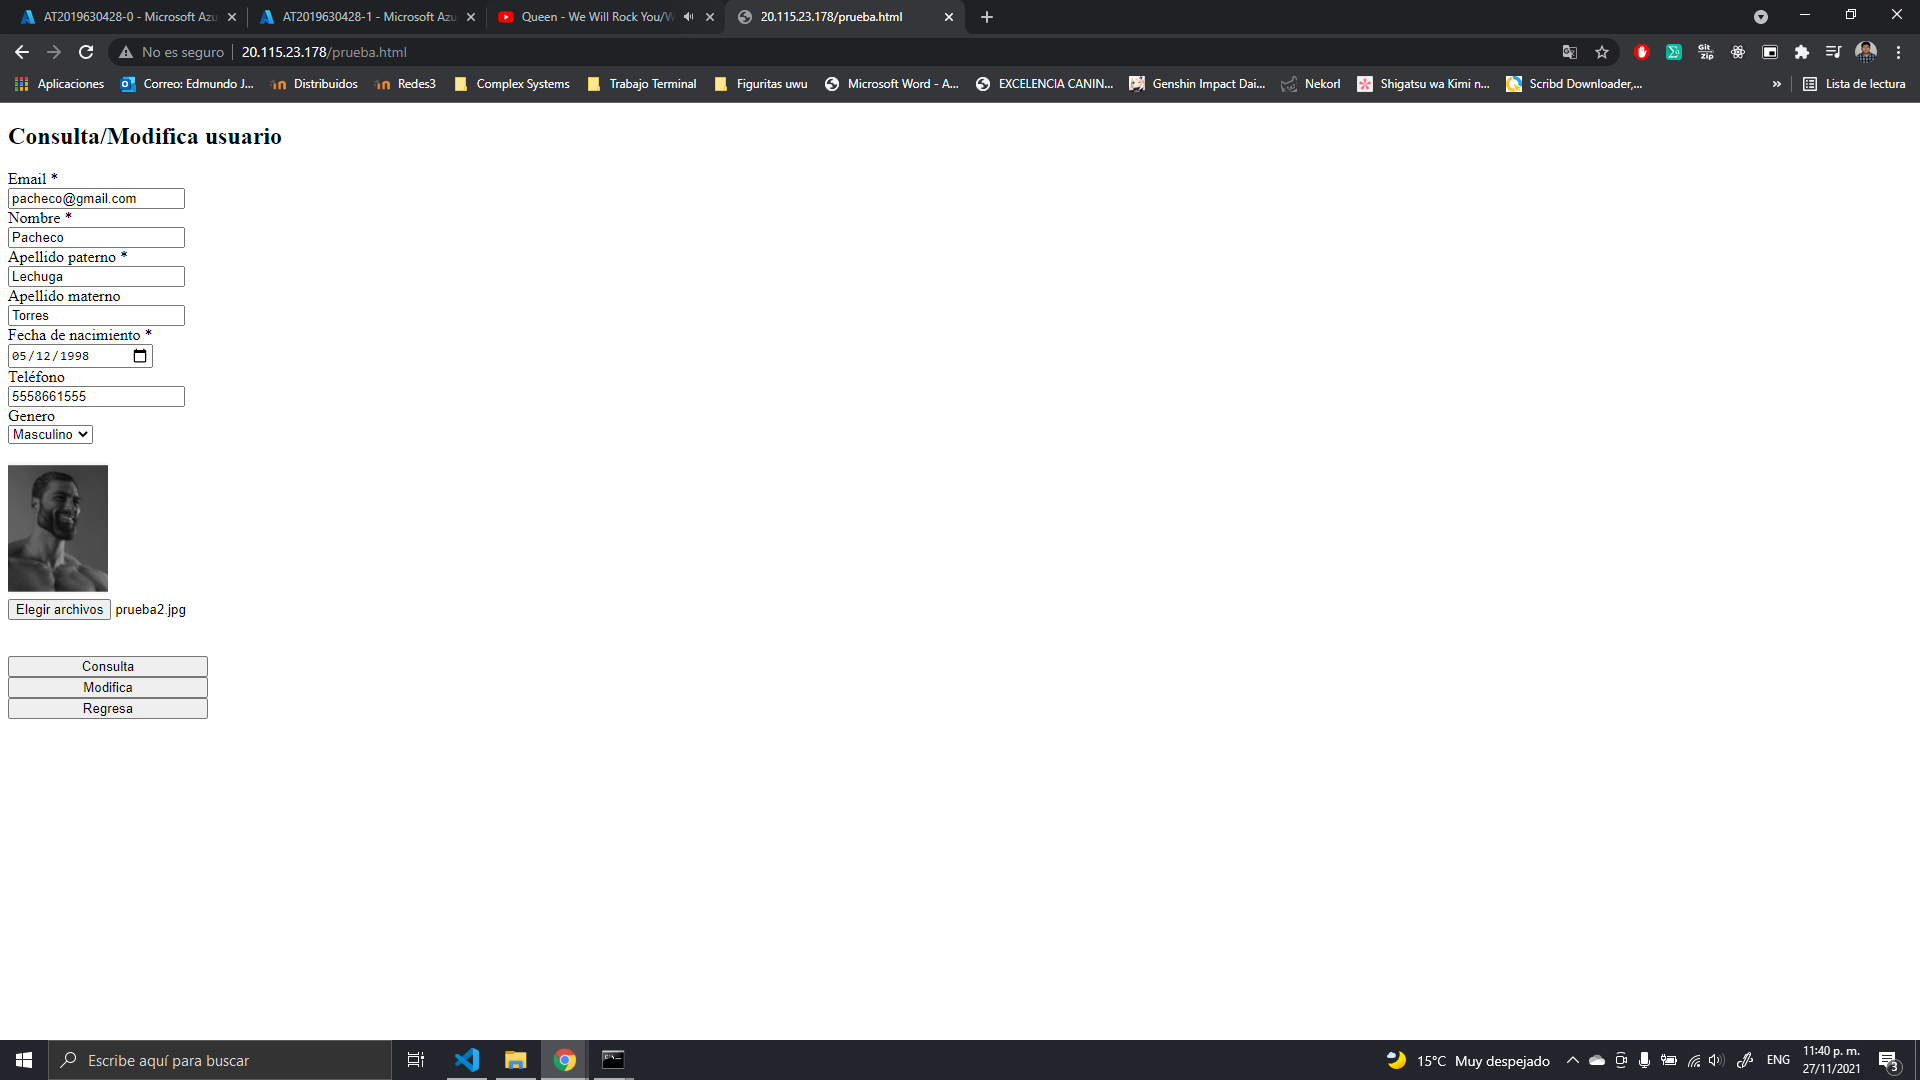
\includegraphics[scale=0.34]{resources/p9.4.png}
			\caption{Consulta del usuario dado de alta en el punto anterior.}\label{fig:picture}
		\end{figure}
		\subsection{Modificar algún dato del usuario y dar clic en el botón ``Modifica''.}
		Modificación de nombre, apellido materno y de foto en el usuario de prueba que es lo que podemos ver en la figura 29 y en la figura 30 vemos el mensaje de que el usuario se modifico de manera exitosa
		\begin{figure}[H]
			\centering
			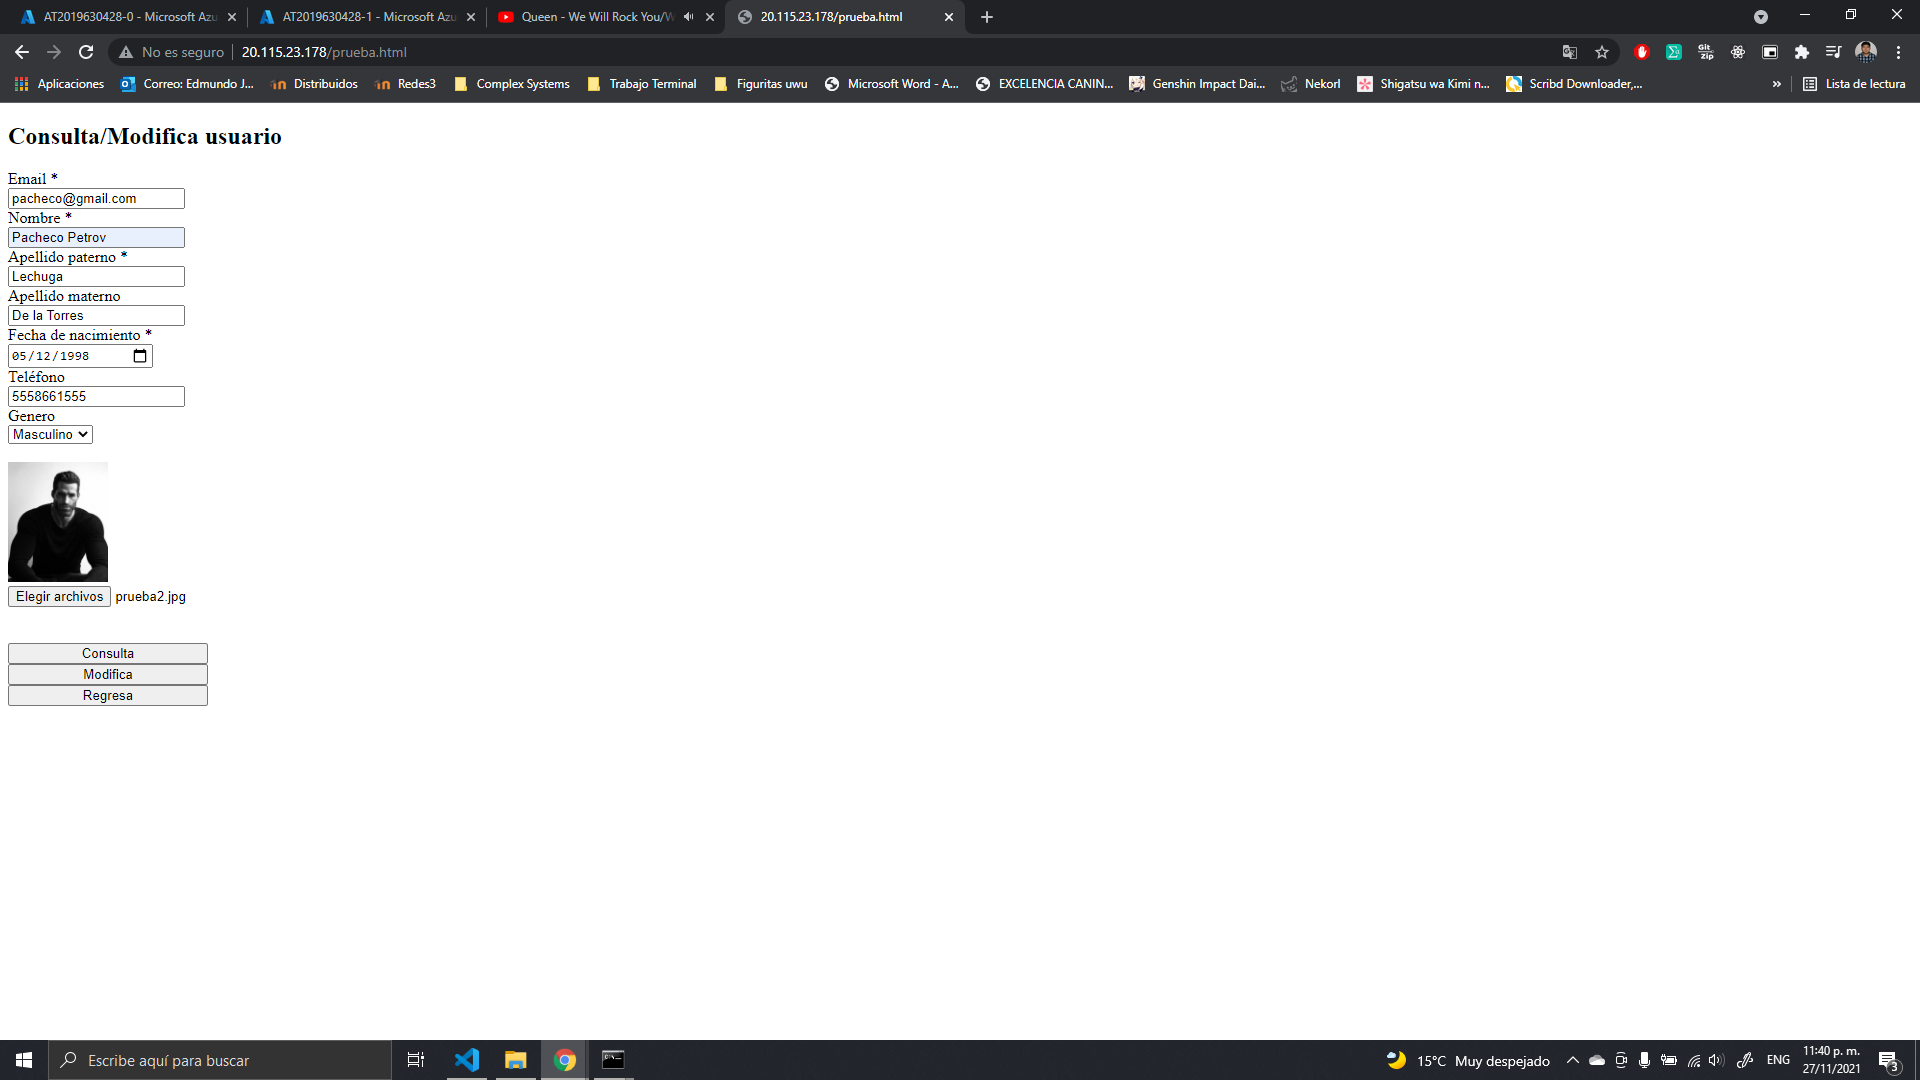
\includegraphics[scale=0.34]{resources/p9.5.png}
			\caption{Modificación del usuario prueba.}\label{fig:picture}
		\end{figure}
		\begin{figure}[H]
			\centering
			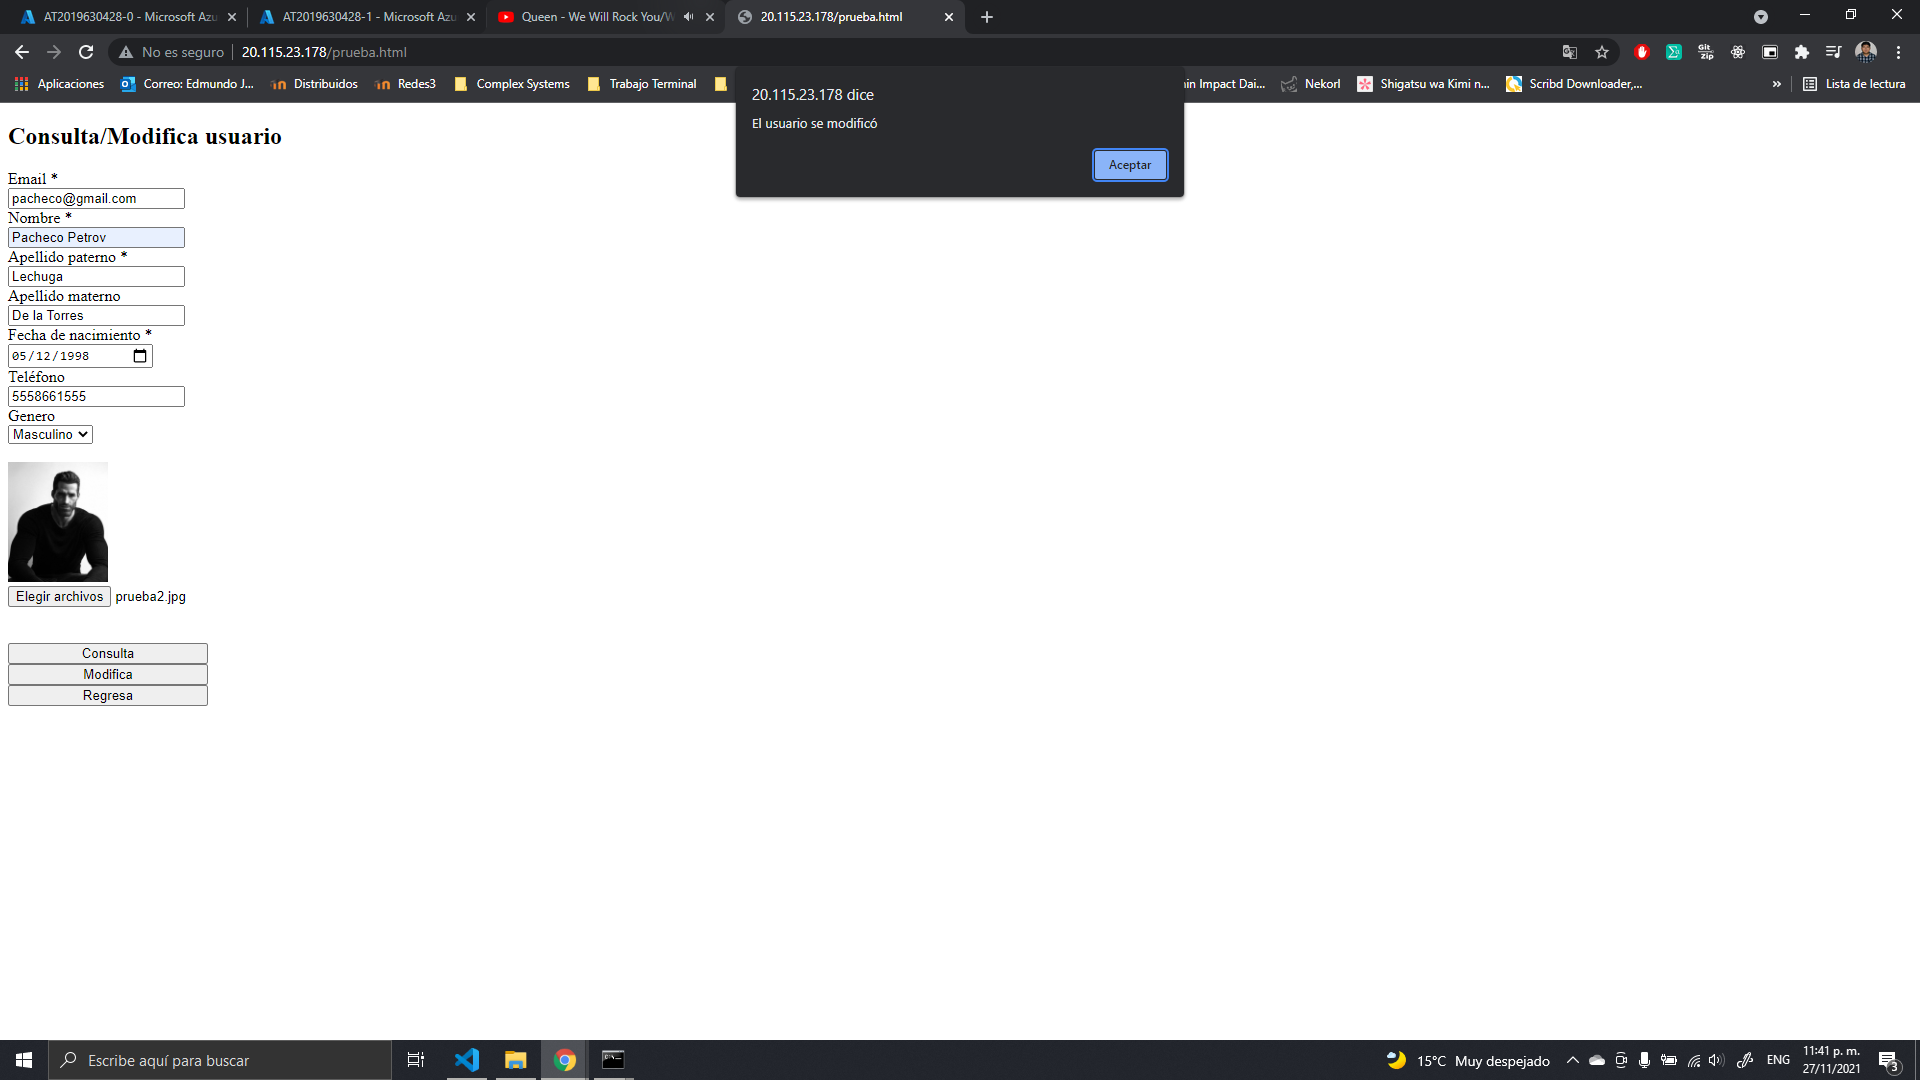
\includegraphics[scale=0.34]{resources/p9.5.1.png}
			\caption{Modificación del usuario realizado de manera correcta.}\label{fig:picture}
		\end{figure}
		\subsection{Mostrar los registros modificados en la base de datos en la maquina virtual principal y la réplica.}
		En esta parte veremos el contenido de la base de datos con el usuario modificado tanto en el sistema principal como en al replica, en esto en las siguientes dos figuras.
		\begin{figure}[H]
			\centering
			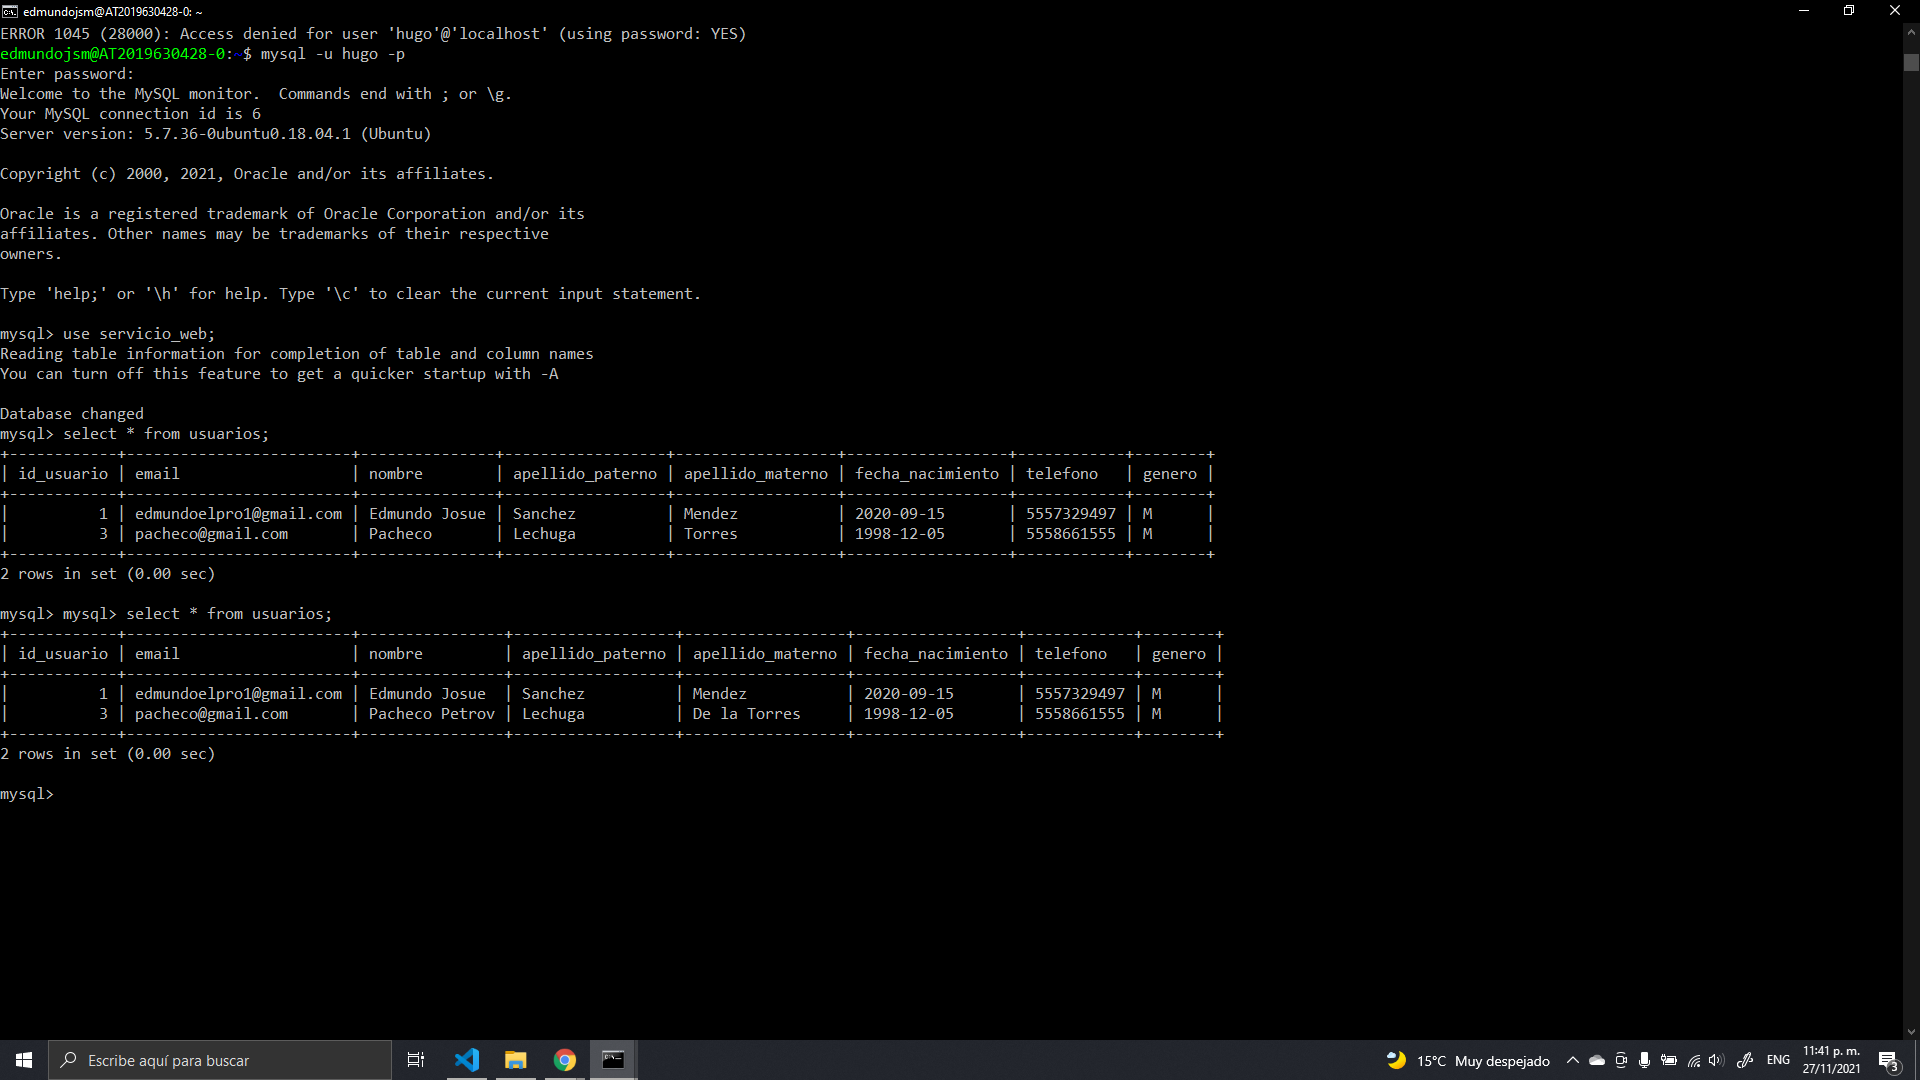
\includegraphics[scale=0.34]{resources/p9.6principal.png}
			\caption{Contenido de la tabla usuario en sistema principal.}\label{fig:picture}
		\end{figure}	
		\begin{figure}[H]
			\centering
			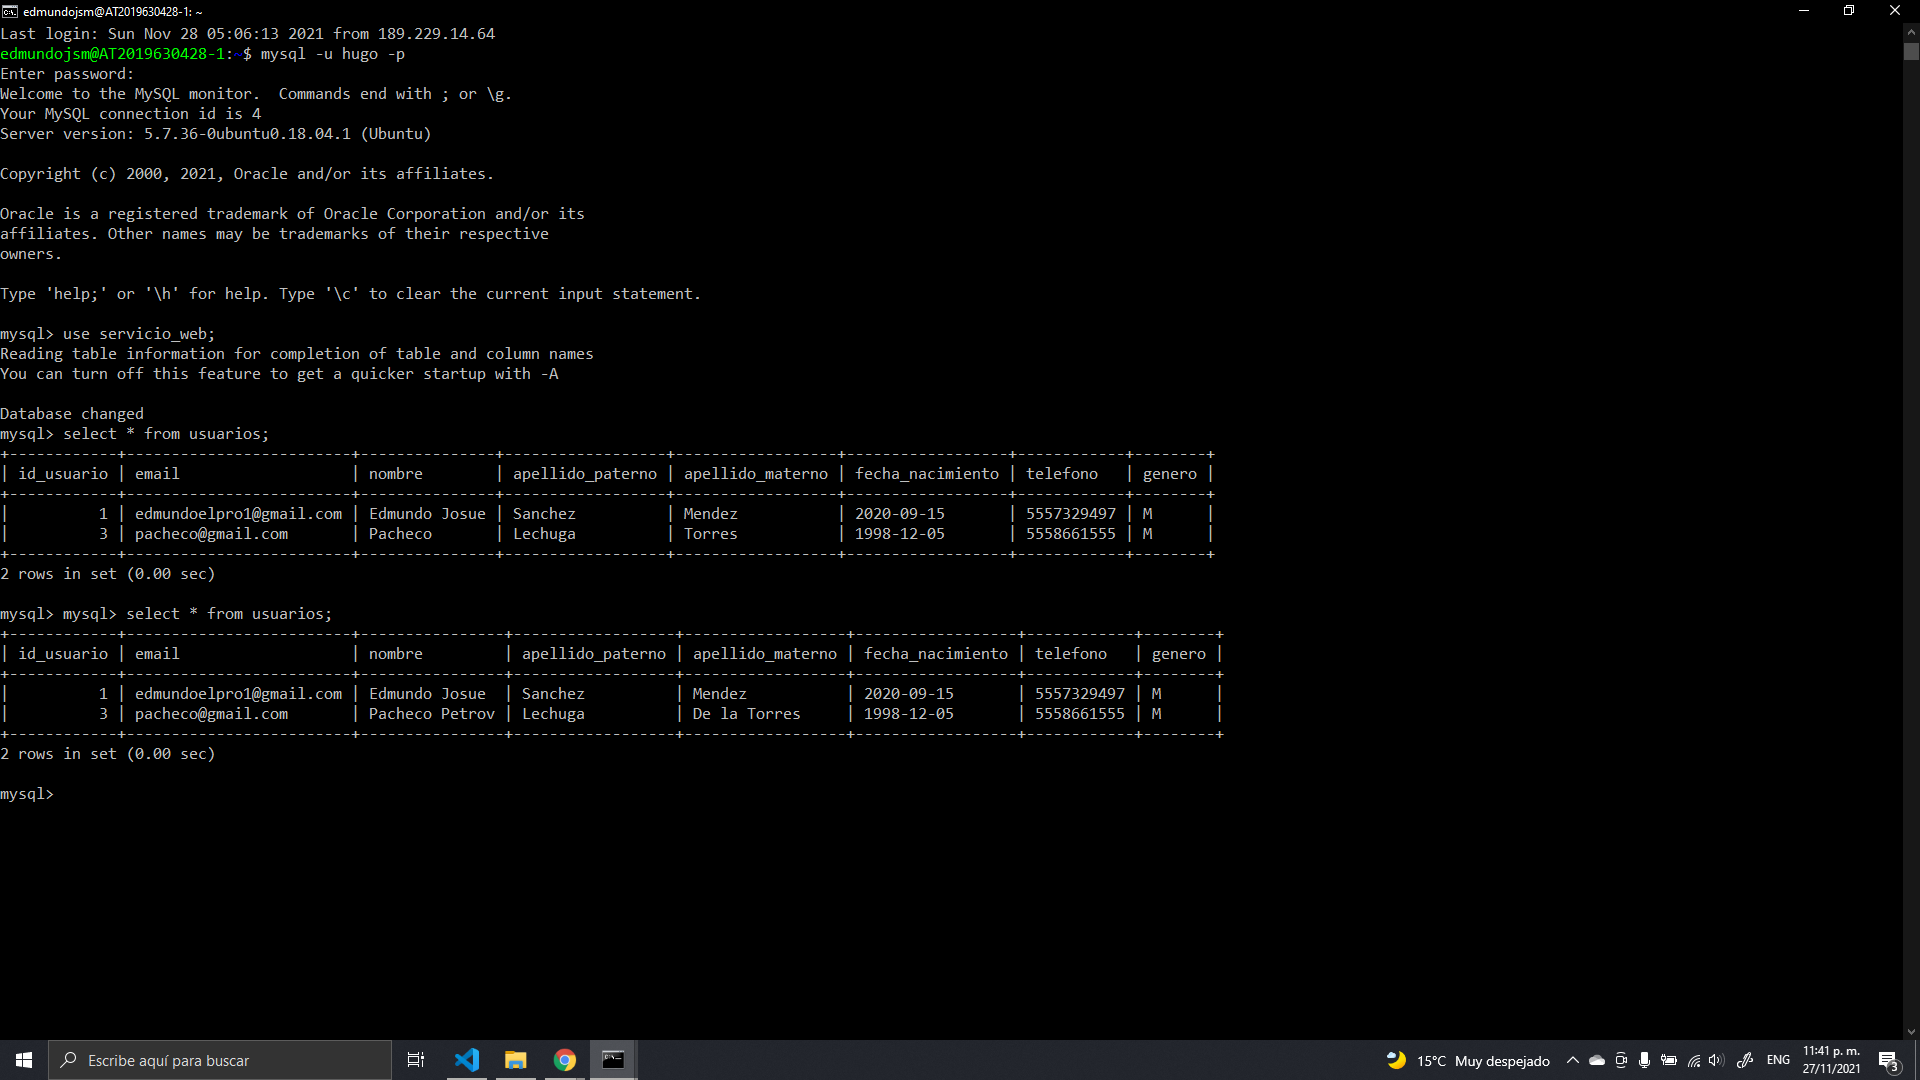
\includegraphics[scale=0.34]{resources/p9.6copia.png}
			\caption{Contenido de la tabla usuario en sistema copia.}\label{fig:picture}
		\end{figure}
		\subsection{Consultar el usuario modificado, para verificar que la modificación se realizó.}
		Consulta de usuario por medio del email al consultar vemos como nos muestra la información actualizado del usuario de las pruebas anteriores.
		\begin{figure}[H]
			\centering
			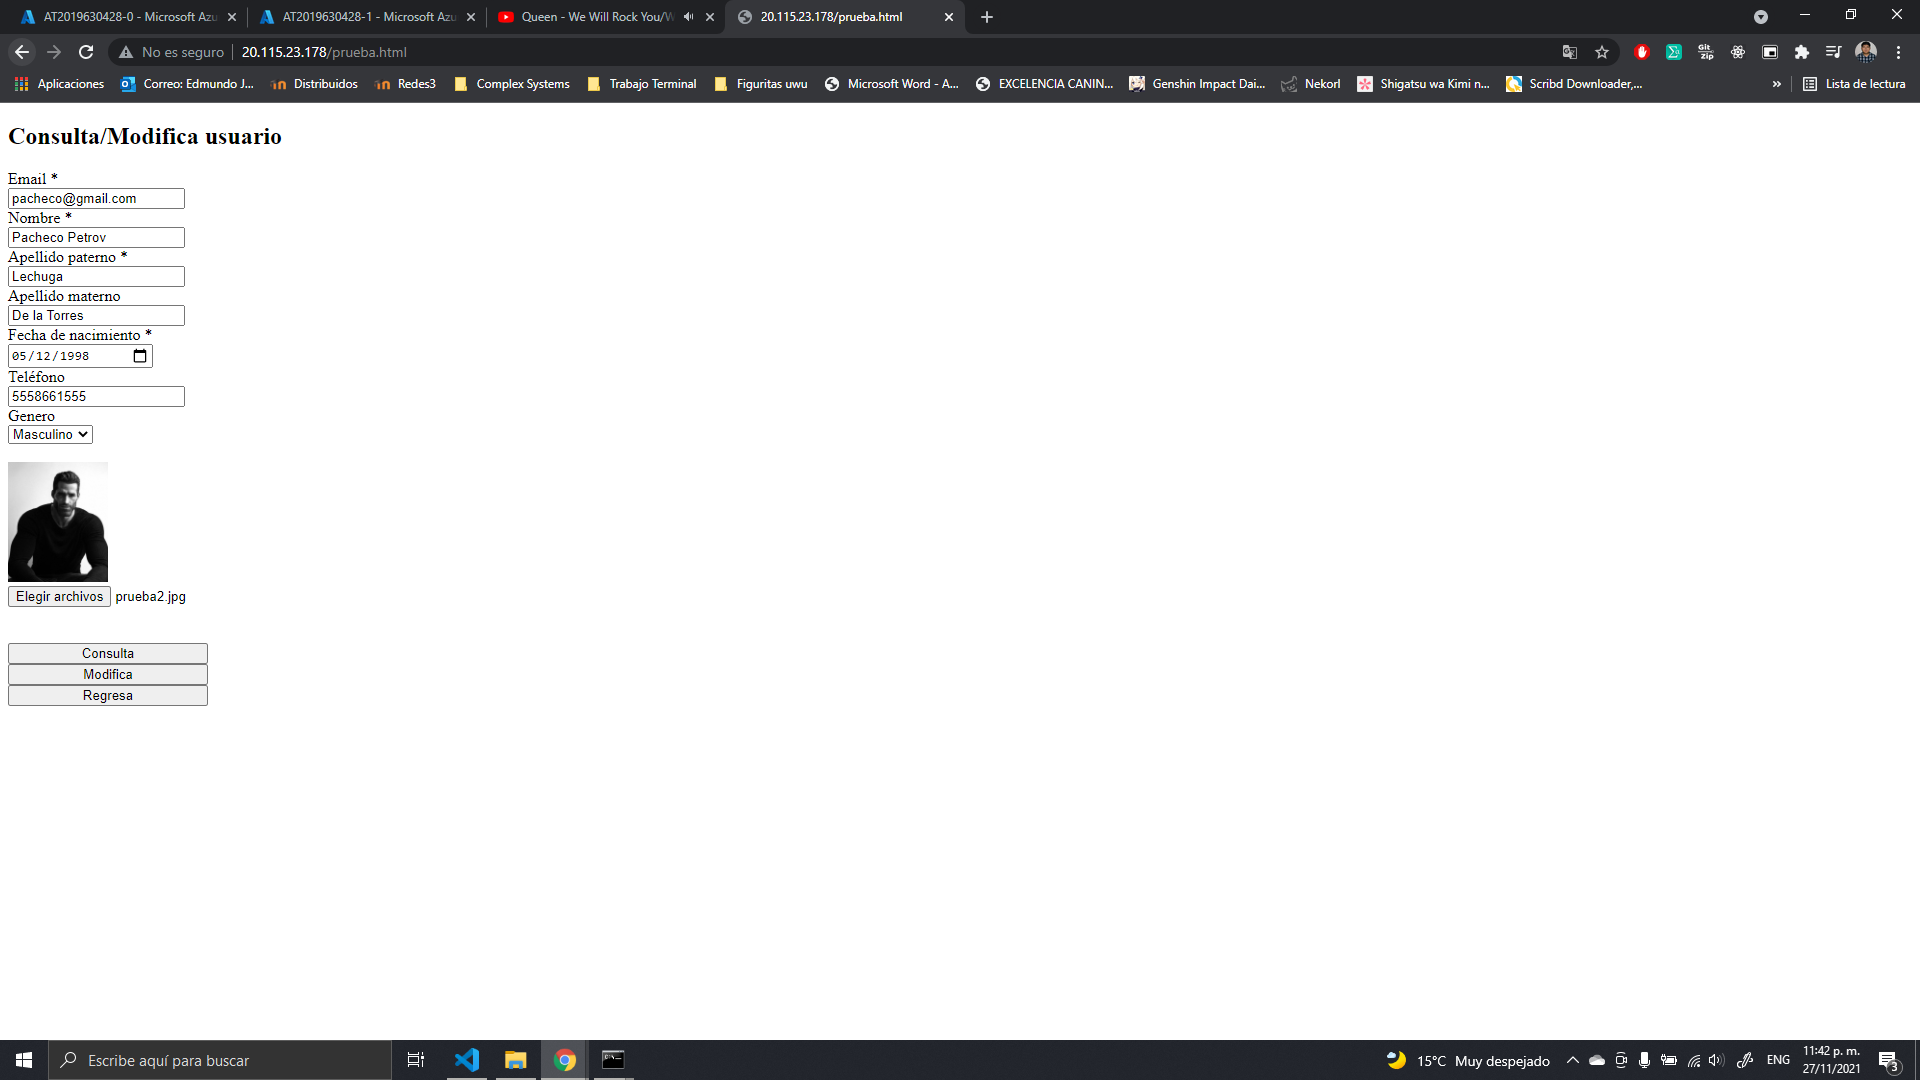
\includegraphics[scale=0.34]{resources/p9.7.png}
			\caption{Consulta del usuario modificado en puntos anteriores.}\label{fig:picture}
		\end{figure}
		\subsection{Dar clic en el botón ``Borra usuario'' para borrar el usuario.}
		En esta prueba eliminaremos al usuario creado para las pruebas, en la figura 33 podemos ver que ingresamos el correo registrado en la base de datos y en la figura 34 vemos el mensaje de que el usuario se borro de manera exitosa.
		\begin{figure}[H]
			\centering
			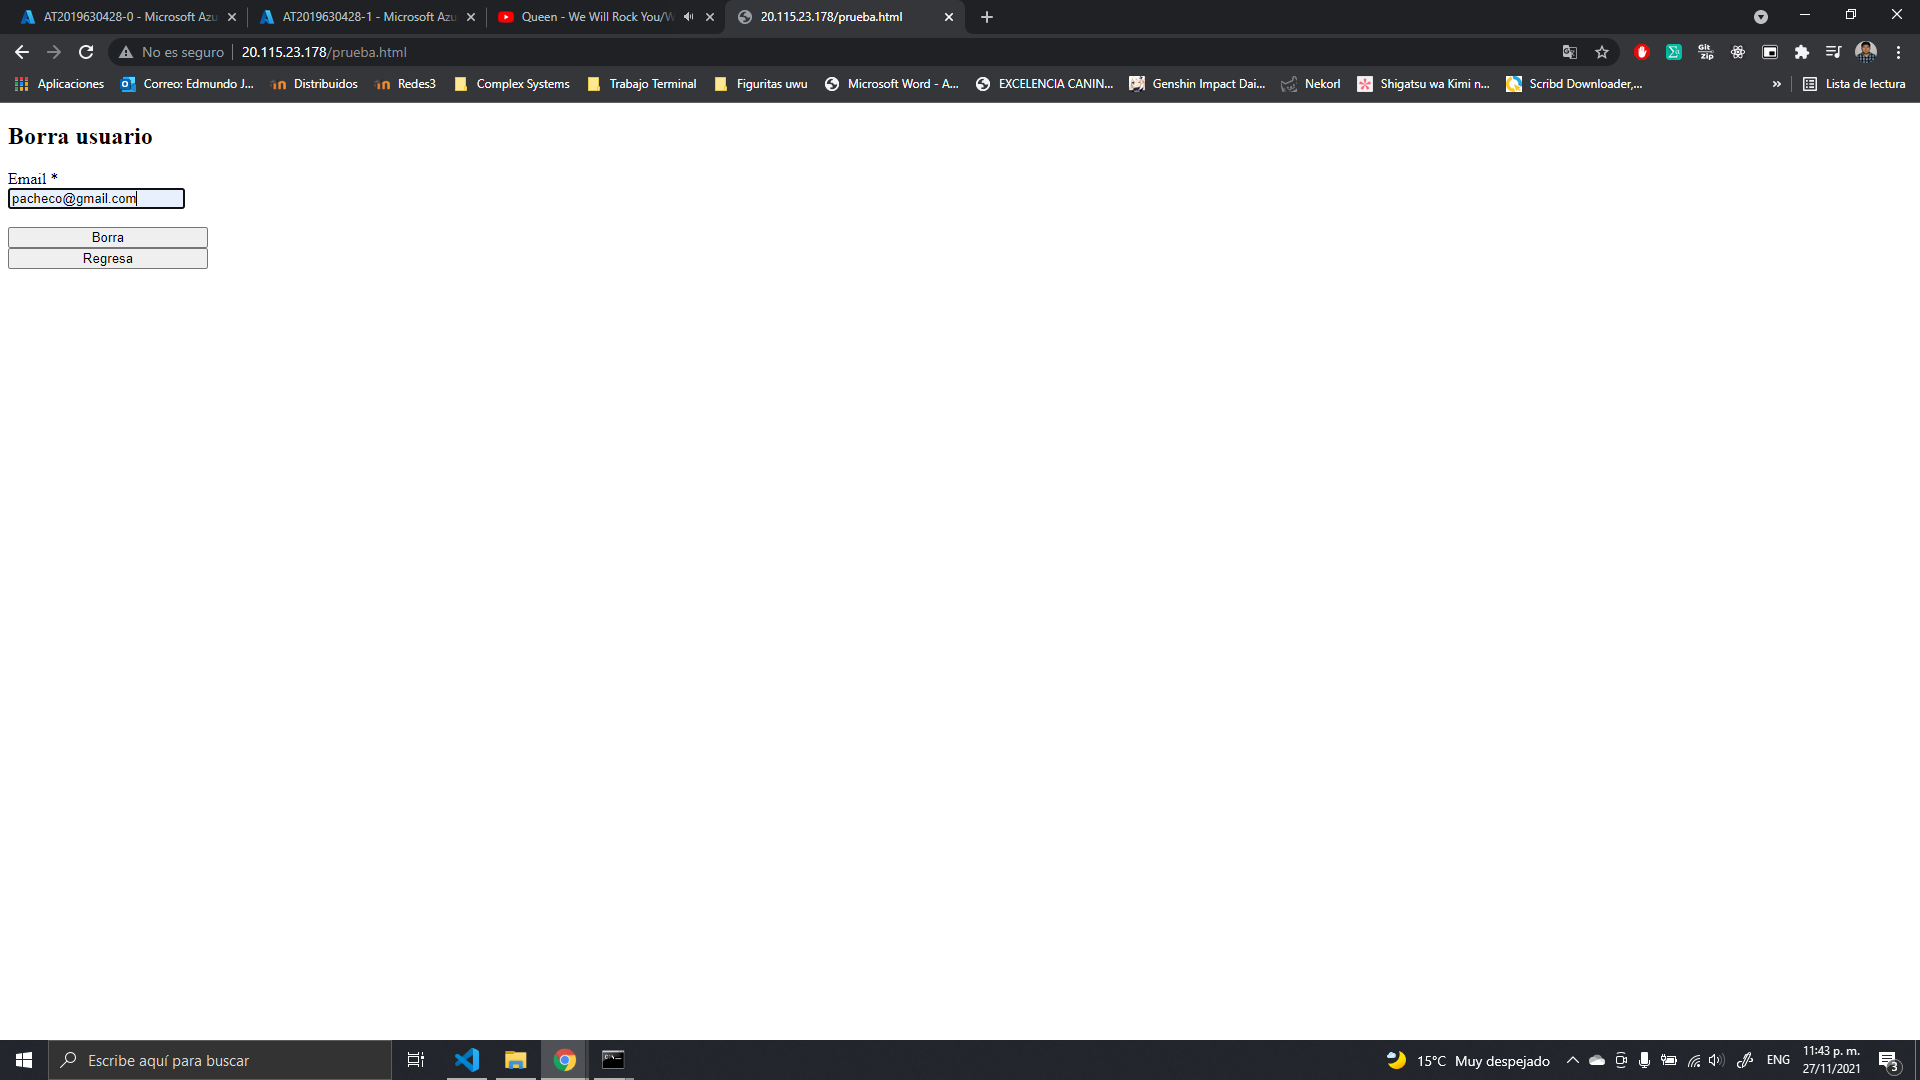
\includegraphics[scale=0.34]{resources/p9.8.png}
			\caption{Ingreso del correo para poder borrarlo.}\label{fig:picture}
		\end{figure}
		\begin{figure}[H]
			\centering
			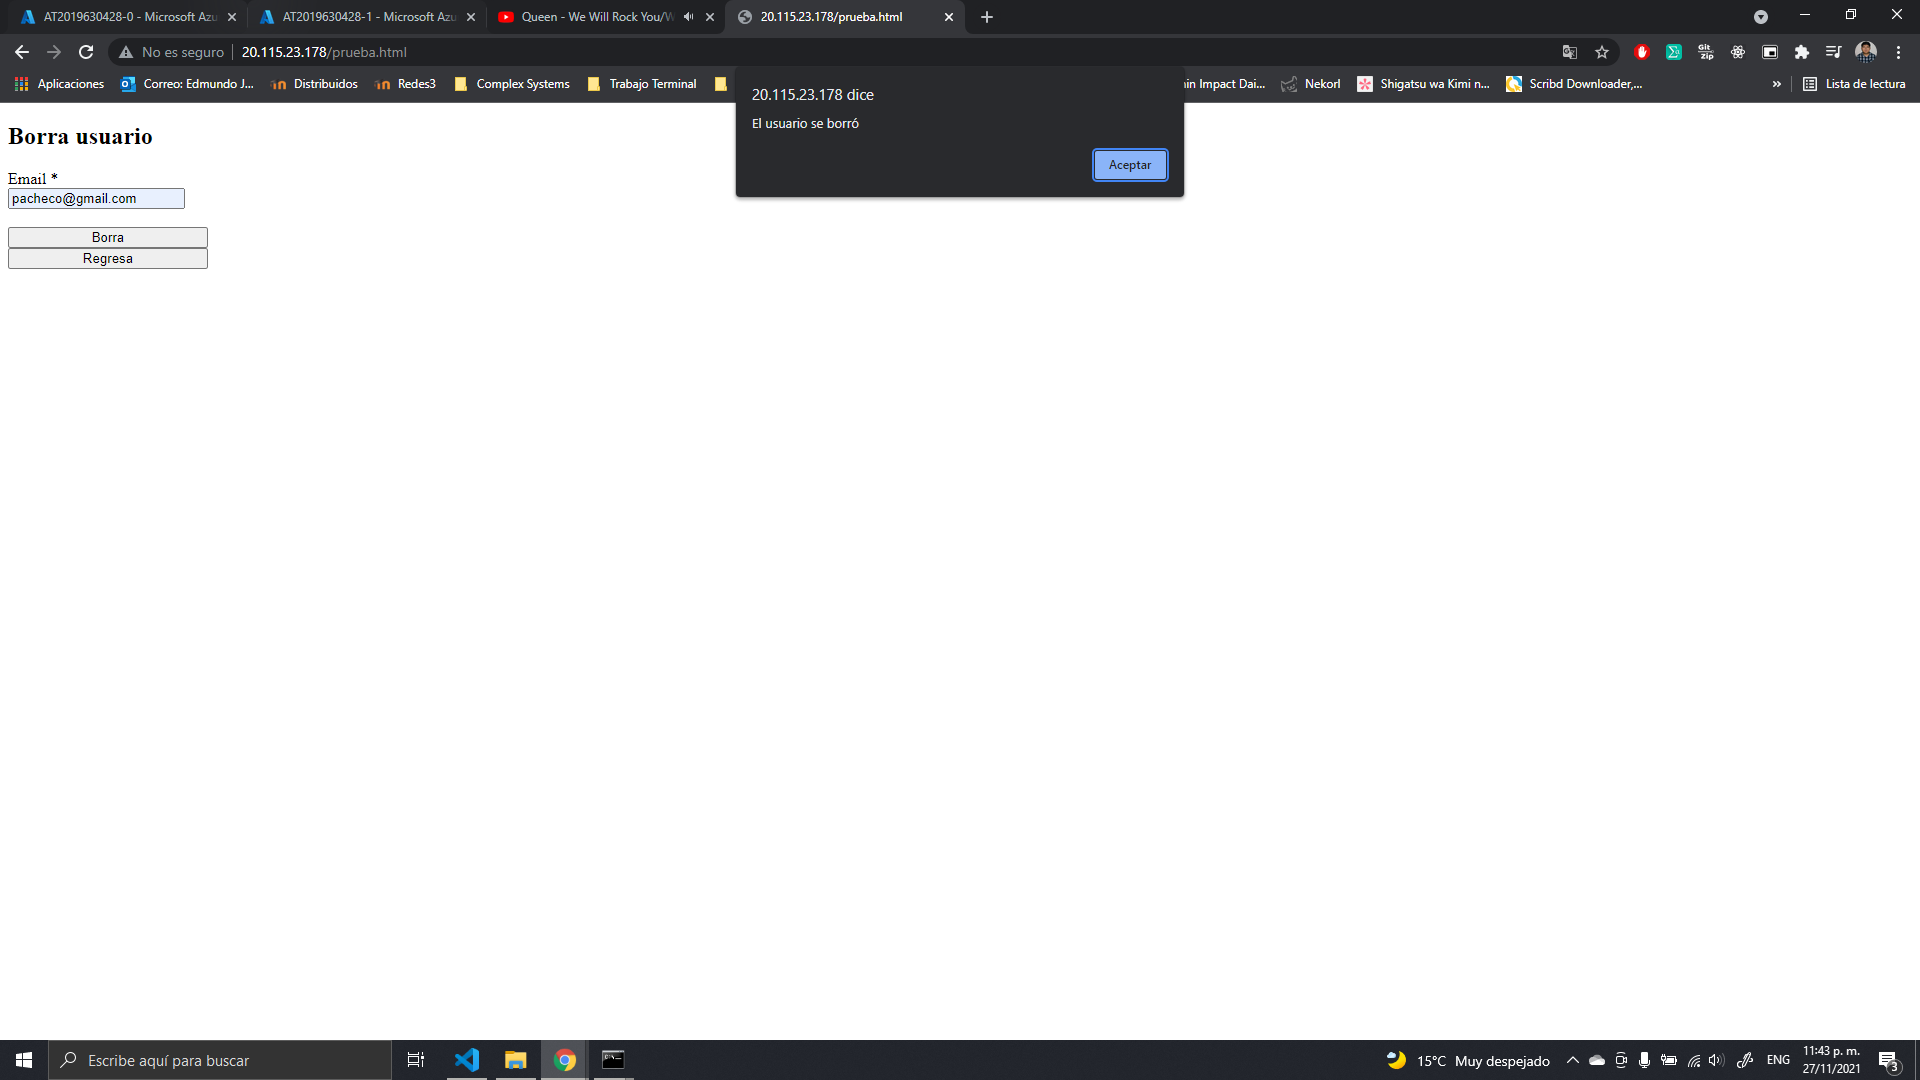
\includegraphics[scale=0.34]{resources/p9.8.1.png}
			\caption{Eliminación del usuario realizado de manera correcta.}\label{fig:picture}
		\end{figure}
		\subsection{Mostrar los registros insertados en la base de datos en la maquina virtual principal y la réplica.}
		En esta parte veremos el contenido de la base de datos con el usuario eliminado tanto en el sistema principal como en al replica, en esto en las siguientes dos figuras.
		\begin{figure}[H]
			\centering
			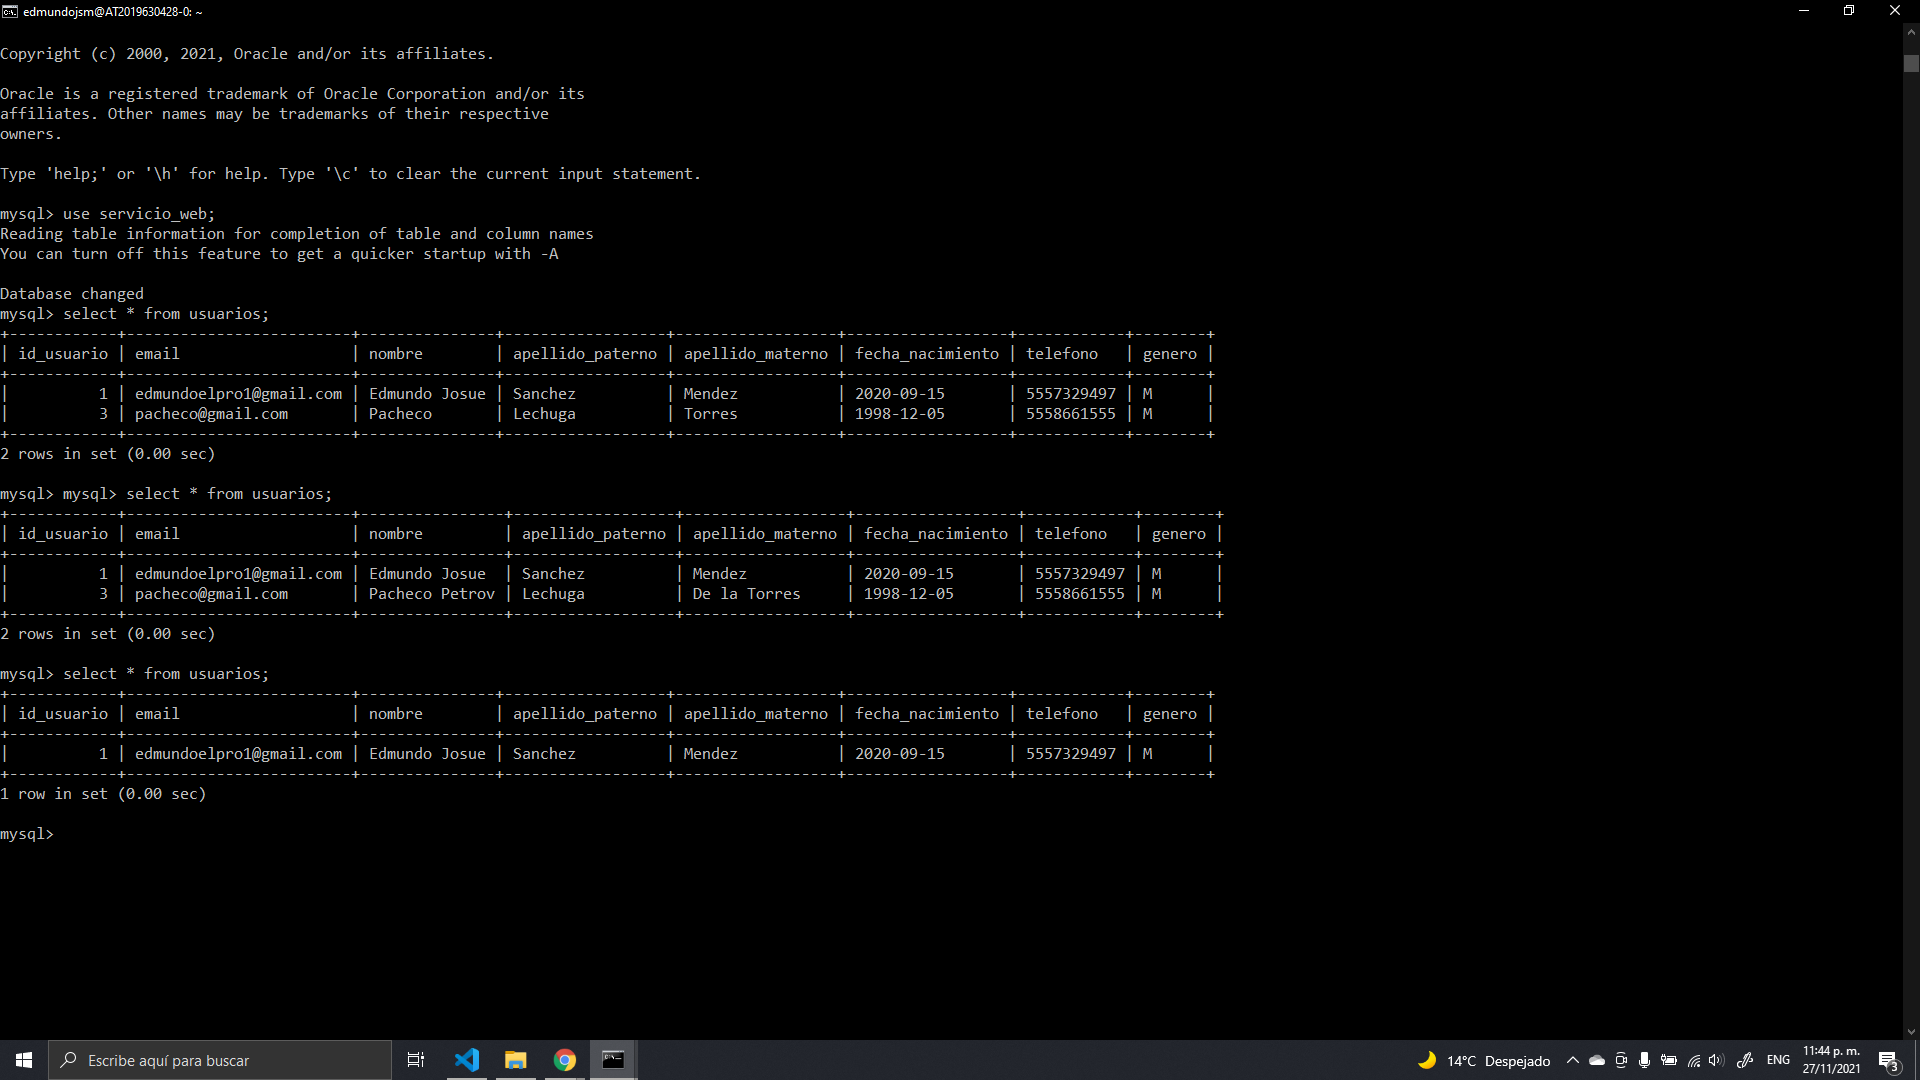
\includegraphics[scale=0.34]{resources/p9.9principal.png}
			\caption{Contenido de la tabla usuario en sistema principal.}\label{fig:picture}
		\end{figure}	
		\begin{figure}[H]
			\centering
			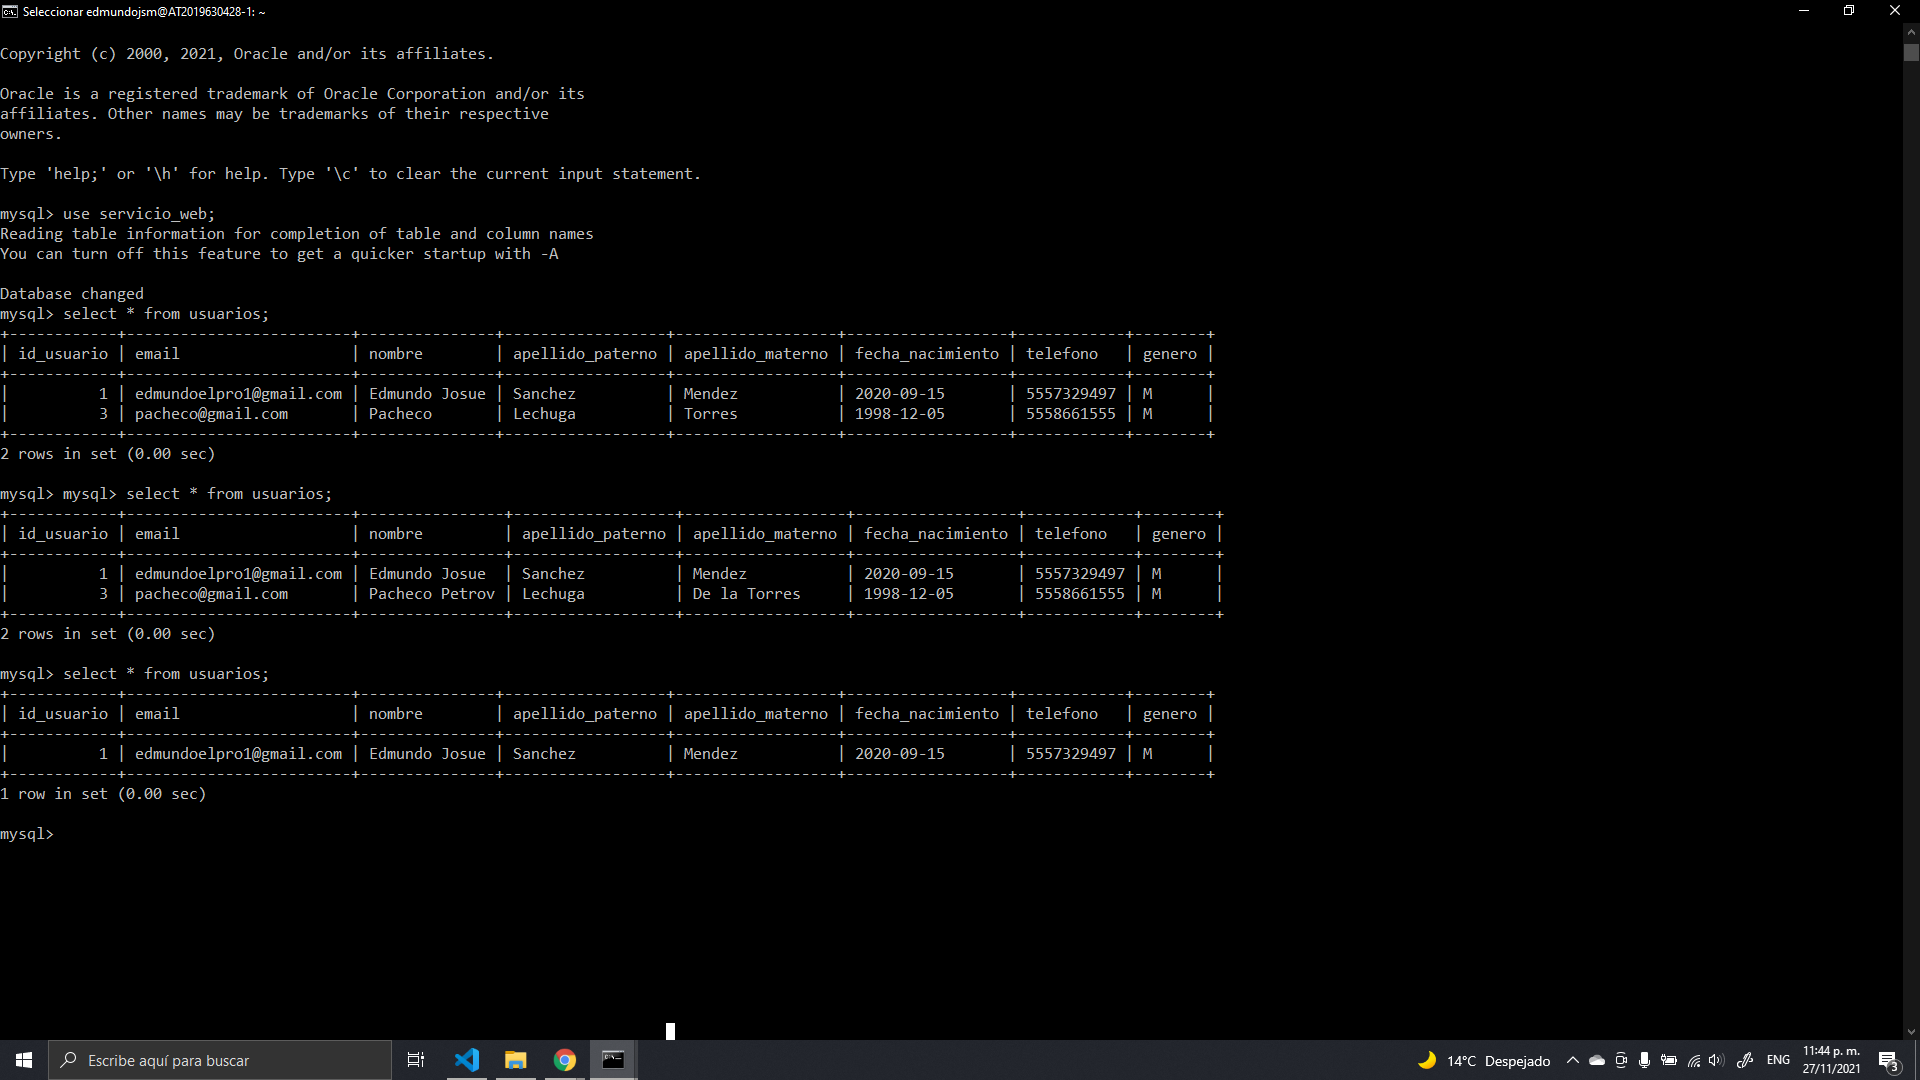
\includegraphics[scale=0.34]{resources/p9.9copia.png}
			\caption{Contenido de la tabla usuario en sistema copia.}\label{fig:picture}
		\end{figure}	
		\subsection{Capturar el email del usuario borrado y dar clic en el botón ``Consulta''.}
		Consulta de usuario por medio del email al consultar vemos como no nos muestra la información del usuario de las pruebas anteriores ya que este no existe con un mensaje de alerta de que el usuario no existe.
		\begin{figure}[H]
			\centering
			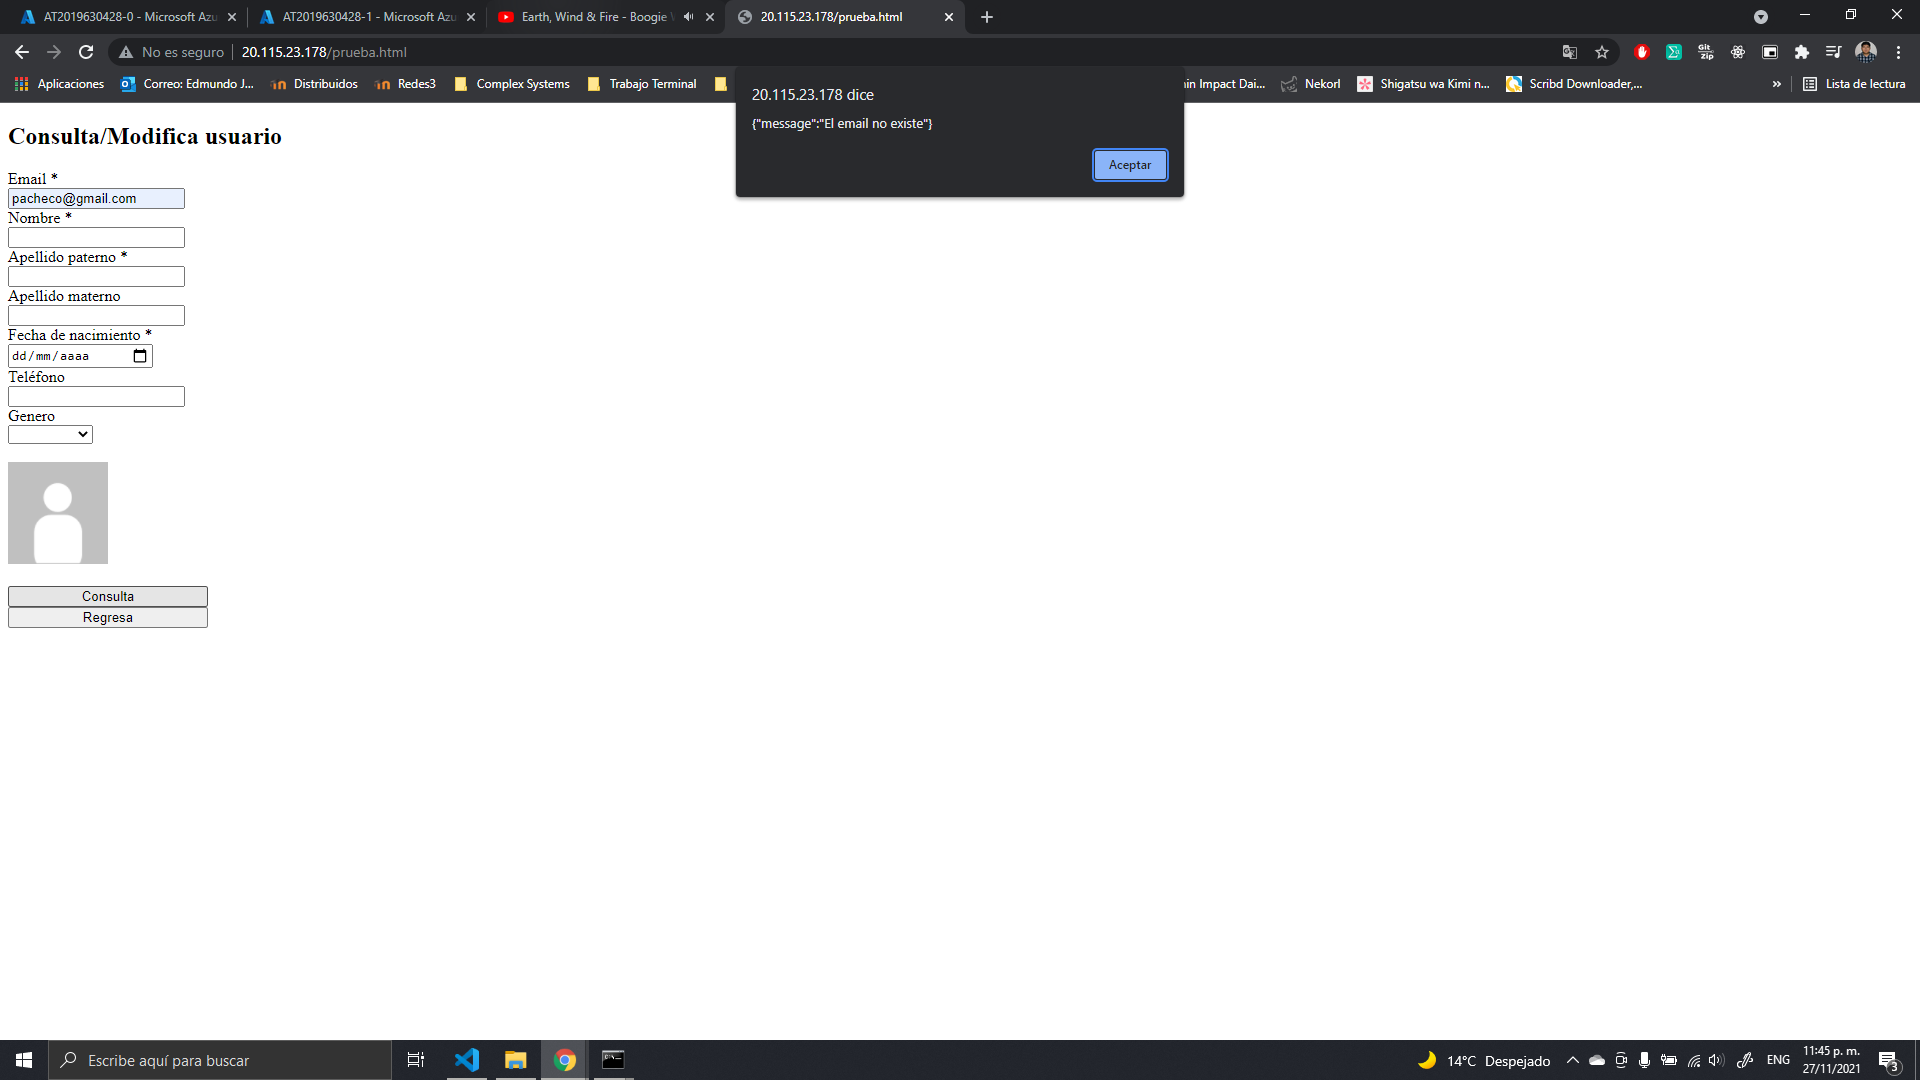
\includegraphics[scale=0.34]{resources/p9.10.png}
			\caption{Consulta del usuario eliminado en puntos anteriores.}\label{fig:picture}
		\end{figure}
		\section{Conclusiones}
	En esta practica pudimos ver como se puede replicar un sistema y como a la vez podemos acceder a sus funcionalidades sin problema alguno, esto nos proporciona ciertos beneficios como lo es la replicación de datos y si en dado caso el sistema principal falla tenemos los datos replicados en nuestro sistema replica y como si creamos una imagen de cualquier maquina virtual los datos que teníamos almacenados seguirán estando en las maquinas que creemos con base en la imagen.
		
\end{document}
